\chapter{一元实值函数的积分}

这一章我们介绍一元实值函数的Riemann 积分理论. 利用积分函数我们严格定义了对数函数、指数函数及幂函数等基本初等函数.

\section{阶梯函数的积分}

\section*{1. 区间的分割}

定义 设 $\left\lbrack  {a,b}\right\rbrack   \subset  \mathrm{R}$ 是任一有限闭区间, $\left\lbrack  {a,b}\right\rbrack$ 的一个分割就是一组实数 $\sigma  = \left( {{a}_{0},{a}_{1},\cdots ,{a}_{n}}\right)$ 使得
$$a = {a}_{0} < {a}_{1} < \cdots  < {a}_{n - 1} < {a}_{n} = b,$$

${a}_{i}\left( {i = 0,1,2,\cdots ,n}\right)$ 称为 $\sigma$ 的分点.

$\delta \left( \sigma \right)  = \mathop{\max }\limits_{{0 \leq  i \leq  n - 1}}\left( {{a}_{i + 1} - {a}_{i}}\right)$ 称为分割 $\sigma$ 的步长.

例1 $\forall n \in  \mathbf{N},{\sigma }_{n} = \left( {a,a + \frac{b - a}{n},a + 2 \cdot  \frac{b - a}{n},\cdots ,a}\right.$  $\left. {+\left( {n - 1}\right) \frac{b - a}{n},b}\right)$ 是 $\left\lbrack  {a,b}\right\rbrack$ 的一个 等步长为 $\delta \left( {\sigma }_{n}\right)  = \frac{b - a}{n}$ 的分割.

例2 设 $\sigma$ 与 ${\sigma }^{\prime }$ 是 $\left\lbrack  {a,b}\right\rbrack$ 的任意两个分割. 合并 $\sigma$ 与 ${\sigma }^{\prime }$ 的分点后所得到的 $\left\lbrack  {a,b}\right\rbrack$ 的一个分割记为 $\sigma  \vee  {\sigma }^{\prime }$ .

显然 $\sigma  \smallsetminus  {\sigma }^{\prime }$ 可以通过在 $\sigma \left( {\sigma }^{\prime }\right)$ 上逐步添加 ${\sigma }^{\prime }\left( \sigma \right)$ 的一个分点的方法来得到.

设 $\sigma  = \left( {{a}_{0},{a}_{1},\cdots ,{a}_{n}}\right) ,{\sigma }^{\prime } = \left( {{a}_{0}^{\prime },{a}_{1}^{\prime },\cdots ,{a}_{m}^{\prime }}\right)$ ,

$\sigma  \vee  {\sigma }^{\prime } = \left( {{b}_{0},{b}_{1},\cdots ,{b}_{k}}\right)$ ,则
$$\forall i = 0,1,\cdots ,k - 1,\;\exists j \in  \{ 0,1,\cdots ,n - 1\} ,s \in  \{ 0,1,\cdots ,m$$

$- 1\}$ 使得
$$\left\lbrack  {{b}_{i},{b}_{i + 1}}\right\rbrack   \subset  \left\lbrack  {{a}_{j},{a}_{j + 1}}\right\rbrack  ,\left\lbrack  {{b}_{i},{b}_{i + 1}}\right\rbrack   \subset  \left\lbrack  {{a}_{s}^{\prime },{a}_{s + 1}^{\prime }}\right\rbrack  .$$

\section*{2. 阶梯函数的积分}

定义 设 $f : \left\lbrack  {a,b}\right\rbrack   \rightarrow  \mathbf{R}$ 是一函数. 如果存在 $\left\lbrack  {a,b}\right\rbrack$ 的一个分割 $\sigma  = \left( {{a}_{0},{a}_{1},\cdots ,{a}_{n}}\right)$ 及一个向量 $\xi  = \left\lbrack  {{c}_{0},{c}_{1},\cdots ,{c}_{n - 1}}\right\rbrack   \in  {\mathbf{R}}^{n}$ 使得
$$f\left( x\right)  = {c}_{i},\;\forall x \in  \rbrack {a}_{i},{a}_{i + 1}\lbrack \;\left( {i = 0,1,\cdots ,n - 1}\right) ,$$

则我们称 $f$ 是阶梯函数.

$\left\lbrack  {\sigma ,\xi }\right\rbrack   \triangleq  \left\lbrack  {{a}_{0},{a}_{1},\cdots ,{a}_{n};{c}_{0},{c}_{1},\cdots ,{c}_{n - 1}}\right\rbrack$ 称为适合于 $f$ 的二元组.

例3 $\forall a,b,c \in  \mathrm{R},0 < a < b$ ,常值函数 $x \mapsto  c,x \in  \left\lbrack  {a,b}\right\rbrack$ 是阶梯函数; 符号函数 $x \mapsto  \operatorname{sgn}\left( x\right) ,x \in  \left\lbrack  {-a,b}\right\rbrack$ 是阶梯函数; 函数 $x \mapsto  \left\lbrack  x\right\rbrack  ,x \in  \left\lbrack  {1,{3.5}}\right\rbrack$ 也是阶梯函数.

\begin{center}
	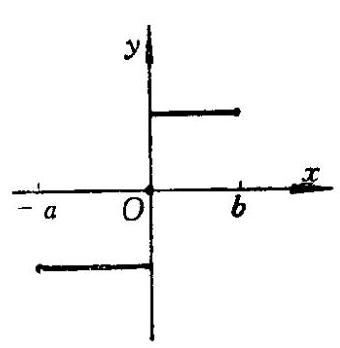
\includegraphics[max width=0.3\textwidth]{images/bo_d25ksc77aajc738obdgg_199_236_1182_340_348_0.jpg}
\end{center}
\hspace*{3em} 

\begin{center}
	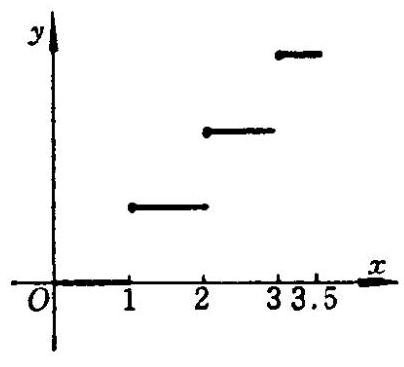
\includegraphics[max width=0.3\textwidth]{images/bo_d25ksc77aajc738obdgg_199_610_1163_404_367_0.jpg}
\end{center}
\hspace*{3em} 

\begin{center}
	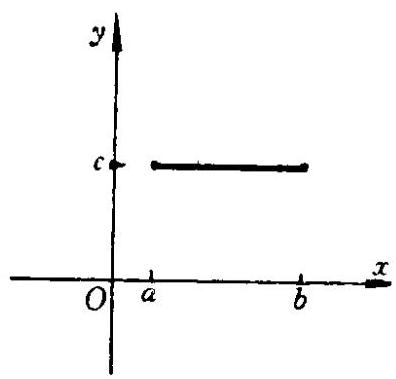
\includegraphics[max width=0.3\textwidth]{images/bo_d25ksc77aajc738obdgg_199_1054_1165_396_379_0.jpg}
\end{center}
\hspace*{3em} 

图 5-1

附注 适合于阶梯函数 $f$ 的二元组 $\left\lbrack  {\sigma ,\xi }\right\rbrack$ 不是唯一的. 例如若 $\left\lbrack  {\sigma ,\xi }\right\rbrack   = \left\lbrack  {{a}_{0},{a}_{1},\cdots ,{a}_{n};{c}_{0},{c}_{1},\cdots ,{c}_{n - 1}}\right\rbrack$ 适合于阶梯函数 $f$ ,则在 $\rbrack {a}_{i},{a}_{i + 1}\lbrack$ 上任意加入一个分点 $\bar{x}$ 后,我们得到 $\left\lbrack  {a,b}\right\rbrack$ 的另一个分割 ${\sigma }^{\prime } = \left( {{a}_{0},{a}_{1},\cdots ,{a}_{i},\bar{x},{a}_{i + 1},\cdots ,{a}_{n}}\right)$ 及另一个向量 ${\xi }^{\prime } = \left\lbrack  {{c}_{0},{c}_{1},\cdots ,}\right.$  $\left. {{c}_{i},{c}_{i},{c}_{i + 1},\cdots ,{c}_{n - 1}}\right\rbrack$ 满足
\begin{align*}
	&f\left( x\right)  = {c}_{k}\;\forall x \in  \rbrack {a}_{k},{a}_{k + 1}\lbrack ,k = 0,1,\cdots ,i - 1,i + 1,\cdots ,n - 1,\\
	&f\left( x\right)  = {c}_{i}\;\forall x \in  \rbrack {a}_{i},\bar{x}\left\lbrack  \bigcup \right\rbrack  \bar{x},{a}_{i + 1}\lbrack .
\end{align*}

因此 $\left\lbrack  {{\sigma }^{\prime },{\xi }^{\prime }}\right\rbrack$ 也适合于 $f$ 。

另一方面,如果分割 $\sigma  = \left( {{a}_{0},{a}_{1},\cdots ,{a}_{n},\cdots ,{a}_{n}}\right)$ 的分点 ${a}_{i}$ 满足 ${c}_{i - 1} = {c}_{i} = f\left( {a}_{i}\right)$ ,则删去 $\sigma$ 的分点 ${a}_{i}$ 后得到 $\left\lbrack  {a,b}\right\rbrack$ 的另一分割 ${\sigma }^{\prime \prime }$  $= \left( {{a}_{0},{a}_{1},\cdots ,{a}_{i - 1},{a}_{i + 1},\cdots ,{a}_{n}}\right)$ 及另一向量 ${\xi }^{\prime \prime } = \left\lbrack  {{c}_{0},{c}_{1},\cdots }\right.$ , $\left. {{c}_{i - 1},{c}_{i + 1},\cdots ,{c}_{n - 1}}\right\rbrack$ 满足
\begin{align*}
	&f\left( x\right)  = {c}_{k},\;\forall x \in  \rbrack {a}_{k},{a}_{k + 1}\lbrack ,\\
	&k = 0,1,\cdots ,i - 2,i + 1,\cdots ,n - 1,\\
	&f\left( x\right)  = {c}_{i},\;\forall x \in  \rbrack {a}_{i - 1},{a}_{i + 1}\lbrack .
\end{align*}

因此 $\left\lbrack  {{\sigma }^{\prime \prime },{\xi }^{\prime \prime }}\right\rbrack$ 也适合于 $f$ .

引理 设 $f : \left\lbrack  {a,b}\right\rbrack   \rightarrow  \mathbf{R}$ 是任一阶梯函数, $\left\lbrack  {\sigma ,\xi }\right\rbrack$ 适合于 $f$ , ${\sigma }^{\prime }$ 是 $\left\lbrack  {a,b}\right\rbrack$ 的任一分割,则存在向量 $\eta$ 使得 $\left\lbrack  {\sigma  \smallsetminus  {\sigma }^{\prime },\eta }\right\rbrack$ 适合于 $f$ .

证明 设 $\left\lbrack  {\sigma ,\xi }\right\rbrack   = \left\lbrack  {{a}_{0},{a}_{1},\cdots ,{a}_{n};{c}_{0},{c}_{1},\cdots ,{c}_{n - 1}}\right\rbrack$ . 由于 $\sigma  \vee  {\sigma }^{\prime }$ 也是 $\left\lbrack  {a,b}\right\rbrack$ 的一个分割,故若令
$$\sigma  \vee  {\sigma }^{\prime } = \left( {{b}_{0},{b}_{1},\cdots ,{b}_{m}}\right) ,$$

则 $\forall i = 0,1,\cdots ,m - 1$ ,存在 $j\left( i\right)  \in  \{ 0,1,\cdots ,n - 1\}$ 使得 $\rbrack {b}_{i},{b}_{i + 1}\left\lbrack   \subset  \right\rbrack  {a}_{j\left( i\right) },{a}_{j\left( i\right)  + 1}\lbrack$ ,于是
$$f\left( x\right)  = {c}_{j\left( i\right) },\;\forall x \in  \rbrack {b}_{i},{b}_{i + 1}\lbrack ,\forall i = 0,1,\cdots ,m - 1.$$

令 ${d}_{i} = {c}_{j\left( i\right) }\left( {i = 0,1,\cdots ,m - 1}\right)$ 及 $\eta  = \left\lbrack  {{d}_{0},{d}_{1},\cdots ,{d}_{m - 1}}\right\rbrack$ ,则 $\left\lbrack  {\sigma  \vee  {\sigma }^{\prime },\eta }\right\rbrack$ 适合于 $f$ .

命题 设 $f : \left\lbrack  {a,b}\right\rbrack   \rightarrow  \mathbf{R}$ 是任一阶梯函数, $\left\lbrack  {\sigma ,\xi }\right\rbrack   = \left\lbrack  {{a}_{0},{a}_{1}}\right.$ , $\cdots ,{a}_{n};{c}_{0},{c}_{1},\cdots ,{c}_{n - 1}\rbrack$ 与 $\left\lbrack  {{\sigma }^{\prime },{\xi }^{\prime }}\right\rbrack   = \left\lbrack  {{a}_{0}^{\prime },{a}_{1}^{\prime },\cdots ,{a}_{m}^{\prime };{c}_{0}^{\prime },{c}_{1}^{\prime },\cdots }\right.$ , $\left. {c}_{m - 1}^{\prime }\right\rbrack$ 都适合于 $f$ ,则
$$\mathop{\sum }\limits_{{i = 0}}^{{n - 1}}{c}_{i}\left( {{a}_{i + 1} - {a}_{i}}\right)  = \mathop{\sum }\limits_{{j = 0}}^{{m - 1}}{c}_{j}^{\prime }\left( {{a}_{j + 1}^{\prime } - {a}_{j}^{\prime }}\right) .$$

证明 我们记
\begin{align*}
	&I\left\lbrack  {\sigma ,\xi }\right\rbrack   = \mathop{\sum }\limits_{{i = 0}}^{{n - 1}}{c}_{i}\left( {{a}_{i + 1} - {a}_{i}}\right) ,\\
	&I\left\lbrack  {{\sigma }^{\prime },{\xi }^{\prime }}\right\rbrack   = \mathop{\sum }\limits_{{j = 0}}^{{m - 1}}{c}_{j}^{\prime }\left( {{a}_{j + 1}^{\prime } - {a}_{j}^{\prime }}\right) .
\end{align*}

根据引理,存在一个向量 $\eta$ 使得 $\left\lbrack  {\sigma \bigvee {\sigma }^{\prime },\eta }\right\rbrack$ 适合于 $f$ . 只需要证明
$$I\left\lbrack  {\sigma ,\xi }\right\rbrack   = I\left\lbrack  {\sigma  \vee  {\sigma }^{\prime },\eta }\right\rbrack   = I\left\lbrack  {{\sigma }^{\prime },{\xi }^{\prime }}\right\rbrack  .$$

我们首先假设 $\sigma  \smallsetminus  {\sigma }^{\prime }$ 比 $\sigma$ 多一个分点 $\bar{x}$ . 令 $\bar{x} \in  \rbrack {a}_{i},{a}_{i + 1}\lbrack$ . 那未
\begin{align*}
	&\sigma  \vee  {\sigma }^{\prime } = \left( {{a}_{0},{a}_{1},\cdots ,{a}_{i},\bar{x},{a}_{i + 1},\cdots ,{a}_{n}}\right) ,\\
	&\eta  = \left\lbrack  {{c}_{0},{c}_{1},\cdots ,{c}_{i},{c}_{i},{c}_{i + 1},\cdots ,{c}_{n - 1}}\right\rbrack  ,
\end{align*}

于是
\begin{align*}
	&I\left\lbrack  {\sigma  \vee  {\sigma }^{\prime },\eta }\right\rbrack   = {c}_{0}\left( {{a}_{1} - {a}_{0}}\right)  + {c}_{1}\left( {{a}_{2} - {a}_{1}}\right)  + \cdots  + {c}_{i}\left( {\bar{x} - {a}_{i}}\right)\\
	&+ {c}_{i}\left( {{a}_{i + 1} - \bar{x}}\right)  + \cdots  + {c}_{n - 1}\left( {{a}_{n} - {a}_{n - 1}}\right)\\
	&= {c}_{0}\left( {{a}_{1} - {a}_{0}}\right)  + {c}_{1}\left( {{a}_{2} - {a}_{1}}\right)  + \cdots  + {c}_{i}\left( {{a}_{i + 1} - {a}_{i}}\right)\\
	&+ \cdots  + {c}_{n - 1}\left( {{a}_{n} - {a}_{n - 1}}\right)\\
	&= I\left\lbrack  {\sigma ,\xi }\right\rbrack  \text{ . }
\end{align*}

对一般的 $\sigma$ 与 ${\sigma }^{\prime }$ ,由于 $\sigma  \smallsetminus  {\sigma }^{\prime }$ 可以通过在 $\sigma$ 上逐步添加 ${\sigma }^{\prime }$ 的分点的方法来得到,故由归纳法我们有 $I\left\lbrack  {\sigma  \vee  {\sigma }^{\prime },\eta }\right\rbrack   = I\left\lbrack  {\sigma ,\xi }\right\rbrack$ .

同理,存在向量 ${\eta }^{\prime }$ 使得 $\left\lbrack  {{\sigma }^{\prime } \vee  \sigma ,{\eta }^{\prime }}\right\rbrack$ 也适合于 $f$ ,并且 $I\left\lbrack  {{\sigma }^{\prime } \vee  \sigma }\right.$ , $\left. {\eta }^{\prime }\right\rbrack   = I\left\lbrack  {{\sigma }^{\prime },{\xi }^{\prime }}\right\rbrack$ .

由于 $\sigma  \smallsetminus  /{\sigma }^{\prime } = {\sigma }^{\prime } \smallsetminus  /\sigma$ ,故 $\eta  = {\eta }^{\prime }$ . 因此 $\mathbf{I}\left\lbrack  {\sigma  \smallsetminus  /{\sigma }^{\prime },\eta }\right\rbrack   = \mathbf{I}\left\lbrack  {{\sigma }^{\prime } \smallsetminus  /\sigma }\right.$ , $\left. {\eta }^{\prime }\right\rbrack$ ,从而 $I\left\lbrack  {\sigma ,\eta }\right\rbrack   = I\left\lbrack  {\sigma  \vee  {\sigma }^{\prime },\eta }\right\rbrack   = I\left\lbrack  {{\sigma }^{\prime },{\xi }^{\prime }}\right\rbrack$ .

上述命题表明, $I\left\lbrack  {\sigma ,\xi }\right\rbrack$ 是一个只与 $f$ 有关而与适合于 $f$ 的二元组 $\left\lbrack  {\sigma ,\xi }\right\rbrack$ 的选择无关的定数. 因此我们可以引入下述定义.

定义 设 $f : \left\lbrack  {a,b}\right\rbrack   \rightarrow  \mathbf{R}$ 是任一阶梯函数, $\left\lbrack  {\sigma ,\xi }\right\rbrack   = \left\lbrack  {{a}_{0},{a}_{1}}\right.$ , $\cdots ,{a}_{n};{c}_{0},{c}_{1},\cdots ,{c}_{n - 1}\rbrack$ 适合于 $f$ . 则实数
$$I\left( f\right)  = {c}_{0}\left( {{a}_{1} - {a}_{0}}\right)  + {c}_{1}\left( {{a}_{2} - {a}_{1}}\right)  + \cdots  + {c}_{n - 1}\left( {{a}_{n} - {a}_{n - 1}}\right)$$

称为 $f$ 在 $\left\lbrack  {a,b}\right\rbrack$ 上的积分,记为 ${\int }_{a}^{b}f\left( x\right) {dx}$ . 于是
$${\int }_{a}^{b}f\left( x\right) {dx} = \mathop{\sum }\limits_{{i = 0}}^{{n - 1}}{c}_{i}\left( {{a}_{i + 1} - {a}_{i}}\right) .$$

例 $4\forall c \in  \mathbf{R}$ ,常值函数 $x \mapsto  c,x \in  \left\lbrack  {a,b}\right\rbrack  \left( {a < b}\right)$ 的积分
$${\int }_{a}^{b}{cdx} = c\left( {b - a}\right) .$$

例 5 符号函数 $x \mapsto  \operatorname{sgn}\left( x\right) ,x \in  \left\lbrack  {a,b}\right\rbrack  \left( {a < b}\right)$ 的积分
$${\int }_{a}^{b}\operatorname{sgn}\left( x\right) {dx} = \left\{  \begin{array}{ll} b - a, & \text{ 若 }0 \leq  a < b, \\  a + b, & \text{ 若 }a < 0 < b, \\  a - b, & \text{ 若 }a < b \leq  0. \end{array}\right.$$

从阶梯函数积分的定义可知,积分值 ${\int }_{a}^{b}f\left( x\right) {dx}$ 与 $f$ 在分点 ${a}_{i}$ 的值 $f\left( {a}_{i}\right) \left( {i = 0,1,\cdots ,n}\right)$ 无关. 因此改变阶梯函数 $f$ 在分点 ${a}_{i}$ 的值所得新的阶梯函数 $g$ 与 $f$ 在 $\left\lbrack  {a,b}\right\rbrack$ 上有相同的积分值.

从几何上看,阶梯函数 $f$ 的积分 ${\int }_{a}^{b}f\left( x\right) {dx}$ 表示在平面直角坐标系 $\left\{  {0;x,y}\right\}$ 的 $x$ 轴上以 $\left\lbrack  {{a}_{i},{a}_{i + 1}}\right\rbrack$ 为底边,以 ${c}_{i}$ 为 “高” 的长方形”面积”的代数和.

\begin{center}
	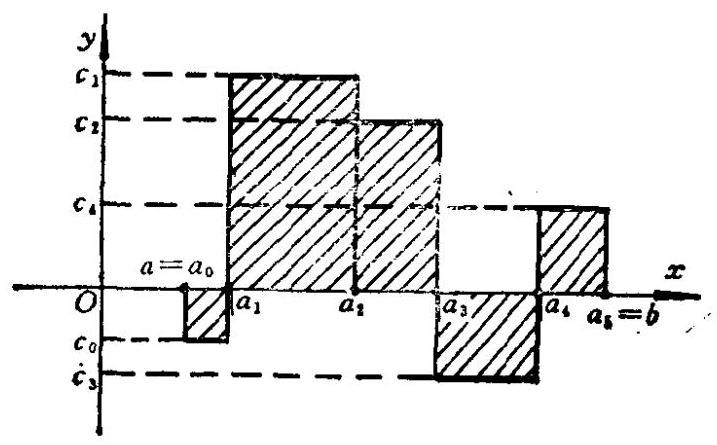
\includegraphics[max width=0.6\textwidth]{images/bo_d25ksc77aajc738obdgg_202_355_1142_717_445_0.jpg}
\end{center}
\hspace*{3em} 

图 5-2

\section*{3. 阶梯函数积分的性质}

我们用 $\mathcal{E}\left\lbrack  {a,b}\right\rbrack$ 表示所有定义在 $\left\lbrack  {a,b}\right\rbrack$ 上的阶梯函数的集合.

定理 $5 \cdot  1 \cdot  1$ 设 $f,g \in  \mathcal{E}\left\lbrack  {a,b}\right\rbrack  ,\alpha ,\beta  \in  \mathbf{R}$ ,则

1) ${\alpha f} + {\beta g} \in  \mathcal{E}\left\lbrack  {a,b}\right\rbrack$ ,并且
$${\int }_{a}^{b}\left\lbrack  {{\alpha f} + {\beta g}}\right\rbrack  \left( x\right) {dx} = \alpha {\int }_{a}^{b}f\left( x\right) {dx} + \beta {\int }_{a}^{b}g\left( x\right) {dx}.$$

2) 若 $f \geq  0$ ,则 ${\int }_{a}^{b}f\left( x\right) {dx} \geq  0$ .

3) 若 $f \geq  g$ ,则 ${\int }_{a}^{b}f\left( x\right) {dx} > {\int }_{a}^{b}g\left( x\right) {dx}$ .

4) $\left| f\right|  \in  \mathcal{E}\left\lbrack  {a,b}\right\rbrack$ ,并且 $\left| {{\int }_{a}^{b}f\left( x\right) {dx}}\right|  \leq  {\int }_{a}^{b}\left| {f\left( x\right) }\right| {dx}$ .

证明 1) 设 $\left\lbrack  {\sigma ,\xi }\right\rbrack$ 与 $\left\lbrack  {{\sigma }^{\prime },{\xi }^{\prime }}\right\rbrack$ 分别适合于 $f$ 与 $g$ . 令 $\sigma  \vee  {\sigma }^{\prime }$  $= \left( {{a}_{0},{a}_{1},\cdots ,{a}_{n}}\right)$ . 由引理知存在两个向量
$$\eta  = \left\lbrack  {{c}_{0},{c}_{1},\cdots ,{c}_{n - 1}}\right\rbrack  ,\zeta  = \left\lbrack  {{d}_{0},{d}_{1},\cdots ,{d}_{n - 1}}\right\rbrack  ,$$

使得 $\left\lbrack  {\sigma  \vee  {\sigma }^{\prime },\eta }\right\rbrack$ 与 $\left\lbrack  {\sigma  \vee  {\sigma }^{\prime },\zeta }\right\rbrack$ 分别适合于 $f$ 与 $g$ .

若令
$${a\eta } + {\beta \zeta } = \left\lbrack  {\alpha {c}_{0} + \beta {d}_{0},\alpha {c}_{1} + \beta {d}_{1},\cdots ,\alpha {c}_{n - 1} + \beta {d}_{n - 1}}\right\rbrack  ,$$

则 $\left\lbrack  {\sigma  \vee  {\sigma }^{\prime },{\alpha \eta } + {\beta \zeta }}\right\rbrack$ 适合于 ${\alpha f} + {\beta g}$ ,因此 ${\alpha f} + {\beta g} \in  \mathcal{E}\left\lbrack  {a,b}\right\rbrack$ . 由阶梯函数积分定义, 我们有
\begin{align*}
	&{\int }_{a}^{b}\left\lbrack  {{\alpha f} + {\beta g}}\right\rbrack  \left( x\right) {dx} = \mathop{\sum }\limits_{{i = 0}}^{{n - 1}}\left( {\alpha {c}_{i} + \beta {d}_{i}}\right) \left( {{a}_{i + 1} - {a}_{i}}\right)\\
	&= \alpha \mathop{\sum }\limits_{{i = 0}}^{{n - 1}}{c}_{i}\left( {{a}_{i + 1} - {a}_{i}}\right)  + \beta \mathop{\sum }\limits_{{i = 0}}^{{n - 1}}{d}_{i}\left( {{a}_{i + 1} - {a}_{i}}\right)\\
	&= \alpha {\int }_{a}^{b}f\left( x\right) {dx} + \beta {\int }_{a}^{b}g\left( x\right) {dx}.
\end{align*}

2) 若 $f \geq  0$ ,则 ${c}_{i} \geq  0\left( {i = 0,1,\cdots ,n - 1}\right)$ ,因此
$${\int }_{a}^{b}f\left( x\right) {dx} = \mathop{\sum }\limits_{{i = 0}}^{{n - 1}}{c}_{i}\left( {{a}_{i + 1} - {a}_{i}}\right)  \geq  0.$$

3) 若 $f \geq  g$ ,则 ${c}_{i} \geq  {d}_{i}\left( {i = 0,1,2,\cdots ,n - 1}\right)$ 因此
\begin{align*}
	&{\int }_{a}^{b}f\left( x\right) {dx} = \mathop{\sum }\limits_{{i = 0}}^{{n - 1}}{c}_{i}\left( {{a}_{i + 1} - {a}_{i}}\right)  \geq  \mathop{\sum }\limits_{{i = 0}}^{{n - 1}}{d}_{i}\left( {{a}_{i + 1} - {a}_{i}}\right)\\
	&= {\int }_{a}^{b}g\left( x\right) {dx}.
\end{align*}

4)令
$$\left| \eta \right|  = \left\lbrack  {\left| {c}_{0}\right| ,\left| {c}_{1}\right| ,\cdots ,\left| {c}_{n - 1}\right| }\right\rbrack  ,$$

则 $\left\lbrack  {\sigma  \smallsetminus  {\sigma }^{\prime },\left| \eta \right| }\right\rbrack$ 适合于 $\left| f\right|$ ,因此 $\left| f\right|  \in  \mathcal{E}\left\lbrack  {a,b}\right\rbrack$ ,并且
\begin{align*}
	&\left| {{\int }_{a}^{b}f\left( x\right) {dx}}\right|  = \left| {\mathop{\sum }\limits_{{i = 0}}^{{n - 1}}{c}_{i}\left( {{a}_{i + 1} - {a}_{i}}\right) }\right|  \leq  \mathop{\sum }\limits_{{i = 0}}^{{n - 1}}\left| {c}_{i}\right| \left( {{a}_{i + 1} - {a}_{i}}\right)\\
	&= {\int }_{a}^{b}\left| {f\left( x\right) }\right| {dx}.
\end{align*}

现在设 $f : \left\lbrack  {a,b}\right\rbrack   \rightarrow  \mathbf{R}$ 是任一阶梯函数. 我们作下述约定:
$${\int }_{a}^{a}f\left( x\right) {dx} = 0,{\int }_{b}^{b}f\left( x\right) {dx} = 0.$$

定理 $5 \cdot  1 \cdot  2$ 设 $f \in  \mathcal{E}\left\lbrack  {a,b}\right\rbrack$ ,则 $\forall c \in  \left\lbrack  {a,b}\right\rbrack$ ,
\begin{align*}
	&{\left. f\right| }_{\left\lbrack  a;c\right\rbrack  } \in  \mathcal{E}\left\lbrack  {a,c}\right\rbrack  ,{\left. f\right| }_{\left\lbrack  c,b\right\rbrack  } \in  \mathcal{E}\left\lbrack  {c,b}\right\rbrack  \text{ 并且 }\\
	&{\int }_{a}^{b}f\left( x\right) {dx} = {\int }_{a}^{c}{\left. f\right| }_{\left\lbrack  a,c\right\rbrack  }\left( x\right) {dx} + {\int }_{c}^{b}{\left. f\right| }_{\left\lbrack  c,b\right\rbrack  }\left( x\right) {dx}.
\end{align*}

证明 设 $\left\lbrack  {\sigma ,\xi }\right\rbrack   = \left\lbrack  {{a}_{0},{a}_{1},\cdots ,{a}_{n};{c}_{0},{c}_{1},\cdots ,{c}_{n - 1}}\right\rbrack$ 适合于 $f$ . 令 $c \in  \left\lbrack  {{a}_{{i}_{0}},{a}_{{i}_{0} + 1}}\right\rbrack$ .

不妨设 $c \in  \rbrack a,b\lbrack$ ,因为若 $c = a$ 或 $c = b$ ,则根据上述约定,定理显然成立.

1) 若 $c = {a}_{{i}_{0}}$ ,则存在 $\left\lbrack  {a,c}\right\rbrack$ 的一个分割 ${\sigma }_{1} = \left( {{a}_{0},{a}_{1},\cdots ,{a}_{{i}_{0}}}\right)$ 及相应向量 ${\xi }_{1} = \left\lbrack  {{c}_{0},{c}_{1},\cdots ,{c}_{{i}_{0} - 1}}\right\rbrack  \text{ 、 }\left\lbrack  {c,b}\right\rbrack$ 的一个分割 ${\sigma }_{2} = \left\lbrack  {a}_{{i}_{0}}\right.$ , $\left. {{a}_{{i}_{0} + 1},\cdots ,{a}_{n}}\right)$ 及相应向量 ${\xi }_{2} = \left\lbrack  {{c}_{{i}_{0}},{c}_{{i}_{0} + 1},\cdots ,{c}_{n - 1}}\right\rbrack$ 使得
\begin{align*}
	&{\left. f\right| }_{\left\lbrack  a,c\right\rbrack  }\left( x\right)  = {c}_{i},\forall x \in  \rbrack {a}_{i},{a}_{i + 1}\lbrack ,\;i = 0,1,\cdots ,{i}_{0} - 1,\\
	&{\left. f\right| }_{\left\lbrack  c,b\right\rbrack  }\left( x\right)  = {c}_{i},\;\forall x \in  \rbrack {a}_{i},{a}_{i + 1}\left\lbrack  {\;i = {i}_{0},{i}_{0} + 1,\cdots ,n - 1.}\right.
\end{align*}

因此 $\left\lbrack  {{\sigma }_{1},{\xi }_{1}}\right\rbrack$ 适合于 $f{|}_{\left\lbrack  a,c\right\rbrack  },\left\lbrack  {{\sigma }_{2},{\xi }_{2}}\right\rbrack$ 适合于 $f{|}_{\left\lbrack  c,b\right\rbrack  }$ . 从而 ${\left. f\right| }_{\left\lbrack  a,c\right\rbrack  } \in  \mathcal{E}\left\lbrack  {a,c}\right\rbrack  ,{\left. f\right| }_{\left\lbrack  c,b\right\rbrack  } \in  \mathcal{E}\left\lbrack  {c,b}\right\rbrack$ ,并且由积分定义有
\begin{align*}
	&{\int }_{a}^{b}f\left( x\right) {dx} = \mathop{\sum }\limits_{{i = 0}}^{{n - 1}}{c}_{i}\left( {{a}_{i + 1} - {a}_{i}}\right)\\
	&= \mathop{\sum }\limits_{{i = 0}}^{{{i}_{0} - 1}}{c}_{i}\left( {{a}_{i + 1} - {a}_{i}}\right)  + \mathop{\sum }\limits_{{i = 1}}^{{n - 1}}{c}_{i}\left( {{a}_{i + 1} - {a}_{i}}\right)\\
	&= {\int }_{a}^{c}f{\left| {}_{\left\lbrack  a,c\right\rbrack  }\left( x\right) dx + {\int }_{c}^{b}f\right| }_{\left\lbrack  c,b\right\rbrack  }\left( x\right) {dx}.
\end{align*}

2) 若 $c \in  \rbrack {a}_{{i}_{0}},{a}_{{i}_{0} + 1}\lbrack$ ,则存在 $\left\lbrack  {a,c}\right\rbrack$ 的一个分割 ${\sigma }_{1} = \left( {a}_{0}\right.$ , $\left. {{a}_{1},\cdots ,{c}_{{i}_{0}},c}\right)$ 及相应向量 ${\xi }_{1} = \left\lbrack  {{c}_{0},{c}_{1},\cdots ,{c}_{{i}_{0}}}\right\rbrack  \text{ 、 }\left\lbrack  {c,b}\right\rbrack$ 的一个分割 ${\sigma }_{2} = \left( {c,{a}_{{i}_{0} + 1},\cdots ,{a}_{n}}\right)$ 及相应向量 ${\xi }_{2} = \left\lbrack  {{c}_{{i}_{0}},{c}_{{i}_{0} + 1},\cdots ,{c}_{n - 1}}\right\rbrack$ 使得
\begin{align*}
	&{\left. f\right| }_{\left\lbrack  a,c\right\rbrack  }\left( x\right)  = {c}_{i},\;\forall x \in  \rbrack {a}_{i},{a}_{i + 1}\lbrack ,i = 0,1,\cdots ,{i}_{0} - 1,\\
	&{\left. f\right| }_{\left\lbrack  a,c\right\rbrack  }\left( x\right)  = {c}_{{i}_{0}},\;\forall x \in  \rbrack {a}_{{i}_{0}},c\lbrack ,\\
	&{\left. f\right| }_{\left\lbrack  c,b\right\rbrack  }\left( x\right)  = {c}_{i},\forall x \in  \rbrack {a}_{i},{a}_{i + 1}\left\lbrack  {,i = {i}_{0} + 1,{i}_{0} + 2,\cdots ,n - 1,}\right.\\
	&{\left. f\right| }_{\left\lbrack  c,b\right\rbrack  }\left( x\right)  = {c}_{{i}_{0}},\;\forall x \in  \rbrack c,{a}_{{i}_{0} + 1}\lbrack .
\end{align*}

因此 $\left\lbrack  {{\sigma }_{1},{\xi }_{1}}\right\rbrack$ 适合于 ${\left. f\right| }_{\left\lbrack  a,c\right\rbrack  },\left\lbrack  {{\sigma }_{2},{\xi }_{2}}\right\rbrack$ 适合于 ${\left. f\right| }_{\left\lbrack  c,b\right\rbrack  }$ ,从而 ${\left. f\right| }_{\left\lbrack  a,c\right\rbrack  } \in  \mathcal{E}\left\lbrack  {a,c}\right\rbrack  ,{\left. f\right| }_{\left\lbrack  c,b\right\rbrack  } \in  \mathcal{E}\left\lbrack  {c,b}\right\rbrack$ ,并且
\begin{align*}
	&{\int }_{a}^{b}f\left( x\right) {dx} = \mathop{\sum }\limits_{{i = 0}}^{{n - 1}}{c}_{i}\left( {{a}_{i + 1} - {a}_{i}}\right)\\
	&= \mathop{\sum }\limits_{{i = 0}}^{{{i}_{0} - 1}}{c}_{i}\left( {{a}_{i + 1} - {a}_{i}}\right)  + {c}_{{i}_{0}}\left( {{a}_{{i}_{0} + 1} - {a}_{{i}_{0}}}\right)\\
	&+ \mathop{\sum }\limits_{{i = i}}^{{n - 1}}{c}_{i}\left( {{a}_{i + 1} - {a}_{i}}\right)\\
	&= \mathop{\sum }\limits_{{i = 0}}^{{{i}_{0} - 1}}{c}_{i}\left( {{a}_{i + 1} - {a}_{i}}\right)  + {c}_{{i}_{0}}\left( {c - {a}_{{i}_{0}}}\right)\\
	&+ {c}_{{i}_{0}}\left( {{a}_{{i}_{0} + 1} - c}\right)  + \mathop{\sum }\limits_{{i = {i}_{0} + 1}}^{{n - 1}}{c}_{i}\left( {{a}_{i + 1} - {a}_{i}}\right)\\
	&= {\int }_{a}^{c}f{\left| {}_{\left\lbrack  a,c\right\rbrack  }\left( x\right) dx + {\int }_{c}^{b}f\right| }_{\left\lbrack  c,b\right\rbrack  }\left( x\right) {dx}.
\end{align*}

为简单起见,今后一律用 ${\int }_{a}^{c}f\left( x\right) {dx}$ 表示 ${\int }_{a}^{c}f{|}_{\left\lbrack  a,c\right\rbrack  }\left( x\right) {dx}$ ,

用 ${\int }_{c}^{b}f\left( x\right) {dx}$ 表示 ${\int }_{c}^{b}f{|}_{\left\lbrack  c,b\right\rbrack  }\left( x\right) {dx}$ .

\section*{习 题}

1. 考虑如下定义的函数 $f : \left\lbrack  {0,1}\right\rbrack   \rightarrow  \mathbf{R}$ :
$$f\left( x\right)  = \frac{1}{n},\;\forall x \in  \left\rbrack  {\frac{1}{n + 1}\;\frac{1}{n}}\right\rbrack  \;\left( {\forall n \in  \mathbf{N}}\right) .$$

$f$ 是 $\left\lbrack  {0,1}\right\rbrack$ 上的阶梯函数吗?

2. 只取有限个值的函数 $f : \left\lbrack  {a,b}\right\rbrack   \rightarrow  R$ 一定是阶梯函数吗? 考虑定义在 $\left\lbrack  {a,b}\right\rbrack$ 上的Dirichlet函数
$$x \mapsto  D\left( x\right)  = \left\{  \begin{array}{ll} 1, & x \in  \left\lbrack  {a,b}\right\rbrack   \cap  {Q}_{3} \\  0, & x \in  \left\lbrack  {a,b}\right\rbrack   \cap  {Q}^{c}. \end{array}\right.$$

3. 设 $f,g \in  \mathcal{E}\left\lbrack  {a,b}\right\rbrack$ . 证明: ${fg} \in  \mathcal{E}\left\lbrack  {a,b}\right\rbrack$ ; 若 $g \neq  0$ ,则 $\frac{f}{g} \in  \mathcal{E}\left\lbrack  {a,b}\right\rbrack$ .

4. 设 $f \in  g\left\lbrack  {a,b}\right\rbrack  ,g : \left\lbrack  {c,d}\right\rbrack   \rightarrow  \mathrm{R}$ 是任一函数,且 $f\left( \left\lbrack  {a,b}\right\rbrack  \right)  \subset  \lbrack c$ , $d\rbrack$ . 证明: 复合函数 $g \circ  f \in  \mathcal{E}\left\lbrack  {a,b}\right\rbrack$ .

5. 设 $f \in  g\left\lbrack  {a,b}\right\rbrack  ,\forall M \in  R$ ,我们定义 ${f}^{ * } : \left\lbrack  {a,b}\right\rbrack   \rightarrow  R$ 如下:
$${f}^{ * }\left( x\right)  = \left\{  {\begin{array}{ll} f\left( x\right) , & \text{ 若 }f\left( x\right)  \leq  M, \\  M, & \text{ 若 }f\left( x\right)  > M, \end{array}\;\forall x \in  \left\lbrack  {a,b}\right\rbrack  .}\right.$$

证明: ${f}^{ * } \in  g\left\lbrack  {a,b}\right\rbrack$ ,并且 ${f}^{ * } \leq  f$ .

6. 设 $f,g \in  \mathcal{E}\left\lbrack  {a,b}\right\rbrack$ ,定义函数 $m,M : \left\lbrack  {a,b}\right\rbrack   \rightarrow  \mathbf{R}$ 如下:
\begin{align*}
	&m\left( x\right)  = \min \left( {f\left( x\right) ,g\left( x\right) }\right) ,M\left( x\right)  = \max \left( {f\left( x\right) ,g\left( x\right) }\right) ,\\
	&\forall x \in  \left\lbrack  {a,b}\right\rbrack  .
\end{align*}

证明: $m,M \in  \mathcal{E}\left\lbrack  {a,b}\right\rbrack$ . 特别地若令 ${f}^{ + },{f}^{ - } : \left\lbrack  {a,b}\right\rbrack   \rightarrow  R$ 为
$${f}^{ + }\left( x\right)  = \max \left( {f\left( x\right) ,0}\right) ,{f}^{ - }\left( x\right)  = \max \left( {-f\left( x\right) ,0}\right) ,\forall x \in  \left\lbrack  {a,b}\right\rbrack  ,$$

则 ${f}^{ + },{f}^{ - } \in  \mathcal{E}\left\lbrack  {a,b}\right\rbrack$ ,并且 ${f}^{ + } \geq  0,{f}^{ - } \geq  0,f = {f}^{ + } - {f}^{ - }$ .

\section{Riemann可积函数}

现在我们来介绍一般一元实值函数的Riemann积分理论.

\section*{1. 问题的提出}

设 $f : \left\lbrack  {a,b}\right\rbrack   \rightarrow  \mathrm{R}$ 是任一有界正函数. 我们用 $G$ 表示平面上由

直线 $x = a,x = b,x$ 轴以及 $f$ 的曲线 $\Gamma$ 所围的 “曲边梯形”.

\begin{center}
	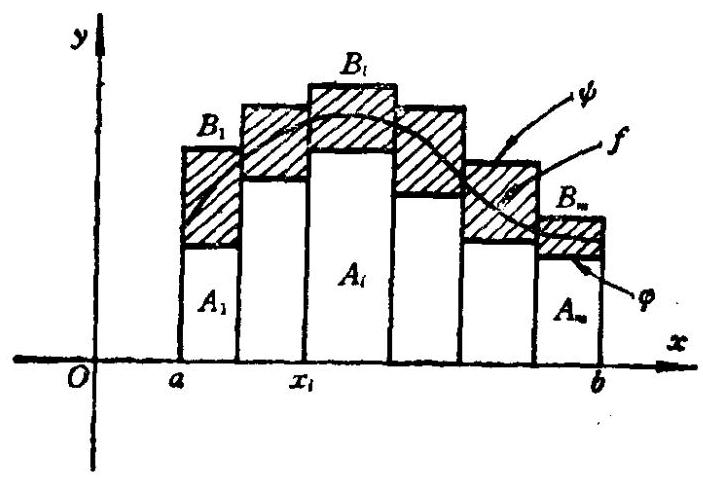
\includegraphics[max width=0.6\textwidth]{images/bo_d25ksc77aajc738obdgg_207_515_349_703_480_0.jpg}
\end{center}
\hspace*{3em} 

图 5-3

对于这样的一个曲 边梯形 $G$ ,当 $\Gamma$ 不是一条线段时,如何定义 $G$ 是可求 “面积”的？又如何定义 $G$ 的 “面积”！这是我们非常关心的一个实际问题. 很自然的一个想法就是: 用若干直 线 $x = {x}_{i}$  $\left( {a \leq  {x}_{i} \leq  b}\right)$ 去分割 $G$ 以得到若干个子曲边梯形 ${G}_{i}$ 例如
$$G = {G}_{1} \cup  {G}_{2} \cup  \cdots  \cup  {G}_{m}.$$

对每一个 ${G}_{i}$ ,我们找两个长方形 ${A}_{i},{B}_{i}$ 使得 ${A}_{i} \subset  {G}_{i} \subset  {B}_{i}$  $\left( {i = 1,2,\cdots ,m}\right)$ . ${A}_{i}$ 与 ${B}_{i}$ 的面积,记为 $\left| {A}_{i}\right|$ 与 $\left| {B}_{i}\right|$ ,是我们会计算的.

现在我们可以想象的是: 如果对任意的 $\varepsilon  > 0$ ,可适当的分割 $G$ 为 $G = \mathop{\bigcup }\limits_{{i = 1}}^{m}{G}_{i}$ ,并且对每一个 ${G}_{i}$ 可适当地选择 ${A}_{i},{B}_{i}$ 使得
$$\mathop{\bigcup }\limits_{{i = 1}}^{m}{A}_{i} \subset  G \subset  \mathop{\bigcup }\limits_{{i = 1}}^{m}{B}_{i},\;0 \leq  \mathop{\sum }\limits_{{i = 1}}^{m}\left| {B}_{i}\right|  - \mathop{\sum }\limits_{{i = 1}}^{m}\left| {A}_{i}\right|  < \varepsilon ,$$

那末曲边梯形 $G$ 应该认为是可以求 “面积”的,并且可以把 $\mathop{\sum }\limits_{{i = 1}}^{m}\left| {A}_{i}\right|$ 或 $\mathop{\sum }\limits_{{i = 1}}^{m}\left| {B}_{i}\right|$ 当作 $G$ 的 “面积” 的近似值.

由于 $\mathop{\sum }\limits_{{i = 1}}^{m}\left| {A}_{i}\right|$ 与 $\mathop{\sum }\limits_{{i = 1}}^{m}\left| {B}_{i}\right|$ 实际上就是某两个阶梯函数 $\varphi  : \left\lbrack  {a,b}\right\rbrack$  $\rightarrow  \mathrm{R}$ 与 $\psi  : \left\lbrack  {a,b}\right\rbrack   \rightarrow  \mathrm{R}$ 的积分值,即 ${\int }_{a}^{b}\varphi \left( x\right) {dx} = \mathop{\sum }\limits_{{i = 1}}^{m}\left| {A}_{i}\right|$ ,

${\int }_{a}^{b}\psi \left( x\right) {dx} = \mathop{\sum }\limits_{{i = 1}}^{m}\left| {B}_{i}\right|$ ,故上面我们所说的 $G$ 是可求面积的,就等价于:

$\forall \varepsilon  > 0,\exists \varphi ,\psi  \in  \mathcal{E}\left\lbrack  {a,b}\right\rbrack$ 使得
$$\varphi \left( x\right)  \leq  f\left( x\right)  \leq  \psi \left( x\right) \;\forall x \in  \left\lbrack  {a,b}\right\rbrack  ,{\int }_{a}^{b}\left\lbrack  {\psi \left( x\right)  - \varphi \left( x\right) }\right\rbrack  {dx} < \bar{\varepsilon },$$

并且这时积分值 ${\int }_{a}^{b}\varphi \left( x\right) {dx}$ 或 ${\int }_{a}^{b}\psi \left( x\right) {dx}$ 就是 $G$ 的面积的近似值.

上述这种十分自然的想法就是我们下面要介绍的, 一般一元实值有界函数Riemann可积性概念的基础.

\section*{2. Riemann可积性定义}

定义 设 $\left\lbrack  {a,b}\right\rbrack$ 是任一有限闭区间, $f : \left\lbrack  {a,b}\right\rbrack   \rightarrow  \mathbf{R}$ 是任一函数,我们称 $f$ 在 $\left\lbrack  {a,b}\right\rbrack$ 上是Riemann可积的 (简称为可积),如果 $\forall \varepsilon  > 0,\exists \varphi ,\psi  \in  \mathcal{E}\left\lbrack  {a,b}\right\rbrack$ 使得
\begin{align*}
	&\varphi \left( x\right)  \leq  f\left( x\right)  \leq  \psi \left( x\right) ,\;\forall x \in  \left\lbrack  {a,b}\right\rbrack  ,\\
	&{\int }_{a}^{b}\left\lbrack  {\psi \left( x\right)  - \varphi \left( x\right) }\right\rbrack  {dx} < \varepsilon .
\end{align*}

因此从分析的角度来看,函数 $f$ 在 $\left\lbrack  {a,b}\right\rbrack$ 上Riemann可积,等价于: 可以分别从 $f$ 的上方与下方用阶梯函数 $\psi$ 与 $\varphi$ 来逼近 $f$ ,并且这两个阶梯函数 $\psi$ 与 $\varphi$ 在 $\left\lbrack  {a,b}\right\rbrack$ 上的积分之差 ${\int }_{a}^{b}\left\lbrack  {\psi \left( x\right)  - \varphi \left( x\right) }\right\rbrack  {dx}$ 能够任意的小.

例 1 任意一个阶梯 函数 $f : \left\lbrack  {a,b}\right\rbrack   \rightarrow  \mathbf{R}$ 在 $\left\lbrack  {a,b}\right\rbrack$ 上是 Rie- $\operatorname{mann可积的.}$

因为我们可以取 $\rho  = \psi  = f$ .

例2 Dirichlet函数
$$x \mapsto  D\left( x\right)  = \left\{  \begin{array}{l} 1,\text{ 若 }x \in  \left\lbrack  {a,b}\right\rbrack   \cap  \mathbf{Q}, \\  0,\text{ 若 }x \in  \left\lbrack  {a,b}\right\rbrack   \cap  {\mathbf{Q}}^{c}. \end{array}\right. \text{ 在 }\left\lbrack  {a,b}\right\rbrack  \text{ 上不是 }$$

Riemann可积的.

事实上,设 $\varphi ,\psi  \in  \mathcal{A}\left\lbrack  {a,b}\right\rbrack$ 并且满足不等式
$$\varphi \left( x\right)  \leq  D\left( x\right)  \leq  \psi \left( x\right) \;\forall x \in  \left\lbrack  {a,b}\right\rbrack  .$$

由 $§1$ 的 引理 1 知,存在 $\left\lbrack  {a,b}\right\rbrack$ 的一个分割 $\sigma  = \left( {{a}_{0},\cdots ,{a}_{n}}\right)$ 及两个向量 $\xi  = \left\lbrack  {{c}_{0},{c}_{1},\cdots ,{c}_{n - 1}}\right\rbrack  ,\eta  = \left\lbrack  {{d}_{0},{d}_{1},\cdots ,{d}_{n - 1}}\right\rbrack$ 使得 $\left\lbrack  {\sigma ,\xi }\right\rbrack$ 适合于 $\varphi ,\left\lbrack  {\sigma ,\eta }\right\rbrack$ 适合于 $\psi$ . 因此
\begin{align*}
	&\forall i = 0,1,\cdots ,n - 1,\;\forall x \in  \rbrack {a}_{i},{a}_{i + 1}\lbrack ,\\
	&{c}_{i} = \varphi \left( x\right)  \leq  D\left( x\right)  \leq  \psi \left( x\right)  = {d}_{i}
\end{align*}

但 $D\left( x\right)  = 1$ ,若 $x \in  \rbrack {a}_{i},{a}_{i + 1}\left\lbrack  {\cap \mathbf{Q};D\left( x\right)  = 0\text{ 若 }x \in  }\right\rbrack  {a}_{i},{a}_{i + 1}\lbrack$  $\cap  {Q}^{c}$ ,故
$${c}_{i} \leq  0,\;1 \leq  {d}_{i},\;\forall i = 0,\;1,\;\cdots ,\;n - 1.$$

从而
\begin{align*}
	&{\int }_{a}^{b}\left\lbrack  {\psi \left( x\right)  - \varphi \left( x\right) }\right\rbrack  {dx} = \mathop{\sum }\limits_{{i = 1}}^{{n - 1}}\left( {{d}_{i} - {c}_{i}}\right) \left( {{a}_{i + 1} - {a}_{i}}\right)\\
	&\geq  \mathop{\sum }\limits_{{i = 1}}^{{n - 1}}\left( {{a}_{i + 1} - {a}_{i}}\right)  = b - a.
\end{align*}

由此可知, Dirichlet 函数 $D$ 在 $\left\lbrack  {a,b}\right\rbrack$ 上不是Riemann可积的.

Riemann可积定义的一个直接推论是下述定理.

定理 $5 \cdot  2 \cdot  1$ 若函数 $f : \left\lbrack  {a,b}\right\rbrack   \rightarrow  \mathbf{R}$ 在 $\left\lbrack  {a,b}\right\rbrack$ 上Riemann可积,则 $f$ 在 $\left\lbrack  {a,b}\right\rbrack$ 上有界.

证明 因为 $f$ 在 $\left\lbrack  {a,b}\right\rbrack$ 上Riemann 可积,故由定义知,对 $\varepsilon  = 1$ ,存在 $\varphi ,\psi  \in  \mathcal{E}\left\lbrack  {a,b}\right\rbrack$ 使得
$$\varphi \left( x\right)  \leq  f\left( x\right)  \leq  \psi \left( x\right) ,\;\forall x \in  \left\lbrack  {a,b}\right\rbrack  .$$

若令 $M = \mathop{\sup }\limits_{{x \in  \left\lbrack  {a,b}\right\rbrack  }}\left( {\left| {\varphi \left( x\right) }\right| ,\left| {\psi \left( x\right) }\right| }\right)$ ,则
$$\left| {f\left( x\right) }\right|  \leq  M,\;\forall x \in  \left\lbrack  {a,b}\right\rbrack  .$$

此即表明 $f$ 在 $\left\lbrack  {a,b}\right\rbrack$ 上有界.

下面定理给出函数Riemann可积的一个充分必要条件.

定理 $5 \cdot  2 \cdot  2$ 设 $f : \left\lbrack  {a,b}\right\rbrack   \rightarrow  \mathbf{R}$ 是任一有界函数,则下述结论互相等价:

1 ) $f$ 在 $\left\lbrack  {a,b}\right\rbrack$ 上Riemann可积.

2) $\forall \varepsilon  > 0,\exists h,k \in  \mathcal{E}\left\lbrack  {a,b}\right\rbrack$ ,使得
$$\left| {f\left( x\right)  - h\left( x\right) }\right|  \leq  k\left( x\right) ,\;\forall x \in  \left\lbrack  {a,b}\right\rbrack  ,{\int }_{a}^{b}k\left( x\right) {dx} < \bar{\varepsilon }.$$

3) 存在阶梯函数族 ${\left\{  {h}_{n},{k}_{n}\right\}  }_{n \in  \mathbf{N}}$ ,这里 ${h}_{n},{k}_{n} \in  \mathcal{E}\left\lbrack  {a,b}\right\rbrack$ ( $\forall n \in  \mathbf{N}$ )使得
\begin{align*}
	&\left| {f\left( x\right)  - {h}_{n}\left( x\right) }\right|  \leq  {k}_{n}\left( x\right) ,\;\forall x \in  \left\lbrack  {a,b}\right\rbrack  ,\;\forall n \in  \mathbf{N},\\
	&\mathop{\lim }\limits_{{n \rightarrow   + \infty }}{\int }_{a}^{b}{k}_{n}\left( x\right) {dx} = 0.
\end{align*}

$\left( {\left\{  {h}_{n},{k}_{n}\right\}  }_{n \in  \mathbf{N}}\right.$ 称为适合于 $f$ 的阶梯函数族)

证明 $2) \Leftrightarrow  3$ )显然. 我们证明 $1) \Leftrightarrow  2$ ).

首先设 $f$ 在 $\left\lbrack  {a,b}\right\rbrack$ 上Riemann 可积. 由定义知, $\forall \varepsilon  > 0$ , $\exists \varphi ,\psi  \in  \mathcal{E}\left\lbrack  {a,b}\right\rbrack$ 使得
\begin{align*}
	&\varphi \left( x\right)  \leq  f\left( x\right)  \leq  \psi \left( x\right) ,\;\forall x \in  \left\lbrack  {a,b}\right\rbrack  ,\\
	&{\int }_{a}^{b}\left\lbrack  {\psi \left( x\right)  - \varphi \left( x\right) }\right\rbrack  {dx} < {\varepsilon }_{0}
\end{align*}

于是
$$0 \leq  f\left( x\right)  - \varphi \left( x\right)  \leq  \psi \left( x\right)  - \varphi \left( x\right) ,\;\forall x \in  \left\lbrack  {a,b}\right\rbrack  .$$

令 $h\left( x\right)  = \varphi \left( x\right) ,k\left( x\right)  = \psi \left( x\right)  - \varphi \left( x\right) ,\;\forall x \in  \left\lbrack  {a,b}\right\rbrack$ ,则 $h$ , $k \in  \mathcal{E}\left\lbrack  {a,b}\right\rbrack$ ,并且
$$\left| {f\left( x\right)  - h\left( x\right) }\right|  \leq  k\left( x\right) ,\;\forall x \in  \left\lbrack  {a,b}\right\rbrack  ,{\int }_{a}^{b}k\left( x\right) {dx} < \varepsilon .$$

反之假设 $\forall \varepsilon  > 0,\exists h,k \in  \mathcal{E}\left\lbrack  {a,b}\right\rbrack$ ,使得
$$\left| {f\left( x\right)  - h\left( x\right) }\right|  \leq  k\left( x\right) ,\;\forall x \in  \left\lbrack  {a,b}\right\rbrack  ,{\int }_{a}^{b}k\left( x\right) {dx} < \varepsilon .$$

于是
$$h\left( x\right)  - k\left( x\right)  \leq  f\left( x\right)  \leq  h\left( x\right)  + k\left( x\right) ,\;\forall x \in  \left\lbrack  {a,b}\right\rbrack  .$$

若令 $\varphi \left( x\right)  = h\left( x\right)  - h\left( x\right) ,\psi \left( x\right)  = h\left( x\right)  + h\left( x\right) ,\forall x \in  \left\lbrack  {a,b}\right\rbrack$ , 则 $\varphi ,\psi  \in  \mathcal{E}\left\lbrack  {a,b}\right\rbrack$ ,并且
\begin{align*}
	&\varphi \left( x\right)  \leq  f\left( x\right)  \leq  \psi \left( x\right) ,\;\forall x \in  \left\lbrack  {a,b}\right\rbrack  ,\\
	&{\int }_{a}^{b}\left\lbrack  {\psi \left( x\right)  - \varphi \left( x\right) }\right\rbrack  {dx} = 2{\int }_{a}^{b}k\left( x\right) {dx} < {2\varepsilon }.
\end{align*}

因此 $f$ 在 $\left\lbrack  {a,b}\right\rbrack$ 上Riemann可积.

\section*{3. Riemann积分的定义}

在未给出函数的Riemann 积分定义之前, 我们首先来研究由上述定理 $5 \cdot  2 \cdot  2$ 给出的阶梯函数族 ${\left\{  {h}_{n},{k}_{n}\right\}  }_{n \in  N}$ 的下述重要性质.

引理 设 $f : \left\lbrack  {a,b}\right\rbrack   \rightarrow  \mathbf{R}$ 是任一 Riemann 可积函数, $\left\{  {h}_{n}\right.$ , ${\left. {k}_{n}\right\}  }_{n \in  \mathbb{N}}$ 与 ${\left\{  {\widetilde{h}}_{n},{\widetilde{k}}_{n}\right\}  }_{n \in  \mathbb{N}}$ 是适合于 $f$ 的任意两个阶梯函数族. 则

1) 实数序列 $\left\langle  {{\int }_{a}^{b}{h}_{n}\left( x\right) {dx}}\right\rangle$ 与 $\left\langle  {{\int }_{a}^{b}{\widetilde{h}}_{n}\left( x\right) {dx}}\right\rangle$ 都收敛.

2) $\mathop{\lim }\limits_{{n \rightarrow   + \infty }}{\int }_{a}^{b}{h}_{n}\left( x\right) {dx} = \mathop{\lim }\limits_{{n \rightarrow   + \infty }}{\int }_{a}^{b}{\widetilde{h}}_{n}\left( x\right) {dx}$ .

证明 我们首先证明 $\left\langle  {{\int }_{a}^{b}{h}_{n}\left( x\right) {dx}}\right\rangle$ 收敛.

事实上,由于 ${\left\{  {h}_{n},{k}_{n}\right\}  }_{n \in  \mathrm{N}}$ 与 ${\left\{  {\widetilde{h}}_{n},{\widetilde{k}}_{n}\right\}  }_{n \in  \mathrm{N}}$ 满足定理 $5 \cdot  2 \cdot  2$ 的性质 3 ), 所以
\begin{align*}
	&\left( {\forall \varepsilon  > 0}\right) \left( {\exists N \in  \mathbf{N}}\right) \left( {\forall n \in  \mathbf{N},n \geq  N}\right)  \Rightarrow\\
	&\left| {f\left( x\right)  - {h}_{n}\left( x\right) }\right|  \leq  {k}_{n}\left( x\right) ,\left| {f\left( x\right)  - {h}_{n}\left( x\right) }\right|  \leq  {k}_{n}\left( x\right) ,\\
	&\forall x \in  \left\lbrack  {a,b}\right\rbrack  ,\\
	&{\int }_{a}^{b}{k}_{n}\left( x\right) {dx} < \varepsilon /2,{\int }_{a}^{b}{\widetilde{k}}_{n}\left( x\right) {dx} < \varepsilon /2.
\end{align*}

于是
\begin{align*}
	&\forall n,m \in  \mathbf{N},n,m \geq  N,\forall x \in  \left\lbrack  {a,b}\right\rbrack\\
	&\Rightarrow  \left| {{h}_{n}\left( x\right)  - {h}_{m}\left( x\right) }\right|  \leq  \left| {{h}_{n}\left( x\right)  - f\left( x\right) }\right|  + \left| {f\left( x\right)  - {h}_{m}\left( x\right) }\right|\\
	&= {k}_{n}\left( x\right)  + {k}_{m}\left( x\right) .
\end{align*}

从而
\begin{align*}
	&\forall n\text{ 、 }m \in  \mathbf{N},n\text{ 、 }m \geq  N \Rightarrow  \left| {{\int }_{a}^{b}{h}_{n}\left( x\right) {dx} - {\int }_{a}^{b}{h}_{m}\left( x\right) {dx}}\right|\\
	&\leq  {\int }_{a}^{b}\left| {{h}_{n}\left( x\right)  - {h}_{m}\left( x\right) }\right| {dx}\\
	&< {\int }_{a}^{b}{k}_{n}\left( x\right) {dx} + {\int }_{a}^{b}{k}_{m}\left( x\right) {dx}\\
	&< \varepsilon /2 + \varepsilon /2 = \varepsilon .
\end{align*}

此即表明 $\left\langle  {{\int }_{a}^{b}{h}_{n}\left( x\right) {dx}}\right\rangle$ 是实数 Cauchy 序列,由 Cauchy 收敛准

则知 $\left\langle  {{\int }_{a}^{b}{h}_{n}\left( x\right) {dx}}\right\rangle$ 收敛.

同理可证 $\left\langle  {{\int }_{a}^{b}{\widetilde{h}}_{n}\left( x\right) {dx}}\right\rangle$ 收敛.

下面我们来证明 $\mathop{\lim }\limits_{{n \rightarrow   + \infty }}{\int }_{a}^{b}{h}_{n}\left( x\right) {dx} = \mathop{\lim }\limits_{{n \rightarrow   + \infty }}{\int }_{a}^{b}{\widetilde{h}}_{n}\left( x\right) {dx}$ .

事实上, $\forall n \in  \mathbf{N},n \geq  N$ 我们有
\begin{align*}
	&\left| {{h}_{n}\left( x\right)  - {\widetilde{h}}_{n}\left( x\right) }\right|  \leq  \left| {{h}_{n}\left( x\right)  - f\left( x\right) }\right|  + \left| {f\left( x\right)  - {\widetilde{h}}_{n}\left( x\right) }\right|\\
	&\leq  {k}_{n}\left( x\right)  + {k}_{n}\left( x\right) ,\;\forall n \in  \left\lbrack  {a,b}\right\rbrack  .
\end{align*}

由此推得 $\forall n \in  \mathbf{N},n \geq  N$ ,
\begin{align*}
	&\left| {{\int }_{a}^{b}{h}_{n}\left( x\right) {dx} - {\int }_{a}^{b}{\widetilde{h}}_{n}\left( x\right) {dx}}\right|  \leq  {\int }_{a}^{b}\left| {{h}_{n}\left( x\right)  - {\widetilde{h}}_{n}\left( x\right) }\right| {dx}\\
	&\leq  {\int }_{a}^{b}{k}_{n}\left( x\right) {dx} + {\int }_{a}^{b}{\widetilde{k}}_{n}\left( x\right) {dx}\\
	&< \varepsilon /2 + \varepsilon /2 = \varepsilon .
\end{align*}

此即 表明 $\mathop{\lim }\limits_{{n \rightarrow   + \infty }}\left( {{\int }_{a}^{b}{h}_{n}\left( x\right) d\;{\int }_{a}^{b}{\widetilde{h}}_{n}\left( x\right) {dx}}\right)  = 0$ ,因此 $\mathop{\lim }\limits_{{n \rightarrow   + \infty }}{\int }_{a}^{b}{h}_{n}\left( x\right) {dx} = \mathop{\lim }\limits_{{n \rightarrow   + \infty }}{\int }_{a}^{b}{\widetilde{h}}_{n}\left( x\right) {dx}.$

引理说明极限 $\mathop{\lim }\limits_{{n \rightarrow   + \infty }}{\int }_{a}^{b}{h}_{n}\left( x\right) {dx}$ 是一个只与 $f$ 有关而与适合于 $f$ 的阶梯函数族 ${\left\{  {h}_{n},{k}_{n}\right\}  }_{n \in  \mathbb{N}}$ 的选择无关的定数. 因此,我们引入下述定义就是合理的.

定义 设 $f : \left\lbrack  {a,b}\right\rbrack   \rightarrow  \mathbf{R}$ 是任一 Riemann 可积函数, $\left\{  {h}_{n}\right.$ , ${\left. {\mathbf{k}}_{n}\right\}  }_{n \in  \mathbb{N}}$ 是适合于 $f$ 的任一阶梯函数族. 对于 ${\left\{  {h}_{n}\right\}  }_{n \in  \mathbb{N}}$ ,实数序列 $\left\langle  {{\int }_{a}^{b}{h}_{n}\left( x\right) {dx}}\right\rangle$ 的极限称为 $f$ 在 $\left\lbrack  {a,b}\right\rbrack$ 上的Riemann积分 (简称为积分),记为 ${\int }_{a}^{b}f\left( x\right) {dx}$ . 于是
$${\int }_{a}^{b}f\left( x\right) {dx} = \mathop{\lim }\limits_{{n \rightarrow   + \infty }}{\int }_{a}^{b}{h}_{n}\left( x\right) {dx}.$$

附注 若 $f : \left\lbrack  {a,b}\right\rbrack   \rightarrow  \mathrm{R}$ 是一个阶梯函数,我们知道 $f$ 是 Riemann可积的. 现在我们要问, $f$ 作为阶梯函数的积分与 $f$ 作为Riemann可积函数的积分是否一致? 答案是肯定的.

为此,我们不妨用 $\left( E\right) {\int }_{a}^{b}g\left( x\right) {dx}$ 表示阶梯函数 $g$ 的积分,令 ${h}_{n} = f,{k}_{n} = 0,\forall n \in  \mathbf{N}$ ,则阶梯函数族 ${\left\{  {h}_{n},{k}_{n}\right\}  }_{n \in  \mathbf{N}}$ 适合于函数 $f$ ,根据定义, $f$ 的Riemann积分
\begin{align*}
	&{\int }_{a}^{b}f\left( x\right) {dx} = \mathop{\lim }\limits_{{n \rightarrow   + \infty }}\left( \dot{E}\right) {\int }_{a}^{b}{h}_{n}\left( x\right) {dx} = \mathop{\lim }\limits_{{n \rightarrow   + \infty }}\left( E\right) {\int }_{a}^{b}f\left( x\right) {dx}\\
	&= \left( E\right) {\int }_{a}^{b}f\left( x\right) ,
\end{align*}

即
$${\int }_{a}^{b}f\left( x\right) {dx} = \left( E\right) {\int }_{a}^{b}f\left( x\right) {dx}.$$

这也就是我们在上述 Riemann 积分的定义中仍用符号 ${\int }_{a}^{b}f\left( x\right) {dx}$ 表示一般Riemann可积函数的Riemann积分的缘故.

\section*{4. Riemann可积函数类}

定理 $5 \cdot  2 \cdot  3$ 任何一个连续函数 $f : \left\lbrack  {a,b}\right\rbrack   \rightarrow  \mathbf{R}$ 在 $\left\lbrack  {a,b}\right\rbrack$ 上是可积的.

证明 因为 $f$ 在 $\left\lbrack  {a,b}\right\rbrack$ 上连续,所以 $f$ 在 $\left\lbrack  {a,b}\right\rbrack$ 上一致连续. 从而
\begin{align*}
	&\left( {\forall \varepsilon  > 0}\right) \left( {\exists \eta  > 0}\right) \left( {\forall x,{x}^{\prime } \in  \left\lbrack  {a,b}\right\rbrack  ,\left| {x - {x}^{\prime }}\right|  < \eta }\right)\\
	&\Rightarrow  \left| {f\left( x\right)  - f\left( {x}^{\prime }\right) }\right|  < \varepsilon /\left( {b - a}\right) .
\end{align*}

设 $\sigma  = \left( {{a}_{0},{a}_{1},\cdots ,{a}_{n}}\right)$ 是 $\left\lbrack  {a,b}\right\rbrack$ 的一个分割,使得 $\delta \left( \sigma \right)  <$ 11. 令
$${m}_{i} = \mathop{\inf }\limits_{{x \in  \left\lbrack  {{a}_{i},{a}_{i + 1}}\right\rbrack  }}f\left( x\right) ,{M}_{i} = \mathop{\sup }\limits_{{x \in  \left\lbrack  {{a}_{i},{a}_{i + 1}}\right\rbrack  }}f\left( x\right) ,i = 0,1,\cdots ,n - 1.$$

上是 $0 \leq  {M}_{i} - {m}_{i} < \varepsilon /b - a\;\left( {i = 0,1,\cdots ,n - 1}\right)$ .

下面我们定义阶梯函数 $\varphi ,\psi  : \left\lbrack  {a,b}\right\rbrack   \rightarrow  \mathbf{R}$ 如下:
\begin{align*}
	&\varphi \left( x\right)  = \left\{  \begin{array}{l} {m}_{i},\text{ 若 }x \in  \rbrack {a}_{i},{a}_{i + 1}\lbrack ,i = 0,1,\cdots ,n \\  f\left( {a}_{i}\right) ,\text{ 若 }x = {a}_{i},i = 0,1,\cdots ,n; \end{array}\right.\\
	&\psi \left( x\right)  = \left\{  \begin{array}{l} {M}_{i},\text{ 若 }x \in  \rbrack {a}_{i},{a}_{i + 1}\lbrack ,i = 0,1,\cdots \\  f\left( {a}_{i}\right) ,\text{ 若 }x = {a}_{i},i = 0,1,\cdots ,n. \end{array}\right.
\end{align*}

显然我们有
\begin{align*}
	&\varphi \left( x\right)  \leq  f\left( x\right)  \leq  \psi \left( x\right) ,\;\forall x \in  \left\lbrack  {a,b}\right\rbrack  ,\\
	&{\int }_{a}^{b}\left( {\psi  - \varphi }\right) \left( x\right) {dx} = \mathop{\sum }\limits_{{i = 0}}^{{n - 1}}\left( {{M}_{i} - {m}_{i}}\right) \left( {{a}_{i + 1} - {a}_{i}}\right)\\
	&< \frac{\varepsilon }{b - a}\mathop{\sum }\limits_{{i = 0}}^{{n - 1}}\left( {{a}_{i + 1} - {a}_{i}}\right)\\
	&= \varepsilon \text{ . }
\end{align*}

因此 $f$ 在 $\left\lbrack  {a,b}\right\rbrack$ 上可积.

推论 若函数 $f : \left\lbrack  {a,b}\right\rbrack   \rightarrow  \mathrm{R}$ 只有有限多个第一类间断点,则 $f$ 在 $\left\lbrack  {a,b}\right\rbrack$ 上可积.

证明 设 ${a}_{1},{a}_{2},\cdots ,{a}_{n}$ 是 $f$ 在 $\rbrack a,b\lbrack$ 内的所有间断点,并且假设
$$a = {a}_{0} < {a}_{1} < {a}_{2} < \cdots  < {a}_{n} < {a}_{n + 1} = b,$$

$\forall \varepsilon  > 0$ ,取 $\delta  > 0$ 充分小使得 $0 < \delta  < \varepsilon$ ,并且
$${a}_{i} + \delta  < {a}_{i + 1} - \delta \;\left( {i = 0,1,\cdots ,n}\right) .$$

\begin{center}
	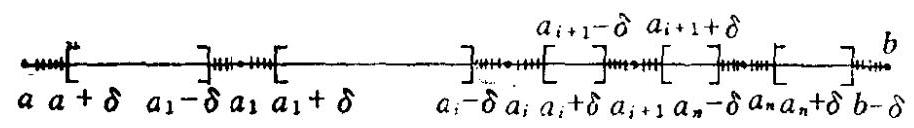
\includegraphics[max width=0.8\textwidth]{images/bo_d25ksc77aajc738obdgg_215_353_576_914_128_0.jpg}
\end{center}
\hspace*{3em} 

图 5-4

在每一个闭区间 $\left\lbrack  {{a}_{i} + \delta ,{a}_{i + 1} - \delta }\right\rbrack$ 上, $f$ 是连续的,于是 $f$ 在 $\left\lbrack  {{a}_{i} + \delta ,{a}_{i + 1} - \delta }\right\rbrack$ 上可积,从而存在阶梯函数 ${\varphi }_{i},{\psi }_{i} : \left\lbrack  {{a}_{i} + \delta }\right.$ , $\left. {{a}_{i + 1} - \delta }\right\rbrack   \rightarrow  \mathbf{R}$ ,使得
\begin{align*}
	&{\varphi }_{i}\left( x\right)  \leq  f\left( x\right)  \leq  {\psi }_{i}\left( x\right) ,\;\forall x \in  \left\lbrack  {{a}_{i} + \delta ,{a}_{i + 1} - \delta }\right\rbrack\\
	&\left( {i = 0,1,\cdots ,n}\right) \text{ , }\\
	&{\int }_{{a}_{i} + \delta }^{{a}_{i + 1} - \delta }\left( {{\psi }_{i} - {\varphi }_{i}}\right) \left( x\right) {dx} < \varepsilon \;\left( {i = 0,1,\cdots ,n}\right) .
\end{align*}

另一方面,函数 $f$ 在 $\left\lbrack  {a,b}\right\rbrack$ 上显然有界,故存在 $m,M \in  \mathbf{R}$ 使得
$$m \leq  f\left( x\right)  \leq  M,\;\forall x \in  \left\lbrack  {a,b}\right\rbrack  .$$

现在我们定义阶梯函数 $\varphi ,\psi  : \left\lbrack  {a,b}\right\rbrack   \rightarrow  \mathbf{R}$ 如下:
$$\varphi \left( x\right)  = \left\{  \begin{matrix} m & \left( {\text{ 若 }x \in  \left\lbrack  {\left\lbrack  {a,a + \delta \lbrack  \cup  \rbrack }\right\rbrack  b - \delta ,\;M}\right\rbrack  }\right) \\   & \left. {b\rbrack \bigcup \mathop{\bigcup }\limits_{{i = 1}}^{n}\left\lbrack  {{a}_{i} - \delta ,\;{a}_{i} + \delta \lbrack }\right\rbrack  }\right) \\  {\varphi }_{i}\left( x\right) & \left( {\text{ 若 }x \in  \left\lbrack  {{a}_{i} + \delta ,\;{a}_{i + 1} - \delta }\right\rbrack  \;{\psi }_{i}\left( x\right) }\right) \\  f\left( {{a}_{i} - \delta }\right) & \left( {\text{ 若 }x = {a}_{i} - \delta ,\;{\delta }_{i}}\right) \\   & \left( {f\left( {{a}_{i} + \delta }\right) ,\;{a}_{i} + \delta ,\;{a}_{i} + \delta }\right) \\  f\left( {{a}_{i} + \delta }\right) ,\;{\psi }_{i}\left( x\right) & \left( {\text{ 若 }x = {a}_{i} + \delta ,\;{\psi }_{i}\left( x\right)  + \delta }\right)  \end{matrix}\right\}   = \psi \left( x\right)$$

显然我们有
\begin{align*}
	&\varphi \left( x\right)  \leq  f\left( x\right)  \leq  \psi \left( x\right) ,\;\forall x \in  \left\lbrack  {a,b}\right\rbrack  ,\\
	&{\int }_{a}^{b}\left( {\psi  - \varphi }\right) \left( x\right) {dx} = {\int }_{a}^{a + \delta }\left( {\psi  - \varphi }\right) \left( x\right) {dx}\\
	&+ {\int }_{b - \delta }^{b}\left( {\psi  - \varphi }\right) \left( x\right) {dx} + \mathop{\sum }\limits_{{i = 1}}^{n}{\int }_{{a}_{i} - \delta }^{{a}_{i} + \delta }\left( {\psi  - \varphi }\right) \left( x\right) {dx}\\
	&+ \mathop{\sum }\limits_{{i = 0}}^{n}{\int }_{{a}_{i} + \delta }^{{a}_{i + 1} - \delta }\left( {\psi  - \varphi }\right) \left( x\right) {dx}\\
	&\leq  \left( {M - m}\right) \delta  + \left( {M - m}\right) \delta  + {2n}\left( {M - m}\right) \delta  + \left( {n + 1}\right) \overrightarrow{\varepsilon }\\
	&< \left\lbrack  {2\left( {n + 1}\right) \left( {M - m}\right)  + n + 1}\right\rbrack  \varepsilon .
\end{align*}

由此可知 $f$ 在 $\left\lbrack  {a,b}\right\rbrack$ 上可积.

定理 $5 \cdot  2 \cdot  4$ 任何一个单调函数 $f : \left\lbrack  {a,b}\right\rbrack   \rightarrow  \mathbf{R}$ 在 $\left\lbrack  {a,b}\right\rbrack$ 上是可积的.

证明 不失一般性,我们假设 $f$ 是单调上升函数.

若 $f\left( a\right)  = f\left( b\right)$ ,则 $f$ 为常值函数,它显然在 $\left\lbrack  {a,b}\right\rbrack$ 上可积. 下面我们设 $f\left( a\right)  < f\left( b\right)$ .

$\forall \varepsilon  > 0$ ,取 $n$ 充分大使得 $\frac{\left( {b - a}\right) \left( {f\left( b\right)  - f\left( a\right) }\right) }{n} < \varepsilon$ .

设 $\sigma  = \left( {a,a + \frac{b - a}{n},a + 2 \cdot  \frac{b - a}{n},\cdots ,a + \left( {n - 1}\right) \frac{b - a}{n}}\right.$ , $b)$ 是 $\left\lbrack  {a,b}\right\rbrack$ 的等步长 $\frac{b - a}{n}$ 的分割,于是我们有
\begin{align*}
	&f\left( {a}_{i}\right)  \leq  {m}_{i} = \mathop{\inf }\limits_{{x \in  \left\lbrack  {{a}_{i},{a}_{i + 1}}\right\rbrack  }}f\left( x\right)  \leq  {M}_{i} = \mathop{\sup }\limits_{{x \in  \left\lbrack  {{a}_{i},{a}_{i + 1}}\right\rbrack  }}f\left( x\right)  = f\left( {a}_{i + 1}\right)\\
	&\left( {i = 0,1,2,\cdots ,n - 1}\right) .
\end{align*}

现在定义阶梯函数 $f : \left\lbrack  {a,b}\right\rbrack   \rightarrow  \mathbf{R}$ 如下:
$$\varphi \left( x\right)  = \left\{  \begin{matrix} {m}_{i} & \left( {\text{ 若 }x \in  \rbrack {a}_{i},{a}_{i + 1}\lbrack ,}\right. & {M}_{i} \\   & \left. {i = 0,1,\cdots ,n}\right) & \\  f\left( {a}_{i}\right) & \left( {\text{ 若 }x = {a}_{i},i = 0,1,\cdots ,n}\right) & f\left( {a}_{i}\right)  \end{matrix}\right\}   = \psi \left( x\right) .$$

显然

\begin{itemize}
	\item $\infty$ .
\end{itemize}
\begin{align*}
	&\varphi \left( x\right)  \leq  f\left( x\right)  \leq  \psi \left( x\right) ,\;\forall x \in  \left\lbrack  {a,b}\right\rbrack  ,\\
	&{\int }_{a}^{b}\left( {\psi  - \varphi }\right) \left( x\right) {dx} = \mathop{\sum }\limits_{{i = 0}}^{{n - 1}}\left( {{M}_{i} - {m}_{i}}\right) \left( {{a}_{i + 1} - {a}_{i}}\right)\\
	&= \mathop{\sum }\limits_{{i = 0}}^{{n - 1}}\left\lbrack  {f\left( {a}_{i + 1}\right)  - f\left( {a}_{i}\right) }\right\rbrack  \frac{b - a}{n}\\
	&= \frac{b - a}{n}\left\lbrack  {f\left( b\right)  - f\left( a\right) }\right\rbrack\\
	&< \varepsilon \text{ . }
\end{align*}

因此 $f$ 在 $\left\lbrack  {a,b}\right\rbrack$ 上可积.

例 3 考虑如下定义的函数 $f : \left\lbrack  {0,1}\right\rbrack   \rightarrow  \mathbf{R}$ :

$f\left( 0\right)  = 0,f\left( x\right)  = \frac{1}{n},\;\forall x \in  \left\rbrack  {\frac{1}{n + 1},\frac{1}{n}}\right\rbrack  ,\;\left( {n \in  \mathbf{N}}\right) .$

\begin{center}
	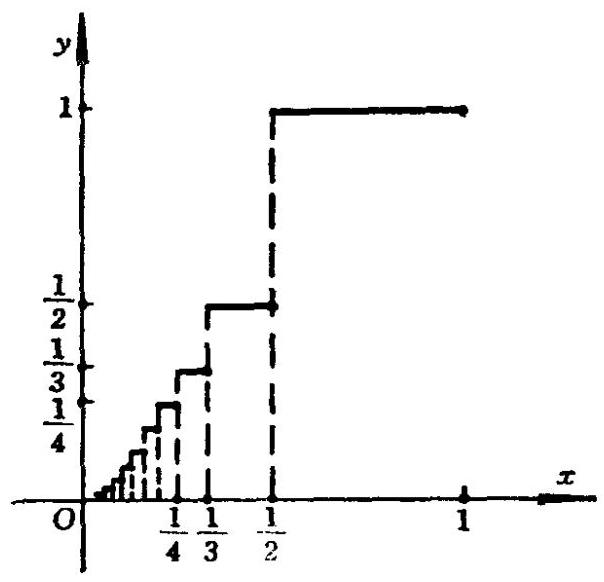
\includegraphics[max width=0.5\textwidth]{images/bo_d25ksc77aajc738obdgg_217_541_993_604_582_0.jpg}
\end{center}
\hspace*{3em} 

图 5-5

显然函数 $f$ 在 $\left\lbrack  {0,1}\right\rbrack$ 上是单调上升的,因此 $f$ 在 $\left\lbrack  {0,1}\right\rbrack$ 上可积.

下面我们介绍有界函数 $f : \left\lbrack  {a,b}\right\rbrack   \rightarrow  \mathrm{R}$ Riemann可积的第三个定理. 它是定理 $5 \cdot  2 \cdot  3$ 及其推论的推广.

为此先介绍零测度集的概念.

定义 设 $E \subset  \mathbf{R}$ 是任一集合,我们称 $E$ 是零测度集,如果 $\forall \varepsilon  > 0$ ,存在有限多个有界闭区间 $\left\lbrack  {{a}_{i},{b}_{i}}\right\rbrack  \left( {i = 1,2,\cdots ,m}\right)$ 使得
$$E \subset  \mathop{\bigcup }\limits_{{i = 1}}^{m}\left\lbrack  {{a}_{i},{b}_{i}}\right\rbrack  \text{ ,并且 }\mathop{\sum }\limits_{{i = 1}}^{m}\left( {{b}_{i} - {a}_{i}}\right)  < \bar{\varepsilon }\text{ . }$$

直接由此定义可推出下面几个简单结论:

1) $\mathbf{R}$ 的任何有限点集是零测度集.

2) 若 $\left\langle  {x}_{n}\right\rangle$ 是 $\mathbf{R}$ 的收敛点序列,则 $\left\{  {{x}_{n} \mid  n \in  \mathbf{N}}\right\}$ 是零测度集.

3) 若 $E$ 是零测度集,则 $E$ 的任一子集 $F$ 也是零测度集, $\bar{E}$ 也是零测度集.

4) 若 ${E}_{1},{E}_{2},\cdots ,{E}_{n}$ 是零测度集,则 $\mathop{\bigcup }\limits_{{i = 1}}^{n}{E}_{i}$ 也是零测度集.

定理 $5 \cdot  2 \cdot  5$ 若有界函数 $f : \left\lbrack  {a,b}\right\rbrack   \rightarrow  \mathbf{R}$ 的间断点集是零测度集,则 $f$ 在 $\left\lbrack  {a,b}\right\rbrack$ 上Riemann可积.

这个定理我们暂不在这里证明,因为它是第 19 章定理 ${19} \cdot  3 \cdot  6$  $n = 1$ 的情形.

但我们提醒读者注意: 定理 $5 \cdot  2 \cdot  5$ 的逆不成立,因此 $f$ 的间断点集是零测度集不是 $f$ Riemann 可积的充分必要条件. 下面就是一个反例.

例 4 考虑定义在 $\left\lbrack  {0,1}\right\rbrack$ 上的 Riemann 函数
$$x \mapsto  R\left( x\right)  = \left\{  \begin{array}{ll} 0, & \text{ 若 }x \in  \left\lbrack  {0,1}\right\rbrack   \cap  {\mathrm{Q}}^{c}; \\  1, & \text{ 若 }x = 0; \\  \frac{1}{p}, & \text{ 若 }x \in  \rbrack 0,1\rbrack  \cap  \mathrm{Q},x = \frac{q}{p},p,q\text{ 互质. } \end{array}\right.$$

我们知道此函数的间断点集 $E = \left\lbrack  {0,1}\right\rbrack   \cap  \mathbf{Q}$ ,但它不是零测度集,因为如果 $E$ 是零测度集,则 $\bar{E} = \left\lbrack  {0,1}\right\rbrack$ 也是零测度集,这显然矛盾.

下面证明此函数在 $\left\lbrack  {0,1}\right\rbrack$ 上 Riemann 可积,并且 ${\int }_{0}^{1}R\left( x\right) {dx}$  $= 0$ .

\begin{center}
	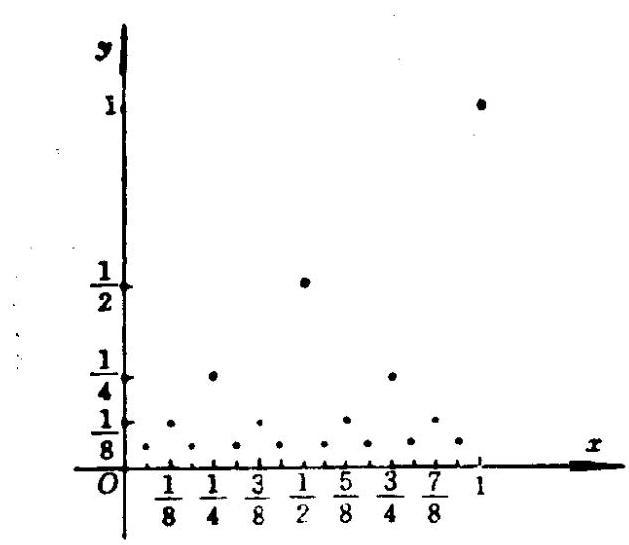
\includegraphics[max width=0.5\textwidth]{images/bo_d25ksc77aajc738obdgg_219_530_246_629_545_0.jpg}
\end{center}
\hspace*{3em} 

图 5-6

$\forall n \in  \mathbf{N}$ ,由 $\frac{1}{p} > \frac{1}{n}$ 知 $p < n$ . 故在 $\left\lbrack  {0,1}\right\rbrack$ 中满足 $\frac{1}{p} > \frac{1}{n}$ 的有理数只有有限个,记它们为 $0 = {x}_{0} < {x}_{1} < {x}_{2} < \cdots  < {x}_{m - 1} < {x}_{m} = 1$ . 定义阶梯函数 ${h}_{n},{k}_{n} : \left\lbrack  {0,1}\right\rbrack   \rightarrow  \mathbf{R}$ 为:
\begin{align*}
	&{h}_{n}\left( x\right)  = \left\{  \begin{array}{l} 0,\text{ 若 }x \in  \rbrack {x}_{i},{x}_{i + 1}\lbrack ,i = 0,1,\cdots ,m - 1, \\  R\left( x\right) \text{ 若 }x = {x}_{i},i = 0,1,\cdots ,m, \end{array}\right.\\
	&{k}_{n}\left( x\right)  = \frac{1}{n},\;\forall x \in  \left\lbrack  {0,1}\right\rbrack  .
\end{align*}

显然我们有
\begin{align*}
	&\left| {R\left( x\right)  - {h}_{n}\left( x\right) }\right|  \leq  {k}_{n}\left( x\right) ,\;\forall x \in  \left\lbrack  {0,1}\right\rbrack  ,\;\forall n \in  \mathbf{N},\\
	&\mathop{\lim }\limits_{{n \rightarrow   + \infty }}{\int }_{0}^{1}{k}_{n}\left( x\right) {dx} = \mathop{\lim }\limits_{{n \rightarrow   + \infty }}\frac{1}{n} = 0.
\end{align*}

因此由定理 $5 \cdot  2 \cdot  2$ 知, $R$ 在 $\left\lbrack  {0,1}\right\rbrack$ 上可积,并且
$${\int }_{0}^{1}R\left( x\right) {dx} = \mathop{\lim }\limits_{{n \rightarrow   + \infty }}{\int }_{0}^{1}{h}_{n}\left( x\right) {dx} = \mathop{\lim }\limits_{{n \rightarrow   + \infty }}\mathop{\sum }\limits_{{i = 0}}^{{m - 1}}{\int }_{{x}_{i}}^{{x}_{i + 1}}{h}_{n}\left( x\right) {dx} = 0.$$

现在我们要问: 是否存在使 $f$ Riemann 可积的充分必要条件呢? 回答是肯定的. 为此必须推广零测度集概念, 这一工作将在第 19 章进行.


\section*{5. Riemann可积函数的性质}

我们用 $\mathcal{B}\left\lbrack  {a,b}\right\rbrack$ 表示由定义在 $\left\lbrack  {a,b}\right\rbrack$ 上Riemann可积函数组成的集合,它是非空的,因 $\mathcal{E}\left\lbrack  {a,b}\right\rbrack   \subset  \mathcal{R}\left\lbrack  {a,b}\right\rbrack$ .

定理 $5 \cdot  2 \cdot  6$ 设 $f,g \in  \mathcal{R}\left\lbrack  {a,b}\right\rbrack  ,a,\beta  \in  \mathbf{R}$ ,则

1) ${\alpha f} + {\beta g} \in  \mathcal{P}\left\lbrack  {a,b}\right\rbrack$ ,且
$${\int }_{a}^{b}\left( {{af} + {\beta g}}\right) \left( x\right) {dx} = \alpha {\int }_{a}^{b}f\left( x\right) {dx} + \beta {\int }_{a}^{b}g\left( x\right) {dx}。$$

2) 若 $f \geq  0$ ,则 ${\int }_{a}^{b}f\left( x\right) {dx} \geq  0$ .

3) 若 $f \geq  g$ ,则 ${\int }_{a}^{b}f\left( x\right) {dx} \geq  {\int }_{a}^{b}g\left( x\right) {dx}$ .

4) $\left| f\right|  \in  \mathcal{R}\left\lbrack  {a,b}\right\rbrack$ ,且 $\left| {{\int }_{a}^{b}f\left( x\right) {dx}}\right|  \leq  {\int }_{a}^{b}\left| {f\left( x\right) }\right| {dx}$ .

证明 1 )因为 $f,g \in  \mathcal{R}\left\lbrack  {a,b}\right\rbrack$ ,所以存在两个阶梯函数族 ${\left\{  {h}_{n},{k}_{n}\right\}  }_{n \in  \mathbf{N}},{\left\{  {h}_{n},{k}_{n}\right\}  }_{n \in  \mathbf{N}}$ 使得
\begin{align*}
	&\left| {f\left( x\right)  - {h}_{n}\left( x\right) }\right|  \leq  {k}_{n}\left( x\right) ,\;\forall x \in  \left\lbrack  {a,b}\right\rbrack  ,\;\forall n \in  \mathbf{N},\\
	&\mathop{\lim }\limits_{{n \rightarrow   + \infty }}{\int }_{a}^{b}{k}_{n}\left( x\right) {dx} = 0,\\
	&\left| {g\left( x\right)  - {\widetilde{h}}_{n}\left( x\right) }\right|  \leq  {\widetilde{k}}_{n}\left( x\right) ,\;\forall x \in  \left\lbrack  {a,b}\right\rbrack  ,\;\forall n \in  \mathbf{N},\\
	&\mathop{\lim }\limits_{{n \rightarrow   + \infty }}{\int }_{a}^{b}{\widetilde{k}}_{n}\left( x\right) {dx} = 0,\\
	&{\int }_{a}^{b}f\left( x\right) {dx} = \mathop{\lim }\limits_{{n \rightarrow   + \infty }}{\int }_{a}^{b}{h}_{n}\left( x\right) {dx},\\
	&{\int }_{a}^{b}g\left( x\right) {dx} = \mathop{\lim }\limits_{{n \rightarrow   + \infty }}{\int }_{a}^{b}{\widetilde{h}}_{n}\left( x\right) {dx}.
\end{align*}

于是 $\alpha {h}_{n} + \beta {\widetilde{h}}_{n},\alpha {k}_{n} + \beta {\widetilde{k}}_{n} \in  \mathcal{E}\left\lbrack  {a,b}\right\rbrack  ,\forall n \in  \mathbf{N}$ ,并且
\begin{align*}
	&\left| {\left\lbrack  {{\alpha f} + {\beta g}}\right\rbrack  \left( x\right)  - \left\lbrack  {\alpha {h}_{n} + \beta {\widetilde{h}}_{n}}\right\rbrack  \left( x\right) }\right|  \leq  \left\lbrack  {\alpha {k}_{n} + \beta {\widetilde{k}}_{n}}\right\rbrack  \left( x\right) ,\\
	&\forall x \in  \left\lbrack  {a,b}\right\rbrack  ,\;\forall n \in  \mathbf{N}.\\
	&\mathop{\lim }\limits_{{n \rightarrow   + \infty }}{\int }_{a}^{b}\left\lbrack  {\alpha {k}_{n} + \beta {\widetilde{k}}_{n}}\right\rbrack  \left( x\right) {dx}\\
	&= \alpha \mathop{\lim }\limits_{{n \rightarrow   + \infty }}{\int }_{a}^{b}{k}_{n}\left( x\right) {dx} + \beta \mathop{\lim }\limits_{{n \rightarrow   + \infty }}{\int }_{a}^{b}{\widetilde{k}}_{n}\left( x\right) {dx} = 0.
\end{align*}

因此由定理 $5 \cdot  2 \cdot  2$ 知, ${\alpha f} + {\beta g} \in  \mathcal{R}\left\lbrack  {a,b}\right\rbrack$ ,并且
\begin{align*}
	&{\int }_{a}^{b}\left\lbrack  {{\alpha f} + {\beta g}}\right\rbrack  \left( x\right) {dx} = \mathop{\lim }\limits_{{n \rightarrow   + \infty }}{\int }_{a}^{b}\left\lbrack  {\alpha {h}_{n} + \beta {\widetilde{h}}_{n}}\right\rbrack  \left( x\right) {dx}\\
	&= \alpha \mathop{\lim }\limits_{{n \rightarrow   + \infty }}{\int }_{a}^{b}{h}_{n}\left( x\right) {dx} + \beta \mathop{\lim }\limits_{{n \rightarrow   + \infty }}{\int }_{a}^{b}{\widetilde{h}}_{n}\left( x\right) {dx}\\
	&= \alpha {\int }_{a}^{b}f\left( x\right) {dx} + \beta {\int }_{a}^{b}g\left( x\right) {dx}.
\end{align*}

2) 因为 $f \geq  0$ ,所以若令
$${h}_{n}^{ * }\left( x\right)  = \left\{  {\begin{array}{ll} {h}_{n}\left( x\right) , & \text{ 若 }{h}_{n}\left( x\right)  \geq  0, \\  0, & \text{ 若 }{h}_{n}\left( x\right)  < 0, \end{array}\;\forall x \in  \left\lbrack  {a,b}\right\rbrack  ,}\right.$$

则 ${h}_{n}^{ * } \in  \mathcal{E}\left\lbrack  {a,b}\right\rbrack$ 并且由 $\left| {f\left( x\right)  - {h}_{n}\left( x\right) }\right|  \leq  {k}_{n}\left( x\right)$ 得到
$${h}_{n}^{ * }\left( x\right)  - {k}_{n}\left( x\right)  \leq  f\left( x\right)  \leq  {h}_{n}^{ * }\left( x\right)  + {k}_{n}\left( x\right) ,\;\forall x \in  \left\lbrack  {a,b}\right\rbrack  .$$

因此
\begin{align*}
	&\left| {f\left( x\right)  - {h}_{n}^{ * }\left( x\right) }\right|  \leq  {k}_{n}\left( x\right) ,\;\forall x \in  \left\lbrack  {a,b}\right\rbrack  ,\;\forall n \in  \mathbf{N},\\
	&\mathop{\lim }\limits_{{n \rightarrow   + \infty }}{\int }_{a}^{b}{k}_{n}\left( x\right) {dx} = 0.
\end{align*}

此即表明阶梯函数族 ${\left\{  {h}_{n}^{ * },{k}_{n}\right\}  }_{n \in  \mathbb{N}}$ 适合函数 $f$ ,由 分定义,
$${\int }_{a}^{b}f\left( x\right) {dx} = \mathop{\lim }\limits_{{n \rightarrow   + \infty }}{\int }_{a}^{b}{h}_{n}^{ * }\left( x\right) {dx} \geq  0.$$

3) 若 $f \geq  g$ ,则 $f - g \geq  0$ ,从而由 1) 及 2) 知
$$0 \leq  {\int }_{a}^{b}\left( {f - g}\right) \left( x\right) {dx} = {\int }_{a}^{b}f\left( x\right) {dx} - {\int }_{a}^{b}g\left( x\right) {dx},$$

即 ${\int }_{a}^{b}f\left( x\right) {dx} \geq  {\int }_{a}^{b}g\left( x\right) {dx}$ .

4)由于
\begin{align*}
	&\left| \right| f\left( x\right) \left| -\right| {h}_{n}\left( x\right) \left| \right|  \leq  \left| {f\left( x\right)  - {h}_{n}\left( x\right) }\right|  \leq  {k}_{n}\left( x\right) ,\\
	&\forall x \in  \left\lbrack  {a,b}\right\rbrack  ,\;\forall n \in  \mathbf{N},\\
	&\mathop{\lim }\limits_{{n \rightarrow   + \infty }}{\int }_{a}^{b}{k}_{n}\left( x\right) {dx} = 0
\end{align*}

故阶梯函数族 ${\left\{  \left| {h}_{n}\right| ,{k}_{n}\right\}  }_{n \in  \mathbb{N}}$ 适合于函数 $\left| f\right|$ ,由定理 $5 \cdot  2 \cdot  2$ , $\left| f\right|  \in  \mathcal{R}\left\lbrack  {a,b}\right\rbrack$ ,并且由积分定义及定理 $5 \cdot  1 \cdot  1$ 知
\begin{align*}
	&{\int }_{a}^{b}\left| {f\left( x\right) }\right| {dx} = \mathop{\lim }\limits_{{n \rightarrow   + \infty }}{\int }_{a}^{b}\left| {{h}_{n}\left( x\right) }\right| {dx}\\
	&\geq  \mathop{\lim }\limits_{{n \rightarrow   + \infty }}\left| {{\int }_{a}^{b}{h}_{n}\left( x\right) {dx}}\right|  = \left| {{\int }_{a}^{b}f\left( x\right) {dx}}\right| .
\end{align*}

定理 $5 \cdot  2 \cdot  7$ 若 $f,g \in  \mathcal{R}\left\lbrack  {a,b}\right\rbrack$ ,则 ${fg} \in  \mathcal{R}\left\lbrack  {a,b}\right\rbrack$ .

证明 1) 首先假设 $f \geq  0,g \geq  0$ . 因 $f,g$ 有界,故存在 $M > 0$ ,使得
$$0 \leq  f\left( x\right)  \leq  M,0 \leq  g\left( x\right)  \leq  M,\;\forall x \in  \left\lbrack  {a,b}\right\rbrack  .$$

由于 $f,g \in  \mathcal{R}\left\lbrack  {a,b}\right\rbrack$ ,故由定义知, $\forall \varepsilon  > 0$ ,存在 $\varphi ,\psi ,\widetilde{\varphi }$ , $\psi  \in  \mathcal{E}\left\lbrack  {a,b}\right\rbrack$ ,使得
\begin{align*}
	&\varphi \left( x\right)  \leq  f\left( x\right)  \leq  \psi \left( x\right) ,\;\forall x \in  \left\lbrack  {a,b}\right\rbrack  ,\\
	&{\int }_{a}^{b}\left\lbrack  {\psi \left( x\right)  - \varphi \left( x\right) }\right\rbrack  {dx} < \frac{\varepsilon }{2M},\\
	&\widetilde{\varphi }\left( x\right)  \leq  g\left( x\right)  \leq  \widetilde{\psi }\left( x\right) ,\;\forall x \in  \left\lbrack  {a,b}\right\rbrack  ,\\
	&{\int }_{a}^{b}\left\lbrack  {\widetilde{\psi }\left( x\right)  - \widetilde{\varphi }\left( x\right) }\right\rbrack  {dx} < \frac{\varepsilon }{2M}.
\end{align*}

我们定义函数 $h,k,\widetilde{h},\widetilde{k} : \left\lbrack  {a,b}\right\rbrack   \rightarrow  \mathbf{R}$ 如下: $\forall x \in  \left\lbrack  {a,b}\right\rbrack$
\begin{align*}
	&h\left( x\right)  = \left\{  {\begin{array}{ll} \varphi \left( x\right) , & \text{ 若 }\varphi \left( x\right)  \geq  0, \\  0, & \text{ 若 }\varphi \left( x\right)  < 0; \end{array}\;k\left( x\right)  = \left\{  \begin{array}{ll} \psi \left( x\right) , & \text{ 若 }\psi \left( x\right)  \leq  M, \\  M, & \text{ 若 }\psi \left( x\right)  > M; \end{array}\right. }\right.\\
	&\widetilde{h}\left( x\right)  = \left\{  {\begin{array}{ll} \varphi \left( x\right) , & \text{ 若 }\varphi \left( x\right)  \geq  0, \\  0, & \text{ 若 }\varphi \left( x\right)  < 0; \end{array}\;\widetilde{k}\left( x\right)  = \left\{  \begin{array}{ll} \psi \left( x\right) , & \text{ 若 }\psi \left( x\right)  \leq  M, \\  M, & \text{ 若 }\widetilde{\psi }\left( x\right)  > M; \end{array}\right. }\right.
\end{align*}

则 $h,k,\widetilde{h},k \in  \mathcal{E}\left\lbrack  {a,b}\right\rbrack$ 并且.
\begin{align*}
	&\varphi \left( x\right)  \leq  h\left( x\right)  \leq  f\left( x\right)  \leq  k\left( x\right)  \leq  \psi \left( x\right) ,\;\forall x \in  \left\lbrack  {a,b}\right\rbrack  ,\\
	&{\int }_{a}^{b}\left\lbrack  {k\left( x\right)  - h\left( x\right) }\right\rbrack  {dx} \leq  {\int }_{a}^{b}\left\lbrack  {\psi \left( x\right)  - \varphi \left( x\right) }\right\rbrack  {dx} < \frac{\varepsilon }{2M},\\
	&\widetilde{\varphi }\left( x\right)  \leq  \widetilde{h}\left( x\right)  \leq  g\left( x\right)  \leq  \widetilde{k}\left( x\right)  \leq  \widetilde{\psi }\left( x\right) ,\;\forall x \in  \left\lbrack  {a,b}\right\rbrack  ,\\
	&{\int }_{a}^{b}\left\lbrack  {\widetilde{k}\left( x\right)  - \widetilde{h}\left( x\right) }\right\rbrack  {dx} \leq  {\int }_{a}^{b}\left\lbrack  {\widetilde{\psi }\left( x\right)  - \widetilde{\varphi }\left( x\right) }\right\rbrack  {dx} < \frac{\varepsilon }{2M}.
\end{align*}

由于 ${hh},{kh} \in  \mathcal{E}.\left\lbrack  {a,b}\right\rbrack$ ,并且 $f \geq  0,g \geq  0$ ,故我们有
\begin{align*}
	&\left( {hh}\right) \left( x\right)  \leq  \left( {fg}\right) \left( x\right)  \leq  \left( {kk}\right) \left( x\right) ,\;\forall x \in  \left\lbrack  {a,b}\right\rbrack  ,\\
	&{\int }_{a}^{b}\left\lbrack  {k\widetilde{k} - h\widetilde{h}}\right\rbrack  \left( x\right) {dx}\\
	&= {\int }_{a}^{b}\widetilde{k}\left( x\right) \left\lbrack  {k - h}\right\rbrack  \left( x\right) {dx} + {\int }_{a}^{b}h\left( x\right) \widetilde{k}\left\lbrack  {-\widetilde{h}}\right\rbrack  \left( x\right) {dx}\\
	&\leq  M{\int }_{a}^{b}\left\lbrack  {k\left( x\right)  - h\left( x\right) }\right\rbrack  {dx} + M{\int }_{a}^{b}\left\lbrack  {\widetilde{k}\left( x\right)  - \widetilde{h}\left( x\right) }\right\rbrack  {dx}\\
	&< M \cdot  \frac{\varepsilon }{2M} + M \cdot  \frac{\varepsilon }{2M} = \varepsilon .
\end{align*}

因此 ${fg} \in  \mathcal{R}\left\lbrack  {a,b}\right\rbrack$ .

2) 对一般的 $f,g$ ,令
$$m = \mathop{\inf }\limits_{{x \in  a}}f\left( x\right) ,\widetilde{m} = \mathop{\inf }\limits_{{x \in  a,b}}g\left( x\right) ,{f}^{ * } = f - m,{g}^{ * } = g - \widetilde{m},$$

则 ${f}^{ * } \geq  0,{g}^{ * } \geq  0$ ,并且 ${f}^{ * },{g}^{ * } \in  \mathcal{R}\left\lbrack  {a,b}\right\rbrack$ ,由 1 ) 所 证 ${f}^{ * }{g}^{ * } \in$  $\mathcal{R}\left\lbrack  {a,b}\right\rbrack$ ,于是由
$${f}^{ * }{g}^{ * } = \left( {f - m}\right) \left( {g - \widetilde{m}}\right)  = {fg} - \widetilde{m}f - {mg} + m\widetilde{m}$$

知, ${fg} \in  \mathcal{R}\left\lbrack  {a,b}\right\rbrack$ .

定理 $5 \cdot  2 \cdot  8$ 设 $f : \left\lbrack  {a,b}\right\rbrack   \rightarrow  \mathbf{R}$ 是任一函数, $c \in  \left\lbrack  {a,b}\right\rbrack$ . 那末 $f \in  \mathcal{R}\left\lbrack  {a,b}\right\rbrack$ 的充分必要条件是 ${\left. f\right| }_{\left( a,c\right) } \in  \mathcal{R}\left\lbrack  {a,c}\right\rbrack  ,{\left. f\right| }_{\left( c,b\right) } \in$  $\mathcal{R}\left\lbrack  {c,b}\right\rbrack$ ①. 并且这时
$${\int }_{a}^{b}f\left( x\right) {dx} = {\int }_{a}^{c}f\left( x\right) {dx} + {\int }_{c}^{b}f\left( x\right) {dx}.$$

\footnote{
	
	① 像对阶梯函数一样,我们约定: 若 $a = b$ ,则 $f : \left\lbrack  {a,b}\right\rbrack   \rightarrow  \mathbf{R}$ 是可积的,并且 ${\int }_{a}^{a}f\left( x\right) {dx} = 0.$
	
}

证明 1) 必要性 设 $f \in  \mathcal{B}\left\lbrack  {a,b}\right\rbrack$ . 若 $c = a$ 或 $c = b$ ,则由我们的约定知,定理显然成立. 因此我们设 $c \in  \rbrack a,b\lbrack$ . 由定理 $5 \cdot  2 \cdot  2$ 知,存在阶梯函数族 ${\left\{  {h}_{n},{k}_{n}\right\}  }_{n \in  \mathbf{N}}$ ,使得
\begin{align*}
	&\left| {f\left( x\right)  - {h}_{n}\left( x\right) }\right|  \leq  {k}_{n}\left( x\right) ,\;\forall x \in  \left\lbrack  {a,b}\right\rbrack  ,\;\forall n \in  \mathbf{N},\\
	&\mathop{\lim }\limits_{{n \rightarrow   + \infty }}{\int }_{a}^{b}{k}_{n}\left( x\right) {dx} = 0,\\
	&{\int }_{a}^{b}f\left( x\right) {dx} = \mathop{\lim }\limits_{{n \rightarrow   - \infty }}{\int }_{a}^{b}{h}_{n}\left( x\right) {dx}.
\end{align*}

现在我们令
$${\widetilde{h}}_{n} = {\left. {h}_{n}\right| }_{\left\lbrack  a,c\right\rbrack  },{\widetilde{k}}_{n} = {\left. {k}_{n}\right| }_{\left\lbrack  a,c\right. };{h}_{n}^{ * } = {\left. {h}_{n}\right| }_{\left\lbrack  c,b\right\rbrack  },{k}_{n}^{ * } = {\left. {k}_{n}\right| }_{\left\lbrack  c,b\right. }.$$

$\left( {n \in  \mathbf{N}}\right)$

则 ${\widetilde{h}}_{n},{\widetilde{k}}_{n} \in  \mathcal{E}\left\lbrack  {a,c}\right\rbrack  ,{h}_{n}^{ * },{k}_{n}^{ * } \in  \mathcal{E}\left\lbrack  {c,b}\right\rbrack  \;\left( {\forall n \in  \mathbf{N}}\right)$ ,并且
\begin{align*}
	&{\left| f\right| }_{\left\lbrack  a,c\right\rbrack  }\left( x\right)  - {\widetilde{h}}_{n}\left( x\right)  \mid   \leq  {\widetilde{k}}_{n}\left( x\right) ,\;\forall x \in  \left\lbrack  {a,c}\right\rbrack  ,\;\forall n \in  \mathbf{N},\\
	&{\int }_{a}^{c}{\widetilde{k}}_{n}\left( x\right) {dx} \leq  {\int }_{a}^{b}{k}_{n}\left( x\right) {dx},\\
	&{\left| f\right| }_{\left( c,b\right) }\left( x\right)  - {h}_{n}^{ * }\left( x\right)  \mid   \leq  {k}_{n}^{ * }\left( x\right) ,\;\forall x \in  \left\lbrack  {c,b}\right\rbrack  ,\;\forall n \in  \mathbf{N},\\
	&{\int }_{c}^{b}{k}_{n}^{ * }\left( x\right) {dx} \leq  {\int }_{a}^{b}{k}_{n}\left( x\right) {dx}.
\end{align*}

因此 $\mathop{\lim }\limits_{{n \rightarrow   + \infty }}{\int }_{a}^{o}\widetilde{k}\left( x\right) {dx} = 0,\;\mathop{\lim }\limits_{{n \rightarrow   + \infty }}{\int }_{c}^{b}{k}_{n}^{ * }\left( x\right) {dx} = 0$ ,

从而 ${\left. f\right| }_{\left\lbrack  a,c\right\rbrack  } \in  \mathcal{R}\left\lbrack  {a,c}\right\rbrack  ,{\left. f\right| }_{\left\lbrack  c,b\right\rbrack  } \in  \mathcal{R}\left\lbrack  {c,b}\right\rbrack$ ,并且
\begin{align*}
	&{\int }_{a}^{c}f\left( x\right) {dx} \triangleq  {\int }_{a}^{c}{\left. f\right| }_{\left\lbrack  a,c\right\rbrack  }\left( x\right) {dx} = \mathop{\lim }\limits_{{n \rightarrow   + \infty }}{\int }_{a}^{c}{\widetilde{h}}_{n}\left( x\right) {dx},\\
	&{\int }_{c}^{b}f\left( x\right) {dx} \triangleq  {\int }_{c}^{b}{\left. f\right| }_{\left\lbrack  c,b\right\rbrack  }\left( x\right) {dx} = \mathop{\lim }\limits_{{n \rightarrow   + \infty }}{\int }_{c}^{b}{h}_{n}^{ * }\left( x\right) {dx}.
\end{align*}

由于对阶梯函数 ${h}_{n} \in  \mathcal{E}\left\lbrack  {a,b}\right\rbrack$ ,我们有
$${\int }_{a}^{b}{h}_{n}\left( x\right) {dx} = {\int }_{a}^{c}{\widetilde{h}}_{n}\left( x\right) {dx} + {\int }_{c}^{b}{h}_{n}^{ * }\left( x\right) {dx}.$$

两边令 $n \rightarrow   + \infty$ 取极限得到
$${\int }_{a}^{b}f\left( x\right) {dx} = {\int }_{a}^{c}f\left( x\right) {dx} + {\int }_{c}^{b}f\left( x\right) {dx}.$$

2) 充分性 设 ${\left. f\right| }_{a,c)} \in  \mathcal{R}\left\lbrack  {a,c}\right\rbrack  ,{\left. f\right| }_{\left( c,b\right) } \in  \mathcal{R}\left\lbrack  {c,b}\right\rbrack$ . 不妨设 $c \in  \rbrack a,b\lbrack$ . 于是 $\forall \varepsilon  > 0$ ,存在 ${\varphi }_{1},{\psi }_{1} \in  \mathcal{E}\left\lbrack  {a,c}\right\rbrack$ 及, ${\varphi }_{2}$ , ${\psi }_{2} \in  \mathcal{E}\left\lbrack  {c,b}\right\rbrack$ 使得
\begin{align*}
	&{\varphi }_{1}\left( x\right)  \leq  {\left. f\right| }_{a,c}\;\left( x\right)  \leq  {\psi }_{1}\left( x\right) ,\;\forall x \in  \left\lbrack  {a,c}\right\rbrack  ,\\
	&{\int }_{a}^{c}\left\lbrack  {{\psi }_{1}\left( x\right)  - {\varphi }_{1}\left( x\right) }\right\rbrack  {dx} < \varepsilon /2,\\
	&{\varphi }_{2}\left( x\right)  \leq  {\left. f\right| }_{{ic},b}\left( x\right)  \leq  {\psi }_{2}\left( x\right) ,\;\forall x \in  \left\lbrack  {c,b}\right\rbrack  ,\\
	&{\int }_{c}^{b}\left\lbrack  {{\psi }_{2}\left( x\right)  - {\varphi }_{2}\left( x\right) }\right\rbrack  {dx} < \varepsilon /2.
\end{align*}

定义函数 $\varphi ,\psi  : \left\lbrack  {a,b}\right\rbrack   \rightarrow  \mathbf{R}$ 如下:
$$\varphi \left( x\right)  = \left\{  \begin{array}{lll} {\varphi }_{1}\left( x\right) & \text{ (若 }x \in  \left\lbrack  {a,c\left\lbrack  \right\rbrack  }\right\rbrack  & {\psi }_{1}\left( x\right) \\  f\left( c\right) & \text{ (若 }x = c) & f\left( c\right) \\  {\varphi }_{2}\left( x\right) & \text{ (若 }x \in  \rbrack c,b\rbrack ) & {\psi }_{2}\left( x\right)  \end{array}\right\}   = \psi \left( x\right)$$

则 $\varphi ,\psi  \in  \mathcal{E}\left\lbrack  {a,b}\right\rbrack$ ,并且
\begin{align*}
	&\varphi \left( x\right)  \leq  f\left( x\right)  \leq  \psi \left( x\right) ,\;\forall x \in  \left\lbrack  {a,b}\right\rbrack  ,\\
	&{\int }_{a}^{b}\left\lbrack  {\psi \left( x\right)  - \varphi \left( x\right) }\right\rbrack  {dx}\\
	&= {\int }_{a}^{c}\left\lbrack  {{\psi }_{1}\left( x\right)  - {\varphi }_{1}\left( x\right) }\right\rbrack  {dx} + {\int }_{c}^{b}\left\lbrack  {{\psi }_{2}\left( x\right)  - {\varphi }_{2}\left( x\right) }\right\rbrack  {dx} < \bar{\varepsilon }.
\end{align*}

因此 $f \in  \mathcal{R}\left\lbrack  {a,b}\right\rbrack$ .

现在我们作如下约定:

若 $f \in  \mathcal{R}\left\lbrack  {a,b}\right\rbrack$ ,则 $\forall c,d \in  \left\lbrack  {a,b}\right\rbrack$ 且 $c < d$ ,
$${\int }_{d}^{c}f\left( x\right)  \triangleq   - {\int }_{c}^{d}f\left( x\right) {dx}.$$

推论 设 $a,b,c \in  \mathbf{R}$ 并且
$$f : \left\lbrack  {\min \left( {a,b,c}\right) ,\max \left( {a,b,c}\right) }\right\rbrack   \rightarrow  \mathrm{R}$$

Riemann 可积. 则 $f$ 在由 $a,b,c$ 确定的每一个有限闭区间上 Riemann可积, 并且成立下述等式:
$${\int }_{a}^{b}f\left( x\right) {dx} = {\int }_{a}^{c}f\left( x\right) {dx} + {\int }_{c}^{b}f\left( x\right) {dx}.$$

证明 我们只对 $a < b < c$ 的情形进行证明. 其他情形的证明完全类似.

由定理 $5 \cdot  2 \cdot  8$ 知, ${\left. f\right| }_{\left( a,b\right. } \in  \mathcal{R}\left\lbrack  {a,b}\right\rbrack  ,{\left. f\right| }_{\left( b,c\right) } \in  \mathcal{R}\left\lbrack  {b,c}\right\rbrack$ , 并且
$${\int }_{a}^{c}f\left( x\right) {dx} = {\int }_{a}^{b}f\left( x\right) {dx} + {\int }_{b}^{c}f\left( x\right) {dx}.$$

由此得到
$${\int }_{a}^{b}f\left( x\right) {dx} = {\int }_{a}^{c}f\left( x\right) {dx} - {\int }_{b}^{c}f\left( x\right) {dx}.$$

根据我们的约定, $- {\int }_{b}^{c}f\left( x\right) {dx} = {\int }_{c}^{b}f\left( x\right) {dx}$ ,因此
$${\int }_{a}^{b}f\left( x\right) {dx} = {\int }_{a}^{c}f\left( x\right)  + {\int }_{c}^{b}f\left( x\right) {dx}.$$

例 5 设 $f : \left\lbrack  {a,b}\right\rbrack   \rightarrow  \mathbf{R}$ 是任一Riemann可积函数. ${a}_{0} \in  \left\lbrack  {a,b}\right\rbrack$ 是任一固定实数。根据定理 $5 \cdot  2 \cdot  8$ 及我们的约定, $\forall x \in  \left\lbrack  {a,b}\right\rbrack$ , ${\int }_{{a}_{0}}^{x}f\left( t\right) {dt}$ 有意义. 因此我们可以定义一个函数 $F : \left\lbrack  {a,b}\right\rbrack   \rightarrow  \mathbf{R}$ 如下:
$$\forall x \in  \left\lbrack  {a,b}\right\rbrack  ,F\left( x\right)  = {\int }_{{a}_{0}}^{x}f\left( t\right) {dt}.$$

函数 $F$ 称为 $f$ 的积分函数. 证明: $F$ 在 $\left\lbrack  {a,b}\right\rbrack$ 上一致连续.

事实上, $\forall {x}_{1},{x}_{2} \in  \left\lbrack  {a,b}\right\rbrack$ ,由上述推论我们有
\begin{align*}
	&\left| {F\left( {x}_{1}\right)  - F\left( {x}_{2}\right) }\right|  = \left| {{\int }_{{a}_{0}}^{{x}_{1}}f\left( t\right) {dt} - {\int }_{{a}_{0}}^{{x}_{2}}f\left( t\right) {dt}}\right|\\
	&= \left| {{\int }_{{x}_{2}}^{x1}f\left( t\right) {dt}}\right|\\
	&\leq  \left| {{x}_{1} - {x}_{2}}\right|  \cdot  \mathop{\sup }\limits_{{t \in  \left\lbrack  {a,b}\right\rbrack  }}\left| {f\left( t\right) }\right| .
\end{align*}

由于 $f$ 在 $\left\lbrack  {a,b}\right\rbrack$ 上有界,故 $M = \mathop{\sup }\limits_{a}\left| {f\left( t\right) }\right|  <  + \infty$ .

$\forall \varepsilon  > 0$ ,由 $\left( {1 + M}\right) \left| {{x}_{1} - {x}_{2}}\right|  < \varepsilon$ 得到 $\left| {{x}_{1} - {x}_{2}}\right|  < \frac{\varepsilon }{1 + M}$ . 若

令 $\delta  = \frac{\varepsilon }{1 + M}$ ,则
\begin{align*}
	&\forall {x}_{1},{x}_{2} \in  \left\lbrack  {a,b}\right\rbrack  \text{ 且 }\left| {{x}_{1} - {x}_{2}}\right|  < \delta  \Rightarrow  \left| {F\left( {x}_{1}\right)  - F\left( {x}_{2}\right) }\right|\\
	&< M\left| {{x}_{1} - {x}_{2}}\right|  < \varepsilon .
\end{align*}

因此 $F$ 在 $\left\lbrack  {a,b}\right\rbrack$ 上一致连续.

可积函数的积分函数,在我们后面的 $§4$ 中有重要应用.

定理 $5 \cdot  2 \cdot  9$ (第一积分中值公式) 设 $f,g \in  \mathcal{R}\left\lbrack  {a,b}\right\rbrack$ 并且 $g$ 在 $\left\lbrack  {a,b}\right\rbrack$ 上不变号. 令
$$m = \mathop{\inf }\limits_{{x \in   - a.b}}f\left( x\right) ,M = \mathop{\sup }\limits_{{x \in  \left\lbrack  {a,b}\right\rbrack  }}f\left( x\right) ,$$

则存在 $\lambda  \in  \left\lbrack  {m,M}\right\rbrack$ 使得
$${\int }_{a}^{b}f\left( x\right) g\left( x\right) {dx} = \lambda {\int }_{a}^{b}g\left( x\right) {dx}.$$

特别地,若 $f$ 在 $\left\lbrack  {a,b}\right\rbrack$ 上连续,则存在 $c \in  \left\lbrack  {a,b}\right\rbrack$ 使得
$${\int }_{a}^{b}f\left( x\right) g\left( x\right) {dx} = f\left( c\right) {\int }_{a}^{b}g\left( x\right) {dx}.$$

证明 首先由于 $f$ 在 $\left\lbrack  {a,b}\right\rbrack$ 上有界,故 $m,M \in  \mathbf{R}$ 并且
$$m \leq  f\left( x\right)  \leq  M,\;\forall x \in  \left\lbrack  {a,b}\right\rbrack  .$$

由于 $g$ 在 $\left\lbrack  {a,b}\right\rbrack$ 上不变号,不妨设 $g \geq  0$ ,将上述不等式乘以 $g$ 得到
$${mg}\left( x\right)  \leq  f\left( x\right) g\left( x\right)  \leq  {Mg}\left( x\right) ,\;\forall x \in  \left\lbrack  {a,b}\right\rbrack  .$$

由定理 $5 \cdot  2 \cdot  6$ 有
$$m{\int }_{a}^{b}g\left( x\right) {dx} \leq  {\int }_{a}^{b}f\left( x\right) g\left( x\right) {dx} \leq  M{\int }_{a}^{b}g\left( x\right) {dx}.$$

1) 若 ${\int }_{a}^{b}g\left( x\right) {dx} = 0$ ,则 ${\int }_{a}^{b}f\left( x\right) g\left( x\right) {dx} = 0$ ,从而任取 $\lambda  \in$  $\left\lbrack  {m,M}\right\rbrack$ ,成立
$${\int }_{a}^{b}f\left( x\right) g\left( x\right) {dx} = \lambda {\int }_{a}^{b}g\left( x\right) {dx}.$$

2) 若 ${\int }_{a}^{b}g\left( x\right) {dx} = 0$ ,则由 $g \geq  0$ 知 ${\int }_{a}^{b}g\left( x\right) {dx} > 0$ . 于是
$$m \leq  \frac{{\int }_{a}^{b}f\left( x\right) g\left( x\right) {dx}}{{\int }_{a}^{b}g\left( x\right) {dx}} \leq  M.$$
(*)

令 $\lambda  = {\int }_{a}^{b}f\left( x\right) g\left( x\right) {dx}/{\int }_{a}^{b}g\left( x\right) {dx}$ ,则 $\lambda  \in  \left\lbrack  {m,M}\right\rbrack$ ,并且
$${\int }_{a}^{b}f\left( x\right) g\left( x\right) {dx} = \lambda {\int }_{a}^{b}g\left( x\right) {dx}.$$

特别地,若 $f$ 在 $\left\lbrack  {a,b}\right\rbrack$ 上连续,则在 ${\int }_{a}^{b}g\left( x\right) {dx} = 0$ 时, $\forall c \in$  $\left\lbrack  {a,b}\right\rbrack$ 都有
$${\int }_{a}^{b}f\left( x\right) g\left( x\right) {dx} = f\left( c\right) {\int }_{a}^{b}g\left( x\right) {dx}.$$

在 ${\int }_{a}^{b}g\left( x\right) {dx} = 0$ 时,由连续函数的Weierstrass定理 及上述不等式 $\left( *\right)$ 知,存在 $c \in  \left\lbrack  {a,b}\right\rbrack$ 使得
$$f\left( c\right)  = {\int }_{a}^{b}f\left( x\right) g\left( x\right) {dx}/{\int }_{a}^{b}g\left( x\right) {dx},$$

因此
$${\int }_{a}^{b}f\left( x\right) g\left( x\right) {dx} = f\left( c\right) {\int }_{a}^{b}g\left( x\right) {dx}.$$

如果我们在上述定理中取 $g = 1$ ,则

1) 存在 $\lambda  \in  \left\lbrack  {m,M}\right\rbrack$ ,使得 ${\int }_{a}^{b}f\left( x\right) {dx} = \lambda \left( {b - a}\right)$ .

2) 特别地若 $f$ 连续,则存在 $c \in  \left\lbrack  {a,b}\right\rbrack$ 使得
$${\int }_{b}^{a}f\left( x\right) {dx} = f\left( c\right) \left( {b - a}\right) .$$

\section*{6. 积分的推广}

前面我们介绍的是一元实值函数的Riemann积分概念,下面我们要把它推广到一元复值函数上去.

设 $f : \left\lbrack  {a,b}\right\rbrack   \rightarrow  \mathrm{C}$ 是任一复值函数. $\forall x \in  \left\lbrack  {a,b}\right\rbrack$ ,令
$$f\left( x\right)  = {f}_{1}\left( x\right)  + i{f}_{2}\left( x\right) ,$$

于是我们得到与 $f$ 对应的两个一元实值函数 ${f}_{1},{f}_{2} : \left\lbrack  {a,b}\right\rbrack   \rightarrow  \mathrm{R}$ .

定义 我们称 $f$ 在 $\left\lbrack  {a,b}\right\rbrack$ 上可积,如果 ${f}_{1},{f}_{2}$ 在 $\left\lbrack  {a,b}\right\rbrack$ 上可积. 并且这时 $f$ 在 $\left\lbrack  {a,b}\right\rbrack$ 上的积分,记为 ${\int }_{a}^{b}f\left( x\right) {dx}$ ,定义为:
$${\int }_{a}^{b}f\left( x\right) {dx} = {\int }_{a}^{b}{f}_{1}\left( x\right) {dx} + i{\int }_{a}^{b}{f}_{2}\left( x\right) {dx}.$$

我们用 $\widetilde{\mathcal{R}}\left\lbrack  {a,b}\right\rbrack$ 表示所有定义在 $\left\lbrack  {a,b}\right\rbrack$ 上的可积复值函数的集合. $\mathcal{R}\left\lbrack  {a,b}\right\rbrack   = \varnothing$ ,因为 $\mathcal{R}\left\lbrack  {a,b}\right\rbrack   \subset  \mathcal{R}\left\lbrack  {a,b}\right\rbrack$ . 下面我们简单列出可积复值函数的两个基本性质, 读者自己补充其证明.

1) 若 $f,g \in  \widetilde{\mathcal{R}}\left\lbrack  {a,b}\right\rbrack  ,a,\beta  \in  \mathbf{C}$ ,则 ${af} + {\beta g} \in  \widetilde{\mathcal{R}}\left\lbrack  {a,b}\right\rbrack$ , 并且.
$${\int }_{a}^{b}\left( {{\alpha f} + {\beta g}}\right) \left( x\right) {dx} = \alpha {\int }_{a}^{b}f\left( x\right) {dx} + \beta {\int }_{a}^{b}g\left( x\right) {dx}.$$

2) 设 $c \in  \left\lbrack  {a,b}\right\rbrack$ ,则 $f \in  \widetilde{\mathcal{R}}\left\lbrack  {a,b}\right\rbrack   \Leftrightarrow  {\left. f\right| }_{\left\lbrack  a;o\right\rbrack  } \in$  $\widetilde{\mathcal{R}}\left\lbrack  {a,c}\right\rbrack  ,{\left. f\right| }_{\left\lbrack  c;b\right\rbrack  } \in  \widetilde{\mathcal{R}}\left\lbrack  {c,b}\right\rbrack$ ,且
$${\int }_{a}^{b}f\left( x\right) {dx} = {\int }_{a}^{c}f\left( x\right) {dx} + {\int }_{c}^{b}f\left( x\right) {dx}.$$

\section*{习 题}

1. 设 $f : \left\lbrack  {a,b}\right\rbrack   \rightarrow  \mathrm{R}$ 是任一函数. 证明下述两个结论等价:

1) $f$ 在 $\left\lbrack  {a,b}\right\rbrack$ 上Riemann可积.

2) $\forall \varepsilon  > 0$ ,存在 $\varphi ,\psi  \in  \mathcal{A}\left\lbrack  {a,b}\right\rbrack$ 使得
$$\varphi \left( x\right)  \leq  f\left( x\right)  \leq  \psi \left( x\right) ,\;\forall x \in  \left\lbrack  {a,b}\right\rbrack  ,{\int }_{a}^{b}\left\lbrack  {\psi \left( x\right)  - \varphi \left( x\right) }\right\rbrack  {dx} < \varepsilon .$$

2. 设 $f,g \in  \mathcal{B}\left\lbrack  {a,b}\right\rbrack  ,\forall x \in  \left\lbrack  {a,b}\right\rbrack$ 令

$m\left( x\right)  = \min \left( {f\left( x\right) ,g\left( x\right) }\right) ,M\left( x\right)  = \max \left( {f\left( x\right) ,g\left( x\right) }\right) ,$

证明: 函数 $m,M : \left\lbrack  {a,b}\right\rbrack   \rightarrow  R$ 在 $\left\lbrack  {a,b}\right\rbrack$ 上Riemann可积.

3. 设 $f \in  \mathcal{A}\left\lbrack  {a,b}\right\rbrack$ ,并且存在 $m > 0$ 使得 $\left| {f\left( x\right) }\right|  \geq  m\forall x \in  \left\lbrack  {a,b}\right\rbrack$ . 证 III: $\frac{1}{f} \in  \mathcal{R}\left\lbrack  {a,b}\right\rbrack$ .

4. 设 $f \in  \mathcal{R}\left\lbrack  {a,b}\right\rbrack$ ,并且 $f > 0$ . 证明 $\sqrt{f} \in  \mathcal{R}\left\lbrack  {a,b}\right\rbrack$ .

5. 设 $f : \left\lbrack  {a,b}\right\rbrack   \rightarrow  \mathbf{R}$ 是任一有界函数,考虑下列两对集合:
\begin{align*}
	&\Phi  = \{ \varphi  \in  \mathcal{E}\left\lbrack  {a,b}\right\rbrack   \mid  \varphi  \leq  f\} ,\;\Psi  = \{ \psi  \in  \mathcal{E}\left\lbrack  {a,b}\right\rbrack   \mid  f \leq  \Psi \} ,\\
	&H = \left\{  {{\int }_{a}^{b}\varphi \left( x\right) {dx} \mid  \varphi  \in  \Phi }\right\}  ,K = \left\{  {{\int }_{a}^{b}\psi \left( x\right) {dx} \mid  \psi  \in  \Psi }\right\}  .
\end{align*}

1) 证明: $\Phi  \neq  \varnothing ,\Psi  \neq  \varnothing$ .

2) 证明: $H$ 是上有界集, $K$ 是下有界集,并且 $\sup H \leq  \inf K$ . 我们记 $\iota \left( f\right)  = \sup H,s\left( f\right)  = \inf K$ ,并分别称 $i\left( f\right)$ 与 $s\left( f\right)$ 为 $f$ 在 $\left\lbrack  {a,b}\right\rbrack$ 上的下积分与上积分. 于是 $i\left( f\right)  \leq  s\left( f\right)$ .

3) 证明: $f$ 在 $\left\lbrack  {a,b}\right\rbrack$ 上Riemann可积的充分必要条件是 $i\left( f\right)  = s\left( f\right)$ , 并且这时 ${\int }_{a}^{b}f\left( x\right) {dx} = i\left( f\right)  = s\left( f\right)$ .

6. 设 $f : \left\lbrack  {a,b}\right\rbrack   \rightarrow  R$ 是任一有界函数. 我们称 $f$ 是正规的,如果下述性质成立:

$\forall x \in  \rbrack a,b\rbrack ,\mathop{\lim }\limits_{{y \rightarrow  {x}^{ - }}}f\left( y\right)  = f\left( {x}^{ - }\right)$ 存在, $\forall x \in  \left\lbrack  {a,b\left\lbrack  {,\mathop{\lim }\limits_{{y \rightarrow  {x}^{ + }}}f\left( y\right)  = }\right. }\right.$  $f\left( {x}^{ + }\right)$ 存在.

1) 证明: 若 $f$ 是单调函数,则 $f$ 是正规函数.

2 )证明:Riemann函数在 $\left\lbrack  {0,1}\right\rbrack$ 上是正规函数.

3) 设 ${f}^{\prime }\left\lbrack  {a,b}\right\rbrack   \rightarrow  R$ 是任一正规函数,

$a)$ 证明: $\forall \varepsilon  > 0$ ,存在 $\left\lbrack  {a,b}\right\rbrack$ 的一个分割 $\sigma  = \left( {{a}_{0},{a}_{1},\cdots ,{a}_{n}}\right)$ 使得

$\forall x,y \in  \rbrack {a}_{i},\;{a}_{n + 1}\lbrack ,i = 0,1,\cdots ,n - 1,\left| {f\left( x\right)  - f\left( y\right) }\right|  < \varepsilon .$

$b)$ 证明: $\forall \varepsilon  > 0$ ,存在 $h \in  \mathcal{E}\left\lbrack  {a,b}\right\rbrack$ ,使得
$$\left| {f\left( x\right)  - h\left( x\right) }\right|  < \varepsilon ,\;\forall x \in  \left\lbrack  {a,b}\right\rbrack  .$$

c) 由此推出 $f$ 在 $\left\lbrack  {a,b}\right\rbrack$ 上Riemann可积.

7. 设 $I \subset  R$ 是任一区间, $f : I \rightarrow  R$ 是任一函数. 我们称 $f$ 在 $I$ 上 局部 Riemann可积,若 $\forall \left\lbrack  {\alpha ,\beta }\right\rbrack   \subset  I,{\left. f\right| }_{\alpha ,\beta }$ 在 $\left\lbrack  {\alpha ,\beta }\right\rbrack$ 上是Riemann可积的.

1) 证明: 若函数 $f : \left\lbrack  {a,b}\right\rbrack   \rightarrow  R$ 有界并且在 $\rbrack a,b\lbrack$ 上局部Riemann 可积,则 $f$ 在 $\left\lbrack  {a,b}\right\rbrack$ 上Riemann可积.

2) 证明: 函数 $x \mid   \rightarrow  f\left( x\right)  = \left\{  \begin{matrix} \sin \frac{1}{x} & x \in  \rbrack 0,1\rbrack \\  0 & x = 0 \end{matrix}\right.$ 在 $\left\lbrack  {0,1}\right\rbrack$ 上不是正规的,但 $f$ 在 $\left\lbrack  {0,1}\right\rbrack$ 上Riemann可积.

8. 设 $f : \left\lbrack  {a,b}\right\rbrack   \rightarrow  \mathrm{R}$ 是任一有界函数. 并且 $f$ 的间断点集只有有限个聚点,证明 $f$ 在 $\left\lbrack  {a,b}\right\rbrack$ 上 $\mathrm{{Ri}} :$ mann 可积.

9. 设函数 $f : \left\lbrack  {a,b}\right\rbrack   \rightarrow  \mathbb{R}$ 在 $\left\lbrack  {a,b}\right\rbrack$ 上Riemann可积. 证明: $\forall e > 0$ , 存在连续函数 $g : \left\lbrack  {a,b}\right\rbrack   \rightarrow  \mathrm{R}$ 使得 ${\int }_{a}^{b}\left| {f\left( x\right)  - g\left( x\right) }\right| {dx} < \varepsilon$ .

10. 设 $f : \left\lbrack  {a,b}\right\rbrack   \rightarrow  \mathrm{R}$ 是任一函数. 证明:

1) 若 $f \geq  0$ ,并且 $f$ 在 $\left\lbrack  {a,b}\right\rbrack$ 上Riemann可积, $f$ 在连续点 $x$ 处满足 $f\left( x\right)  > 0$ . 则 ${\int }_{a}^{b}f\left( x\right) {dx} > 0$ .

2) 若 $f \geq  0$ , $f$ 在 $\left\lbrack  {a,b}\right\rbrack   \vdash  \operatorname{Riemann可积,并且}{\int }_{a}^{b}f\left( x\right) {dx} = 0$ ,则 $f$ 在连续点 $x$ 处满足 $f\left( x\right)  = 0$ .

11. 设 $f : \left\lbrack  {a,b}\right\rbrack   \rightarrow  \mathbf{R}$ 是任一Riemann可积函数. 证明: $\forall \left\lbrack  {\alpha ,\beta }\right\rbrack   =$  $\left\lbrack  {a,b}\right\rbrack$ .
$$\mathop{\lim }\limits_{{h \rightarrow  0}}{\int }_{\alpha }^{\beta }\left| {f\left( {x + h}\right)  - f\left( x\right) }\right| {dx} = 0.$$

12. 设 $f : \left\lbrack  {a,b}\right\rbrack   \rightarrow  R$ 在 $\left\lbrack  {a,b}\right\rbrack$ 上Riemann可积,证明: 存在 $\xi  \in  \left\lbrack  {a,b}\right\rbrack$ 使得 ${\int }_{a}^{\xi }f\left( x\right) {dx} = {\int }_{\xi }^{b}f\left( x\right) {dx}$ .

13. 我们用 $C\left( {\left\lbrack  {a,b}\right\rbrack  ,R}\right)$ 表示由所有定义在 $\left\lbrack  {a,b}\right\rbrack$ 上的连续函数组成的集合. $f \in  C\left( {\left\lbrack  {a,b}\right\rbrack  ,\mathrm{R}}\right)$ . 证明:

1) 若 $\forall g \in  C\left( {\left\lbrack  {a,b}\right\rbrack  ,R}\right) ,{\int }_{a}^{b}f\left( x\right) g\left( x\right) {dx} = 0$ ,则 $f = 0$ .

2) 若 $\forall g \in  C\left( {\left\lbrack  {a,b}\right\rbrack  ,\mathrm{R}}\right)$ 且 $g\left( a\right)  = g\left( b\right)  = 0,{\int }_{a}^{b}f\left( x\right) g\left( x\right) {dx} =$ 0,则 $f = 0$ .

14. 设 $f : \lbrack 0, + \infty \lbrack  \rightarrow  R$ 是任一连续函数,并且 $\mathop{\lim }\limits_{{x \rightarrow   + \infty }}f\left( x\right)  = A > 0$ 及 $\forall n \in  \mathbf{N},f\left( 0\right)  + f\left( 1\right)  + \cdots  + f\left( n\right)  \neq  0$ . 证明:
$$\mathop{\lim }\limits_{{n \rightarrow   + \infty }}\frac{{\int }_{0}^{\pi }f\left( x\right) {dx}}{f\left( 0\right)  + f\left( 1\right)  + \cdots  + f\left( n\right) } = 1.$$

15. 设 $f : \left\lbrack  {0 + \infty }\right\lbrack   \rightarrow  \left\lbrack  {0, + \infty }\right\lbrack$ 是任一严格单调上升的连续函数,并且 $f\left( {\lbrack 0, + \infty \lbrack }\right)  = \lbrack 0, + \infty \lbrack .$
$$\forall a > 0,b > 0,{\int }_{0}^{a}f\left( x\right) {dx} + {\int }_{0}^{b}{f}^{-1}\left( x\right) {dx} \geq  {ab}.$$

16. 设 $f,g \in  \mathcal{A}\left\lbrack  {a,b}\right\rbrack$ . 证明下述两个不等式:

1 ) Cauchy不等式
$${\left( {\int }_{a}^{b}f\left( x\right) g\left( x\right) dx\right) }^{2} \leq  {\int }_{a}^{b}{f}^{2}\left( x\right) {dx} \cdot  {\int }_{a}^{b}{g}^{2}\left( x\right) {dx}.$$

2 ) Minkowski不等式
\begin{align*}
	&{\left( {\int }_{a}^{b}{\left\lbrack  f\left( x\right)  + g\left( x\right) \right\rbrack  }^{2}dx\right) }^{\frac{1}{2}}\\
	&\leq  {\left( {\int }_{a}^{b}{f}^{2}\left( x\right) dx\right) }^{\frac{1}{2}} + {\left( {\int }_{a}^{b}{g}^{2}\left( x\right) dx\right) }^{\frac{1}{2}}.
\end{align*}

17. 设 $f,g : \left\lbrack  {a,b}\right\rbrack   \rightarrow  \mathbf{R}$ 是两个可积函数,令
$$M\left( g\right)  = \mathop{\sup }\limits_{{x \in  \left\lbrack  {a,b}\right\rbrack  }}f\left( x\right) ,\;m\left( g\right)  = \mathop{\inf }\limits_{{x \in  \left\lbrack  {a,b}\right\rbrack  }}g\left( x\right) ,\;m\left( g\right)  = \mathop{\inf }\limits_{{x \in  \left\lbrack  {a,b}\right\rbrack  }}g\left( x\right) ,$$

试利用Cauchy积分不等式证明:
\begin{align*}
	&\left| {\frac{1}{b - a}{\int }_{a}^{b}f\left( x\right) g\left( x\right) {dx} - \frac{1}{{\left( b - a\right) }^{2}}{\int }_{a}^{b}f\left( x\right) {dx} \cdot  {\int }_{a}^{b}g\left( x\right) {dx}}\right|\\
	&\leq  \frac{1}{4}\left( {M\left( f\right)  - m\left( f\right) }\right) \left( {M\left( g\right)  - m\left( g\right) }\right) .
\end{align*}

18. $\forall x \in  \left\lbrack  {0,1}\right\rbrack$ ,我们用 $0.{\varepsilon }_{1}{\varepsilon }_{2}{\varepsilon }_{3}\cdots \cdots$ 表示 $x$ 的十进制记法,定义函数 $f : \left\lbrack  {0,1}\right\rbrack   \rightarrow  \left\lbrack  {0,1}\right\rbrack$ 如下:
$$f\left( x\right)  = 0.{\varepsilon }_{2}{\varepsilon }_{1}{\varepsilon }_{3}\cdots ,\;\forall x = 0.{\varepsilon }_{1}{\varepsilon }_{2}{\varepsilon }_{3}\cdots$$

1) 研究函数 $f$ 在 $\left\lbrack  {0,1}\right\rbrack$ 上的连续性,证明 $f$ 的间断点都是第一类的, 并画出 $f$ 的图形.

2) 证明: $f$ 在 $\left\lbrack  {0,1}\right\rbrack$ 上可积,并且 ${\int }_{0}^{1}f\left( x\right) {dx} = \frac{1}{2}$ .

19. 设函数 $f : \left\lbrack  {a,b}\right\rbrack   \rightarrow  R$ 在 $\left\lbrack  {a,b}\right\rbrack$ 上可积. 证明:
$$\mathop{\lim }\limits_{{n \rightarrow   + \infty }}{\int }_{a}^{b}f\left( x\right) \left| {\sin {nx}}\right| {dx} = \frac{2}{\pi }{\int }_{a}^{b}f\left( x\right) {dx}.$$

(提示:先假设 $f$ 为在 $\left\lbrack  {\alpha ,\beta }\right\rbrack   \subset  \left\lbrack  {a,b}\right\rbrack$ 上取常值 $A$ 而在 $\left\lbrack  {a,b}\right\rbrack   - \left\lbrack  {\alpha ,\beta }\right\rbrack$ 上取 0 值的阶梯函数,然后利用 $f$ 的可积性,有阶梯函数 $h \in  g\left\lbrack  {a,b}\right\rbrack$ ,使得 ${\int }_{a}^{b}\left| {f\left( x\right)  - h\left( x\right) }\right| {dx} < {\varepsilon }_{0})$

20. 设 $f : \left\lbrack  {a,b}\right\rbrack   \rightarrow  R$ 可积, $g : \left\lbrack  {a,b}\right\rbrack   \rightarrow  R$ 连续 并且以 $T$ 为周期. 证明:
$$\mathop{\lim }\limits_{{n \rightarrow   + \infty }}{\int }_{a}^{b}f\left( x\right) g\left( {nx}\right) {dx} = \frac{1}{T}{\int }_{a}^{b}f\left( x\right) {dx} \cdot  {\int }_{0}^{T}g\left( x\right) {dx}.$$

\section{Riemann和}

在 $§2$ 里我们把Riemann可积函数的积分定义为一列阶梯函数积分的极限. 现在我们要把它表示成仅依赖于函数本身的另一种形式的极限. 为此引入下述定义.

定义 设 $f : \left\lbrack  {a,b}\right\rbrack   \rightarrow  \mathbf{R}$ 是任一函数. $\sigma  = \left( {{a}_{0},{a}_{1},\cdots ,{a}_{n}}\right)$ 是 $\left\lbrack  {a,b}\right\rbrack$ 的任一分割. $\xi  = \left\langle  {{\xi }_{0},{\xi }_{1},\cdots ,{\xi }_{n - 1}}\right\rangle$ 是一组实数,使得 ${\xi }_{i} \in  \left\lbrack  {{a}_{i},{a}_{i + 1}}\right\rbrack  \left( {i = 0,1,\cdots ,n - 1}\right) .$

1) $\left( {\sigma ,\xi }\right)$ 称为 $\left\lbrack  {a,b}\right\rbrack$ 的一个带点分割,并用 $\mathcal{B}$ 表示 $\left\lbrack  {a,b}\right\rbrack$ 的所有带点分割的集合.

2)实数
$$S\left( {f,\sigma ,\xi }\right)  = \mathop{\sum }\limits_{{i = 0}}^{{n - 1}}f\left( {\xi }_{i}\right) \left( {{a}_{i + 1} - {a}_{i}}\right)$$

称为函数 $f$ 关于 $\left( {\sigma ,\xi }\right)$ 的Riemann

3) 我们称实数 $A$ 是 $f$ 的Riemann和关于 $\mathcal{B}$ 的极限,如果下述性质成立:
\begin{align*}
	&\left( {\forall \varepsilon  > 0}\right) \left( {\exists \eta  > 0}\right) \left( {\forall \left( {\sigma ,\xi }\right)  \in  \mathcal{B},\delta \left( \sigma \right)  < \eta }\right)\\
	&\Rightarrow  \left| {S\left( {f,\sigma ,\xi }\right)  - A}\right|  < \varepsilon .
\end{align*}

这时, 我们记作
$$\mathop{\lim }\limits_{ \rightarrow  }S\left( {f,\sigma ,\xi }\right)  = A.$$

注意,上述 Riemann 和关于 $\mathcal{B}$ 的极限与函数极限的定义有点不一样,这里 $\left| {S\left( {f,\sigma ,\xi }\right)  - A}\right|  < \varepsilon$ 不仅要求 $\delta \left( \sigma \right)  < \eta$ ,而且 $\xi$ 在 $\sigma$ 确定后也可以任意选择. 因此 Riemann 和极限过程是比函数极限过程更复杂的一种极限过程.

定理 $5 \cdot  3 \cdot  1$ 设 $f : \left\lbrack  {a,b}\right\rbrack   \rightarrow  \mathbf{R}$ 是任一有界函数. 则下述两个结论等价:

1) $f$ 在 $\left\lbrack  {a,b}\right\rbrack$ 上Riemann可积.

2) 存在常数 $A$ 使得 $\mathop{\lim }\limits_{x}S\left( {f,\sigma ,\xi }\right)  = A$ . 因此若 $f \in  \mathcal{R}\left\lbrack  {a,b}\right\rbrack$ ,则
$${\int }_{a}^{b}f\left( x\right) {dx} = \mathop{\lim }\limits_{\mathcal{B}}S\left( {f,\sigma ,\xi }\right) .$$

证明 $1) \Rightarrow  2)$ . 设 $f \in  \mathcal{R}\left\lbrack  {a,b}\right\rbrack$ . 于是 $\forall \bar{\varepsilon } > 0,\exists h$ . $k \in  \mathcal{E}\left\lbrack  {a,b}\right\rbrack$ 使得
$$\left| {f\left( x\right)  - h\left( x\right) }\right|  \leq  k\left( x\right) ,\forall x \in  \left\lbrack  {a,b}\right\rbrack  ,{\int }_{a}^{b}k\left( x\right) {dx} < \varepsilon /4.$$

令 ${\sigma }_{0} = \left( {{b}_{0},{b}_{1},\cdots ,{b}_{m}}\right)$ 为同时适合于 $h\text{ 、 }k$ 的 $\left\lbrack  {a,b}\right\rbrack$ 的一个分割. 设 $\left| {f\left( x\right) }\right|  \leq  M,\forall x \in  \left\lbrack  {a,b}\right\rbrack$ .

取 $\eta  = \min \left( {\frac{1}{3}\delta \left( {\sigma }_{0}\right) ,\frac{\varepsilon }{{16}\left( {M + 1}\right) \left( {m + 1}\right) }}\right)$ ,则 $\eta  > 0$ .

对 ${\sigma }_{0}$ 的每一个分点 ${b}_{j}$ ,用闭区间 $\left\lbrack  {{b}_{j} - \eta ,{b}_{j} + \eta }\right\rbrack$ 把 ${b}_{j}$ 包围起来.

\begin{center}
	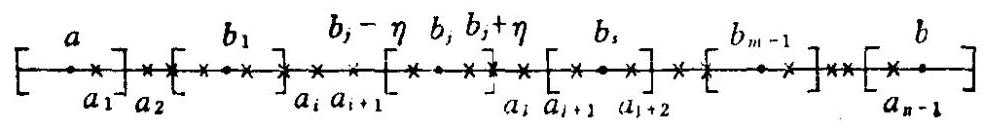
\includegraphics[max width=0.8\textwidth]{images/bo_d25ksc77aajc738obdgg_234_220_1513_987_129_0.jpg}
\end{center}
\hspace*{3em} 

图 5-7

现在设 $\left( {\sigma ,\xi }\right)  \in  \mathcal{B}$ ,并且 $\delta \left( \sigma \right)  < \eta$ . 令
$$\sigma  = \left( {{a}_{0},{a}_{1},\cdots ,{a}_{n}}\right) ,\xi  = \left\langle  {{\xi }_{0},{\xi }_{1},\cdots ,{\xi }_{n - 1}}\right\rangle  .$$

我们定义下面两个集合:
\begin{align*}
	&I = \{ i \in  \{ 0,1,\cdots ,n - 1\}  \mid  \forall j \in  \{ 0,1,\cdots ,m\} ,\\
	&\left\lbrack  {{a}_{i},{a}_{i + 1}}\right\rbrack   \cap  \left\lbrack  {{b}_{j} - \eta ,{b}_{j} + \eta }\right\rbrack   = \varnothing \} ,\\
	&J = \{ i \in  \{ 0,1,\cdots ,n - 1\}  \mid  \exists j \in  \{ 0,1,\cdots ,m\} ,\\
	&\left\lbrack  {{a}_{i},{a}_{i + 1}}\right\rbrack   \cap  \left\lbrack  {{b}_{j} - \eta ,{b}_{j} + \eta }\right\rbrack   \neq  \varnothing \} .
\end{align*}

显然 $I \cap  J = \varnothing ,I \cup  J = \{ 0,1,\cdots ,n - 1\}$ . 并且 $\forall i \in  J,\left\lbrack  {a}_{i}\right.$ , $\left. {a}_{i + 1}\right\rbrack   \subset  \rbrack {b}_{j} - \eta ,{b}_{j} + \eta \lbrack$ 或者 $\left\lbrack  {{a}_{i},{a}_{i + 1}}\right\rbrack$ 与 $\left\lbrack  {{b}_{j} - \eta ,{b}_{j} + \eta }\right\rbrack$ 有交点 ${b}_{j} - \eta$ 或 ${b}_{j} + \eta$ (如图 5-7 所示). 因此所有这种闭区间 $\left\lbrack  {{a}_{i},{a}_{i + 1}}\right\rbrack$ 的

长度之和 $\mathop{\sum }\limits_{{i \in  J}}\left( {{a}_{i + 1} - {a}_{i}}\right)$ 满足下述不等式:
\begin{align*}
	&\mathop{\sum }\limits_{{i \in  J}}\left( {{a}_{i + 1} - {a}_{i}}\right)  \leq  {2\eta }\left( {m + 1}\right)  + {2\delta }\left( \sigma \right) \left( {m + 1}\right)\\
	&< {4\eta }\left( {m + 1}\right)  < 4\left( {m + 1}\right)  \cdot  \frac{\varepsilon }{{16}\left( {M + 1}\right) \left( {m + 1}\right) }\\
	&= \frac{\varepsilon }{4\left( {M + 1}\right) }.
\end{align*}
(*)

下面我们来证明 $\left| {S\left( {f,\sigma ,\xi }\right)  - {\int }_{a}^{b}f\left( x\right) {dx}}\right|  < \varepsilon$ .

由于
\begin{align*}
	&\left| {S\left( {f,\sigma ,\xi }\right)  - {\int }_{a}^{b}f\left( x\right) {dx}}\right|\\
	&= \left| {\mathop{\sum }\limits_{{i = 0}}^{{n - 1}}f\left( {\xi }_{i}\right) \left( {{a}_{i + 1} - {a}_{i}}\right)  - \mathop{\sum }\limits_{{i = 0}}^{{n - 1}}{\int }_{{a}_{i}}^{{a}_{i + 1}}f\left( x\right) {dx}}\right|\\
	&= \left| {\mathop{\sum }\limits_{{i = 0}}^{{n - 1}}{\int }_{{a}_{i}}^{{a}_{i + 1}}f\left( {\xi }_{i}\right) {dx} - \mathop{\sum }\limits_{{i = 0}}^{{n - 1}}{\int }_{{a}_{i}}^{{a}_{i + 1}}f\left( x\right) {dx}}\right|\\
	&= \left| {\mathop{\sum }\limits_{{i = 0}}^{{n - 1}}{\int }_{{a}_{i}}^{{a}_{i + 1}}\left\lbrack  {f\left( {\xi }_{i}\right)  - f\left( x\right) }\right\rbrack  {dx}}\right|\\
	&\leq  \left| {\mathop{\sum }\limits_{{i \in  I}}{\int }_{{a}_{i}}^{{a}_{i + 1}}\left\lbrack  {f\left( {\xi }_{i}\right)  - f\left( x\right) }\right\rbrack  {dx}}\right|\\
	&+ \left| {\mathop{\sum }\limits_{{i \in  J}}{\int }_{{a}_{i}}^{{a}_{i + 1}}\left\lbrack  {f\left( {\xi }_{i}\right)  - f\left( x\right) }\right\rbrack  {dx}}\right| ,
\end{align*}

故我们分 $\left| \mathop{\sum }\limits_{{i \in  I}}\right|$ 与 $\left| \mathop{\sum }\limits_{{i \in  J}}\right|$ 两部分来估计.

i) $\left| {\mathop{\sum }\limits_{{i \in  I}}{\int }_{{a}_{i}}^{{a}_{i + 1}}\left\lbrack  {f\left( {\xi }_{i}\right)  - f\left( x\right) }\right\rbrack  {dx}}\right|$ 的估计:

我们注意到 $\forall i \in  I,\exists j \in  \{ 0,1,\cdots ,m - 1\}$ 使得 $\left\lbrack  {{a}_{i},{a}_{i + 1}}\right\rbrack$  $\subset  \rbrack {b}_{j},{b}_{j + 1}\left\lbrack  \right.$ . 于是由 $x,{\xi }_{i} \in  \left\lbrack  {{a}_{i},{a}_{i + 1}}\right\rbrack$ 知, $x,{\xi }_{i} \in  \rbrack {b}_{j},{b}_{j + 1}\lbrack$ . 因此
$$\forall x \in  \left\lbrack  {{a}_{i},{a}_{i + 1}}\right\rbrack  ,h\left( x\right)  = h\left( {\xi }_{i}\right) ,k\left( x\right)  = k\left( {\xi }_{i}\right) .$$

由于
\begin{align*}
	&\left| {f\left( {\xi }_{i}\right)  - h\left( {\xi }_{i}\right) }\right|  \leq  k\left( {\xi }_{i}\right) ,\left| {f\left( x\right)  - h\left( x\right) }\right|  \leq  k\left( x\right) ,\\
	&\forall x \in  \left\lbrack  {{a}_{i},{a}_{i + 1}}\right\rbrack  ,
\end{align*}

故
\begin{align*}
	&\left| {{\int }_{{a}_{i}}^{{a}_{i + 1}}\left\lbrack  {f\left( {\xi }_{i}\right)  - f\left( x\right) }\right\rbrack  {dx}}\right|\\
	&\leq  {\int }_{{a}_{i}}^{{a}_{i + 1}}\left| {f\left( {\xi }_{i}\right)  - h\left( {\xi }_{i}\right) }\right| {dx} + {\int }_{{a}_{i}}^{{a}_{i + 1}}\left| {h\left( {\xi }_{i}\right)  - f\left( x\right) }\right| {dx}\\
	&\leq  {\int }_{{a}_{i}}^{{a}_{i + 1}}k\left( {\xi }_{i}\right) {dx} + {\int }_{{a}_{i}}^{{a}_{i + 1}}k\left( x\right) {dx}\\
	&= 2{\int }_{{a}_{i}}^{{a}_{i} + 1}k\left( x\right) {dx}.
\end{align*}

由此得到
\begin{align*}
	&\left| {\mathop{\sum }\limits_{{i \in  I}}{\int }_{{a}_{i}}^{{a}_{i + 1}}\left\lbrack  {f\left( {\xi }_{i}\right)  - f\left( x\right) }\right\rbrack  {dx}}\right|\\
	&\leq  \mathop{\sum }\limits_{{i \in  I}}\left| {{\int }_{{a}_{i}}^{{a}_{i + 1}}\left\lbrack  {f\left( {\xi }_{i}\right)  - f\left( x\right) }\right\rbrack  {dx}}\right|\\
	&\leq  2\mathop{\sum }\limits_{{i \in  I}}{\int }_{{a}_{i}}^{{a}_{i + 1}}k\left( x\right) {dx}\\
	&\leq  2{\int }_{a}^{b}k\left( x\right) {dx} < 2 \cdot  \frac{\varepsilon }{4} = \frac{\varepsilon }{2}.
\end{align*}

ii) $\left| {\mathop{\sum }\limits_{{i \in  J}}{\int }_{{a}_{i}}^{{a}_{i + 1}}\left\lbrack  {f\left( {\xi }_{i}\right)  - f\left( x\right) }\right\rbrack  {dx}}\right|$ 的估计:

$\forall i \in  J$ ,我们有
\begin{align*}
	&\left| {{\int }_{{a}_{i}}^{{a}_{i + 1}}\left\lbrack  {f\left( {\xi }_{i}\right)  - f\left( x\right) }\right\rbrack  {dx}}\right|\\
	&\leq  {\int }_{{a}_{i}}^{{a}_{i + 1}}\left| {f\left( {\xi }_{i}\right)  - f\left( x\right) }\right| {dx} \leq  {2M}\left( {{a}_{i + 1} - {a}_{i}}\right) .
\end{align*}

从而由不等式 (*) 得到
\begin{align*}
	&\left| {\mathop{\sum }\limits_{{i \in  J}}{\int }_{{a}_{i}}^{{a}_{i + 1}}\left\lbrack  {f\left( {\xi }_{i}\right)  - f\left( x\right) }\right\rbrack  {dx}}\right|\\
	&\leq  \mathop{\sum }\limits_{{i \in  J}}\left| {{\int }_{{a}_{i}}^{{a}_{i + 1}}\left\lbrack  {f\left( {\xi }_{i}\right)  - f\left( x\right) }\right\rbrack  {dx}}\right|\\
	&\leq  \mathop{\sum }\limits_{{i \in  J}}{2M}\left( {{a}_{i + 1} - {a}_{i}}\right)\\
	&\leq  {2M} \cdot  \frac{\varepsilon }{4\left( {M + 1}\right) } < \frac{\varepsilon }{2}.
\end{align*}

现在由i) 和 ii) 的估计得到
\begin{align*}
	&\left| {S\left( {f,\sigma ,\xi }\right)  - {\int }_{a}^{b}f\left( x\right) {dx}}\right|\\
	&\leq  \left| {\mathop{\sum }\limits_{{i \in  I}}{\int }_{{a}_{i}}^{{a}_{i + 1}}\left\lbrack  {f\left( {\xi }_{i}\right)  - f\left( x\right) }\right\rbrack  {dx}}\right|\\
	&+ \left| {\mathop{\sum }\limits_{{i \in  J}}{\int }_{{a}_{i}}^{{a}_{i + 1}}\left\lbrack  {f\left( {\xi }_{i}\right)  - f\left( x\right) }\right\rbrack  {dx}}\right|\\
	&< \frac{\varepsilon }{2} + \frac{\varepsilon }{2} = \varepsilon .
\end{align*}

因此 $\mathop{\lim }\limits_{x}S\left( {f,\sigma ,\xi }\right)  = {\int }_{a}^{b}f\left( x\right) {dx}$ .

$2) \Rightarrow  1)$ 设存在常数 $A$ 使得 $\mathop{\lim }\limits_{x}S\left( {f,\sigma ,\xi }\right)  = A$ ,即
\begin{align*}
	&\left( {\forall \varepsilon  > 0}\right) \left( {\exists \eta  > 0}\right) \left( {\forall \left( {\sigma ,\xi }\right)  \in  \mathcal{B},\delta \left( \sigma \right)  < \eta }\right)\\
	&\Rightarrow  \left| {S\left( {f,\sigma ,\xi }\right)  - A}\right|  < \varepsilon .
\end{align*}

设 $\sigma  = \left( {{a}_{0},{a}_{1},\cdots ,{a}_{n}}\right)$ 是 $\left\lbrack  {a,b}\right\rbrack$ 的任一分割且 $\delta \left( \sigma \right)  < \eta$ . 令
$${m}_{i} = \mathop{\inf }\limits_{{x \in  \left\lbrack  {{a}_{i},{a}_{i + 1}}\right\rbrack  }}f\left( x\right) ,\;{M}_{i} = \mathop{\sup }\limits_{{x \in  \left\lbrack  {{a}_{i},{a}_{i + 1}}\right\rbrack  }}f\left( x\right) ,i = 0,1,\cdots ,n - 1.$$

构造函数 $\varphi ,\psi  : \left\lbrack  {a,b}\right\rbrack   \rightarrow  \mathbf{R}$ 如下:
$$\varphi \left( x\right)  = \left\{  \begin{matrix} {m}_{i} & \text{ (若 }x \in  \rbrack {a}_{i},{a}_{i + 1}\lbrack , & {M}_{i} \\   & i = 0,1,\cdots ,n - 1) & \\  f\left( {a}_{i}\right) & \text{ (若 }x = {a}_{i},i = 0,1,\cdots ,n) & f\left( {a}_{i}\right)  \end{matrix}\right\}   = \psi \left( x\right)$$

则 $\varphi ,\psi  \in  \mathcal{E}\left\lbrack  {a,b}\right\rbrack$ ,并且
$$\varphi \left( x\right)  \leq  f\left( x\right)  \leq  \psi \left( x\right) ,\;\forall x \in  \left\lbrack  {a,b}\right\rbrack  .$$

另一方面,利用确界特征性 ${\text{  }}^{r}$ . 存在 ${\xi }_{i}^{\prime },{\xi }_{i}^{\prime \prime } \in  \left\lbrack  {{a}_{i},{a}_{i + 1}}\right\rbrack$ 使得
\begin{align*}
	&{m}_{i} \leq  f\left( {\xi }_{i}^{\prime }\right)  < {m}_{i} + \frac{\varepsilon }{4\left( {b - a}\right) },\\
	&\left( {i = 0,1,\cdots ,n - 1}\right)\\
	&{M}_{i} - \frac{\varepsilon }{4\left( {b - a}\right) } < f\left( {\xi }_{i}^{\prime \prime }\right)  \leq  {M}_{i}.
\end{align*}

于是
\begin{align*}
	&\left| {f\left( {\xi }_{i}^{\prime }\right)  - {m}_{i}}\right|  < \frac{\bar{\varepsilon }}{4\left( {b - a}\right) },\left| {f\left( {\xi }_{i}^{\prime \prime }\right)  - {M}_{i}}\right|  < \frac{\bar{\varepsilon }}{4\left( {b - a}\right) }\\
	&\left( {i = 0,1,\cdots ,n - 1}\right) 。
\end{align*}

令 ${\xi }^{\prime } = \left\langle  {{\xi }_{0}^{\prime },{\xi }_{1}^{\prime },\cdots ,{\xi }_{n - 1}^{\prime }}\right\rangle  ,{\xi }^{\prime \prime } = \left\langle  {{\xi }_{0}^{\prime \prime },{\xi }_{1}^{\prime \prime },\cdots ,{\xi }_{n - 1}^{\prime \prime }}\right\rangle$ ,则我们有 $\left( {\sigma ,{\xi }^{\prime }}\right)  \in  \mathcal{B},\left( {\sigma ,{\xi }^{\prime \prime }}\right)  \in  \mathcal{B}$ 并且 $\delta \left( \sigma \right)  < \eta$ . 因此
$$\left| {S\left( {f,\sigma ,{\xi }^{\prime }}\right)  - A}\right|  < \frac{\varepsilon }{4},\;\left| {S\left( {f,\sigma ,{\xi }^{\prime \prime }}\right)  - A}\right|  < \frac{\varepsilon }{4}.$$

现在
\begin{align*}
	&\left| {S\left( {f,\sigma ,{\xi }^{\prime }}\right)  - {\int }_{a}^{b}\varphi \left( x\right) {dx}}\right|\\
	&= \left| {\mathop{\sum }\limits_{{i = 0}}^{{n - 1}}f\left( {\xi }_{i}^{\prime }\right) \left( {{a}_{i + 1} - {a}_{i}}\right)  - \mathop{\sum }\limits_{{i = 0}}^{{n - 1}}{m}_{i}\left( {{a}_{i + 1} - {a}_{i}}\right) }\right|\\
	&\leq  \mathop{\sum }\limits_{{i = 0}}^{{n - 1}}\left| {f\left( {\xi }_{i}^{\prime }\right)  - {m}_{i}}\right| \left( {{a}_{i + 1} - {a}_{i}}\right)\\
	&< \frac{\varepsilon }{4\left( {b - a}\right) }\left( {b - a}\right)  = \frac{\varepsilon }{4},\\
	&\left| {S\left( {f,\sigma ,{\xi }^{\prime \prime }}\right)  - {\int }_{a}^{b}\psi \left( x\right) {dx}}\right|\\
	&= \left| {\mathop{\sum }\limits_{{i = 0}}^{{n - 1}}f\left( {\xi }_{i}^{\prime \prime }\right) \left( {{a}_{i + 1} - {a}_{i}}\right)  - \mathop{\sum }\limits_{{i = 0}}^{{n - 1}}{M}_{i}\left( {{a}_{i + 1} - {a}_{i}}\right) }\right|\\
	&\leq  \mathop{\sum }\limits_{{i = 0}}^{{n - 1}}\left| {f\left( {\xi }_{i}^{\prime \prime }\right)  - {M}_{i}}\right| \left( {{a}_{i + 1} - {a}_{i}}\right)\\
	&< \frac{\varepsilon }{4\left( {b - a}\right) }\left( {b - a}\right)  = \frac{\varepsilon }{4}.
\end{align*}

因此最后我们得到
\begin{align*}
	&0 \leq  {\int }_{a}^{b}\left\lbrack  {\psi \left( x\right)  - \varphi \left( x\right) }\right\rbrack  {dx}\\
	&= \left| {{\int }_{a}^{b}\psi \left( x\right) {dx} - {\int }_{a}^{b}\varphi \left( x\right) {dx}}\right|\\
	&\leq  \left| {{\int }_{a}^{b}\psi \left( x\right) {dx} - S\left( {f,\sigma ,{\xi }^{\prime \prime }}\right) }\right|\\
	&+ \left| {S\left( {f,\sigma ,{\xi }^{\prime \prime }}\right)  - A}\right|  + \left| {A - S\left( {f,\sigma ,{\xi }^{\prime }}\right) }\right|\\
	&+ \left| {S\left( {f,\sigma ,{\xi }^{\prime }}\right)  - {\int }_{a}^{b}\varphi \left( x\right) {dx}}\right|\\
	&< \frac{\varepsilon }{4} + \frac{\ddot{\varepsilon }}{4} + \frac{\ddot{\varepsilon }}{4} + \frac{\dot{\varepsilon }}{4} = {\varepsilon }_{ \circ  }
\end{align*}

此即表明 $f$ 在 $\left\lbrack  {a,b}\right\rbrack$ 上 Riemann 可积. 并且这时 $A = {\int }_{a}^{b}f\left( x\right) {dx}$ .

推论 若 $f \in  \mathcal{R}\left\lbrack  {a,b}\right\rbrack$ ,则
\begin{align*}
	&\mathop{\lim }\limits_{{n \rightarrow   + \infty }}\mathop{\sum }\limits_{{i = 0}}^{{n - 1}}f\left( {a + i\frac{b - a}{n}}\right) \frac{b - a}{n} = {\int }_{a}^{b}f\left( x\right) {dx},\\
	&\mathop{\lim }\limits_{{n \rightarrow   + \infty }}\mathop{\sum }\limits_{{i = 1}}^{n}f\left( {a + i\frac{b - a}{n}}\right) \frac{b - a}{n} = {\int }_{a}^{b}f\left( x\right) {dx}.
\end{align*}

从这个推论来看,函数 $f : \left\lbrack  {a,b}\right\rbrack   \rightarrow  \mathbf{R}$ 的 Riemann 积分 ${\int }_{a}^{b}f\left( x\right) {dx}$ 的几何意义就十分明显.

将 $\left\lbrack  {a,b}\right\rbrack  n$ 等分,作出 $\frac{b - a}{n}$ 为底,以 $f\left( {a + i\frac{b - a}{n}}\right)$ 为 “高” 的に方形 ${S}_{i}$ ,则 ${S}_{i}$ 的 “面积” 为 $f\left( {a + i\frac{b - a}{n}}\right) \frac{b - a}{n}$ (这里 我们规定当 $f\left( {a + i\frac{b - a}{n}}\right)  \geq  0$ 时 ${S}_{i}$ 的 “面积” $\geq  0$ ,当 $f\left( {a + i\frac{b - a}{n}}\right)  < 0$ 时, ${S}_{i}$ 的 “面积” $< 0$ ),因此

$\mathop{\sum }\limits_{{i = 0}}^{{n - 1}}f\left( {a + i\frac{b - a}{n}}\right) \frac{b - a}{n} = {S}_{0},{S}_{1},\cdots ,{S}_{n - 1}$ 的 “面积” 之

和,
$$\mathop{\sum }\limits_{{i = 1}}^{n}f\left( {a + i\frac{b - a}{n}}\right) \frac{b - a}{n} = {S}_{1},{S}_{2},\cdots ,{S}_{n}\text{ 的 “面积” 之和. }$$

上述推论表明,当 $n \rightarrow   + \infty$ 时, ${S}_{0},{S}_{1},\cdots ,{S}_{n - 1}$ 的 “面积” 之和或 ${S}_{1},{S}_{2},\cdots ,{S}_{n}$ 的 “面积” 之和的极限 存 在,并且等于 $f$ 在 $\left\lbrack  {a,b}\right\rbrack$ 上的Riemann 积分 ${\int }_{a}^{b}f\left( x\right) {dx}$ ,因此 ${\int }_{a}^{b}f\left( x\right) {dx}$ 就 是由函数 $f$ 的图形 $\operatorname{Gr}\left( f\right)$ 、 $x$ 轴及直线 $x = a,x = b$ 所围平面区域的面积 (如图 5-8所示).

\begin{center}
	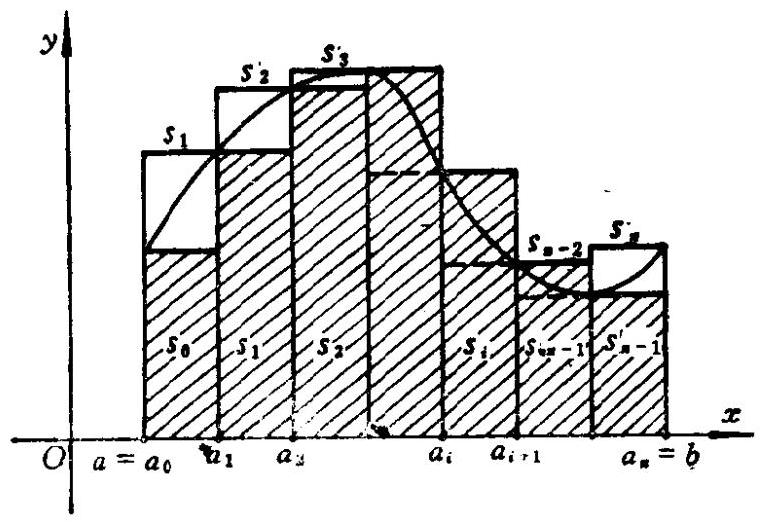
\includegraphics[max width=0.6\textwidth]{images/bo_d25ksc77aajc738obdgg_240_335_1447_760_522_0.jpg}
\end{center}
\hspace*{3em} 

图 5-8

例 1 计算 ${\int }_{0}^{1}{xdx}$ 与 ${\int }_{0}^{1}{x}^{2}{dx}$ 的值.

定义函数 $f,g : \left\lbrack  {0,1}\right\rbrack   \rightarrow  R$ 如下:
$$\forall x \in  \left\lbrack  {0,1}\right\rbrack  ,f\left( x\right)  = x,g\left( x\right)  = {x}^{2}.$$

则函数 $f,g$ 在 $\left\lbrack  {0,1}\right\rbrack$ 上连续,因而在 $\left\lbrack  {0,1}\right\rbrack$ 上Riemann可积. 根据上述推论有
\begin{align*}
	&{\int }_{0}^{1}{xdx} = \mathop{\lim }\limits_{{n \rightarrow   + \infty }}\mathop{\sum }\limits_{{i = 0}}^{{n - 1}}f\left( {0 + i\frac{1}{n}}\right)  \cdot  \frac{1}{n}\\
	&= \mathop{\lim }\limits_{{n \rightarrow   + \infty }}\mathop{\sum }\limits_{{i = 0}}^{{n - 1}}\frac{i}{{n}^{2}} = \mathop{\lim }\limits_{{n \rightarrow   + \infty }}\frac{n\left( {n - 1}\right) }{2{n}^{2}} = \frac{1}{2}.\\
	&{\int }_{0}^{1}{x}^{2}{dx} = \mathop{\lim }\limits_{{n \rightarrow   + \infty }}\mathop{\sum }\limits_{{i = 0}}^{{n - 1}}g\left( {0 + i \cdot  \frac{1}{n}}\right)  \cdot  \frac{1}{n}\\
	&= \mathop{\lim }\limits_{{n \rightarrow   + \infty }}\mathop{\sum }\limits_{{i = 0}}^{{n - 1}}\frac{{i}^{2}}{{n}^{3}} = \mathop{\lim }\limits_{{n \rightarrow   + \infty }}\frac{\left( {n - 1}\right) n\left( {{2n} - 1}\right) }{6{n}^{3}}\\
	&= \frac{1}{3}\text{ . }
\end{align*}

从图形上看,积分 ${\int }_{0}^{1}{xdx}$ 与 ${\int }_{0}^{1}{x}^{2}{dx}$ 分别表示图 5-9 中两个阴影部分的面积.

\begin{center}
	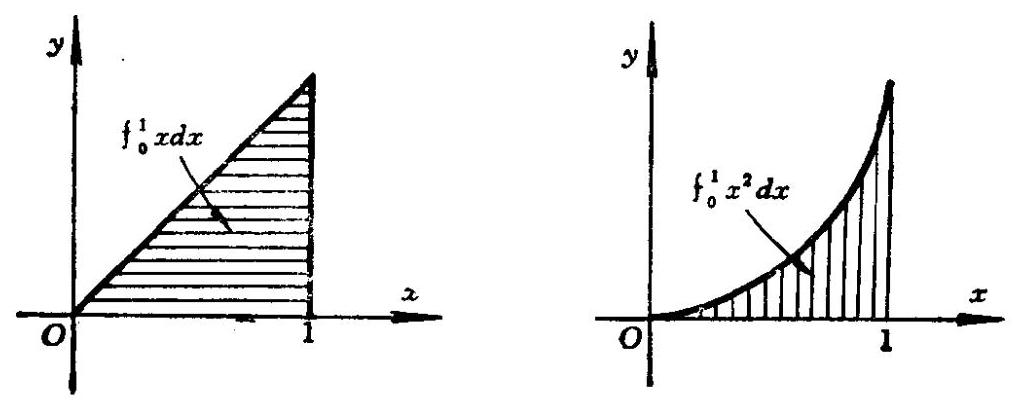
\includegraphics[max width=0.9\textwidth]{images/bo_d25ksc77aajc738obdgg_241_348_1482_1015_401_0.jpg}
\end{center}
\hspace*{3em} 

图 5-9

例2 证明: $\forall a > 0,b > 0$ ,
$${\int }_{1}^{b}\frac{1}{x}{dx} = {\int }_{a}^{ab}\frac{1}{x}{dx}.$$

首先设 $b > 1$ : 由于函数 $x \mapsto  f\left( x\right)  = \frac{1}{x},x \in  \rbrack 0, + \infty \lbrack$ 连续, 故 $f$ 在 $\left\lbrack  {1,b}\right\rbrack$ 及 $\left\lbrack  {a,{ab}}\right\rbrack$ 可积,根据上述推论我们有
\begin{align*}
	&{\int }_{1}^{b}\frac{1}{x}{dx} = \mathop{\lim }\limits_{{n \rightarrow   + \infty }}\mathop{\sum }\limits_{{i = 0}}^{{n - 1}}\frac{1}{1 + i\frac{b - 1}{n}} \cdot  \frac{b - 1}{n}\\
	&= \mathop{\lim }\limits_{{n \rightarrow   + \infty }}\mathop{\sum }\limits_{{i = 0}}^{{n - 1}}\frac{1}{a + i\frac{{ab} - a}{n}} \cdot  \frac{{ab} - a}{n}\\
	&= {\int }_{a}^{ab}\frac{1}{x}{dx}.
\end{align*}

再设 $b < 1$ : 根据约定, ${\int }_{1}^{b}\frac{1}{x}{dx} =  - {\int }_{b}^{1}\frac{1}{x}{dx}$ ,因此由 $b > 1$ 时所证结论我们有
\begin{align*}
	&{\int }_{1}^{b}\frac{1}{x}{dx} =  - {\int }_{b}^{1}\frac{1}{x}{dx} =  - {\int }_{b}^{b \cdot  \frac{1}{b}}\frac{1}{x}{dx} =  - {\int }_{1}^{\frac{1}{b}}\frac{1}{x}{dx}\\
	&=  - {\int }_{ab}^{{ab} \cdot  \frac{1}{b}}\frac{1}{x}{dx} =  - {\int }_{ab}^{a}\frac{1}{x}{dx} = {\int }_{a}^{ab}\frac{1}{x}{dx}.
\end{align*}

最后设 $b = 1$ : 这时,由约定 ${\int }_{1}^{1}\frac{1}{x}{dx} = {\int }_{a}^{a}\frac{1}{x}{dx} = 0$ .

例 3 证明实数序列 $\left\langle  {\frac{1}{{n}^{3}}\mathop{\sum }\limits_{{k = 0}}^{{n - 1}}{k}^{2}\sin \frac{k\pi }{n}}\right\rangle$ 收敛,并求其极限.

事实上,考虑函数 $x \mapsto  f\left( x\right)  = {x}^{2}\sin {\pi x},x \in  \left\lbrack  {0,1}\right\rbrack$ . 它在 $\left\lbrack  {0,1}\right\rbrack$ 上连续,因此 $f$ 在 $\left\lbrack  {0,1}\right\rbrack$ 上Riemann 可积. 根据上述推论, 我们有
\begin{align*}
	&{\int }_{0}^{1}f\left( x\right) {dx} = \mathop{\lim }\limits_{{n \rightarrow   + \infty }}\mathop{\sum }\limits_{{k = 0}}^{{n - 1}}f\left( {0 + k\frac{1}{n}}\right) \frac{1}{n}\\
	&= \mathop{\lim }\limits_{{n \rightarrow  \cdots \infty }}\mathop{\sum }\limits_{{k = 0}}^{{n - 1}}{\left( \frac{k}{n}\right) }^{2}\sin \frac{k\pi }{n} \cdot  \frac{1}{n}\\
	&= \mathop{\lim }\limits_{{n \rightarrow   + \infty }}\frac{1}{{n}^{3}}\mathop{\sum }\limits_{{k = 0}}^{{n - 1}}{k}^{2}\sin \frac{k\pi }{n}.
\end{align*}

此即表明实数序列 $\left\langle  {\frac{1}{{n}^{3}}\mathop{\sum }\limits_{{k = 0}}^{{n - 1}}{k}^{2}\sin \frac{k\pi }{n}}\right\rangle$ 收敛,其极限为

${\int }_{0}^{1}{x}^{2}\sin {\pi xdx}$

\section*{习 题}

1. 设 $f : \mathbf{R} \rightarrow  \mathbf{R}$ 在任意有限区间 $\left\lbrack  {\alpha ,\beta }\right\rbrack$ 上Riemann可积,直接用 Riemann 积分定义证明下列等式:

1) ${\int }_{a}^{b}f\left( x\right) {dx} = {\int }_{a + c}^{b + c}f\left( {x - c}\right) {dx},\forall c \in  \mathbf{R}$ .

2) ${\int }_{ac}^{bc}f\left( x\right) {dx} = c{\int }_{a}^{b}f\left( {cx}\right) {dx},\forall c \in  \mathbf{R}$ .

2 . 证明定理 $5 \cdot  3 \cdot  1$ 的推论.

3. 证明下列各极限存在, 并求其极限.

1) $\mathop{\lim }\limits_{{n \rightarrow   + \infty }}\left( {\frac{1}{n + 1} + \frac{1}{n + 2} + \cdots  + \frac{1}{n + n}}\right)$ .

2) $\mathop{\lim }\limits_{{n \rightarrow   + \infty }}\left( {\frac{n}{{n}^{2} + 1} + \frac{n}{{n}^{2} + 2} + \cdots  + \frac{n}{{n}^{2} + n}}\right)$ .

3) $\mathop{\lim }\limits_{{n \rightarrow   + \infty }}\frac{1}{n}\left( {\sin \frac{\pi }{n} + \sin \frac{2\pi }{n} + \cdots  + \sin \frac{n\pi }{n}}\right)$ .

4) $\mathop{\lim }\limits_{{n \rightarrow   + \infty }}\left( {\frac{{1}^{\alpha }}{{n}^{\alpha  + 1}} + \frac{{2}^{\alpha }}{{n}^{\alpha  + 1}} + \cdots  + \frac{{n}^{\alpha }}{{n}^{\alpha  + 1}}}\right) \;\left( {\alpha  > 0}\right)$ .

5) $\mathop{\lim }\limits_{{n \rightarrow   + \infty }}\sin \frac{\pi }{n}\mathop{\sum }\limits_{{k = 0}}^{{n - 1}}\frac{1}{2 + \cos \frac{k\pi }{n}}$ .

4. 设 $f : \left\lbrack  {a,b}\right\rbrack   \rightarrow  \mathrm{R}$ 是任一有界函数. $\sigma  = \left( {{a}_{0},{a}_{1},\cdots ,{a}_{n}}\right)$ 是 $\left\lbrack  {a,b}\right\rbrack$ 的任一分割. 令
\begin{align*}
	&{m}_{i} = \mathop{\inf }\limits_{{x \in  \left\lbrack  {{a}_{i};{a}_{i + 1}}\right\rbrack  }}f\left( x\right) ,\;{M}_{i} = \mathop{\sup }\limits_{{x \in  \left\lbrack  {{a}_{i};{a}_{i + 1}}\right\rbrack  }}f\left( x\right) ,\\
	&{D}_{i}\left( {f,\sigma }\right)  = \mathop{\sum }\limits_{{i = 0}}^{{n - 1}}{m}_{i}\left( {{a}_{i + 1} - {a}_{i}}\right) ,\;{D}_{s}\left( {f,\sigma }\right)  = \mathop{\sum }\limits_{{i = 0}}^{{n - 1}}{M}_{i}\left( {{a}_{i + 1} - {a}_{i}}\right) .
\end{align*}

我们分别称 ${D}_{i}\left( {f,\sigma }\right)$ 与 ${D}_{s}\left( {f,\sigma }\right)$ 为 $f$ 关于 $\sigma$ 的Darboux下和与Darboux上和. 证明下述结论等价:

1) $f$ 在 $\left\lbrack  {a,b}\right\rbrack$ 上Riemann可积.

2) $\forall \varepsilon  > 0,\exists \sigma$ 使得 $0 \leq  D,\left( {f,\sigma }\right)  - {D}_{i}\left( {f,\sigma }\right)  < \varepsilon$ .

5. 我们用 $\mathcal{A}$ 表示 $\left\lbrack  {a,b}\right\rbrack$ 的所有分割的集合. $\forall {\sigma }_{1},{\sigma }_{2} \in  \mathcal{A}$ ,我们称 ${\sigma }_{2}$ 比 ${\sigma }_{1}$ 细,如果 ${\sigma }_{1}$ 的分点也是 ${\sigma }_{2}$ 的分点. 这时记为 ${\sigma }_{1} \prec  {\sigma }_{2}$ .

这个题目的目的是证明:
$$\forall \sigma ,{\sigma }^{\prime } \in  \mathcal{A},{D}_{i}\left( {f,\sigma }\right)  \leq  {D}_{s}\left( {f,{\sigma }^{\prime }}\right) .$$

1) 证明: $\forall \sigma  \in  \mathcal{A}$ ,若 ${\sigma }^{\prime }$ 是比 $\sigma$ 多一个分点的分割,则
$${D}_{i}\left( {f,\sigma }\right)  \leq  {D}_{i}\left( {f,{\sigma }^{\prime }}\right) ,{D}_{s}\left( {f,{\sigma }^{\prime }}\right)  \leq  {D}_{s}\left( {f,\sigma }\right) .$$

2) 证明: 若 $\sigma ,{\sigma }^{\prime } \in  \mathcal{A}$ 且 $\sigma  \prec  {\sigma }^{\prime }$ ,则
$${D}_{i}\left( {f,\sigma }\right)  \leq  {D}_{i}\left( {f,{\sigma }^{\prime }}\right) ,{D}_{s}\left( {f,{\sigma }^{\prime }}\right)  \leq  {D}_{s}\left( {f,\sigma }\right) .$$

3) 证明: 若 $\sigma ,{\sigma }^{\prime } \in  \mathcal{A}$ ,则 $\sigma  \prec  \sigma  \smallsetminus  {\sigma }^{\prime },{\sigma }^{\prime } \prec  \sigma  \smallsetminus  {\sigma }^{\prime }$ .

4) 由此推得: ${D}_{i}\left( {f,\sigma }\right)  \leq  {D}_{s}\left( {f,{\sigma }^{\prime }}\right)$ .

6. 设 $f : \left\lbrack  {a,b}\right\rbrack   \rightarrow  \mathrm{R}$ 是任一有界函数,令
$$E = \left\{  {{D}_{i}\left( {f,\sigma }\right)  \mid  \sigma  \in  \mathcal{A}}\right\}  ,F = \left\{  {{D}_{s}\left( {f,\sigma }\right)  \mid  \sigma  \in  \mathcal{A}}\right\}  .$$

1) 证明: $E$ 是上有界集, $F$ 是下有界集.

2) 若令 ${D}_{i}\left( f\right)  = \sup E,{D}_{s}\left( f\right)  = \inf F$ ,则 ${D}_{i}\left( f\right)  \leq  {D}_{s}\left( f\right)$ .

3) 证明: $f$ 在 $\left\lbrack  {a,b}\right\rbrack$ 上的上积分 $S\left( f\right)$ 与下积分 $i\left( f\right)$ (上、下积分定义见§2习题5)满足下述等式:
$$i\left( f\right)  = {D}_{i}\left( f\right) ,\;S\left( f\right)  = {D}_{s}\left( f\right) .$$

7. 设 $f : \left\lbrack  {a,b}\right\rbrack   \rightarrow  \mathrm{R}$ 是任一有界函数. 证明下述各结论等价:

1) $f \in  \mathcal{R}\left\lbrack  {a,b}\right\rbrack$ .

2) $\mathop{\lim }\limits_{\mathcal{B}}S\left( {f,\sigma ,\xi }\right)  = A\left( {A \in  R}\right)$ .

3) ${D}_{i}\left( f\right)  = {D}_{s}\left( f\right)$ .

4) $i\left( f\right)  = S\left( f\right)$ .

8. 设 $f : \left\lbrack  {a,b}\right\rbrack   \rightarrow  \left\lbrack  {c,d}\right\rbrack$ 是任一严格单调上升的连续函数. ${f}^{-1} : \lbrack c$ , $d\rbrack  \rightarrow  \left\lbrack  {a,b}\right\rbrack$ 是 $f$ 的反函数.

1) 设 $\sigma  = \left( {{c}_{0},{c}_{1},\cdots ,{c}_{n}}\right)$ 是 $\left\lbrack  {c,d}\right\rbrack$ 的任一分割, ${\sigma }^{-1} = \left( {{f}^{-1}\left( {c}_{0}\right) }\right.$ ,

$\left. {{f}^{-1}\left( {c}_{1}\right) ,\cdots ,{f}^{-1}\left( {c}_{n}\right) }\right)$ 是对应于 $\sigma$ 的 $\left\lbrack  {a,b}\right\rbrack$ 的一个分割. 证明:
$${D}_{i}\left( {{f}^{-1},\sigma }\right)  + {D}_{s}\left( {f,{\sigma }^{-1}}\right)  = {bd} - {ac}.$$

2) 利用上述等式, 证明:
$${\int }_{c}^{d}{f}^{-1}\left( x\right) {dx} + {\int }_{a}^{b}f\left( x\right) {dx} = {bd} - {ac}.$$

3) 利用 2 ) 的公式计算积分 ${\int }_{0}^{1}\sqrt{x}{dx}$ .

9. 设 ${f}_{1}\left\lbrack  {a,b}\right\rbrack   \rightarrow  R$ 是任一有界 函 数。这个题目的目的是要证明: 若 $f \in  \mathcal{X}\left\lbrack  {a,b}\right\rbrack$ ,则 $f$ 在 $\left\lbrack  {a,b}\right\rbrack$ 上的连续点集是一个无限集.

1) 设 $\sigma  = \left( {{a}_{0},{a}_{1},\cdots ,{a}_{m}}\right)$ 是 $\left\lbrack  {a,b}\right\rbrack$ 的一个分割,使得 $0 \leq  {D}_{s}\left( {f,\sigma }\right)  \smallsetminus$  ${D}_{i}\left( {f,\sigma }\right)  < b - a$ . 证明: 存在 $i \in  \{ 0,1,\cdots ,m - 1\}$ 使得
$$0 \leq  {M}_{i} - {m}_{i} < 1\text{ 这里 }{m}_{i} = \mathop{\inf }\limits_{{x \in  \left\lbrack  {{a}_{i} : {a}_{i + 1}}\right\rbrack  }}f\left( x\right) ,{M}_{i} = \mathop{\sup }\limits_{{x \in  \left\lbrack  {{a}_{i} : {a}_{i + 1}}\right\rbrack  }}f\left( x\right) .$$

2) 证明: 存在实数 ${a}_{1},{b}_{1}$ 使得 $a < {a}_{1} < {b}_{1} < b$ ,并且
$$0 \leq  \mathop{\sup }\limits_{{x \in  \left\lbrack  {{a}_{1};{b}_{1}}\right\rbrack  }}f\left( x\right)  - \mathop{\inf }\limits_{{x \in  \left\lbrack  {{a}_{1};{b}_{1}}\right\rbrack  }}f\left( x\right)  < 1.$$

3) 证明: 存在实数 ${a}_{2},{b}_{2}$ 使得 $a < {a}_{1} < {a}_{2} < {b}_{2} < {b}_{1} < b$ ,并且
$$0 \leq  \mathop{\sup }\limits_{{x \in  \left\lbrack  {{a}_{2};{b}_{2}}\right\rbrack  }}f\left( x\right)  - \mathop{\inf }\limits_{{x \in  \left\lbrack  {{a}_{2};{b}_{2}}\right\rbrack  }}f\left( x\right)  < \frac{1}{2}.$$

4) 将此过程无限地继续下去,我们得到一闭区间族 ${\left\{  \left\lbrack  {a}_{n},{b}_{n}\right\rbrack  \right\}  }_{n \in  \mathbf{N}}$ , 使得
\begin{align*}
	&\left\lbrack  {{a}_{n + 1},{b}_{n + 1}}\right\rbrack   \subset  \left\lbrack  {{a}_{n},{b}_{n}}\right\rbrack  ,0 \leq  \mathop{\sup }\limits_{{x \in  \left\lbrack  {{a}_{n};{b}_{n}}\right\rbrack  }}f\left( x\right)  - \mathop{\inf }\limits_{{x \in  \left\lbrack  {{a}_{n};{b}_{n}}\right\rbrack  }}f\left( x\right)  < \frac{1}{n},\\
	&\forall n \in  \mathbf{N}\text{ . }
\end{align*}

由此推得存在一点 $x \in  \left\lbrack  {a,b}\right\rbrack$ 使得 $f$ 在 $x$ 处连续.

5) 证明: $f$ 在 $\left\lbrack  {a,b}\right\rbrack$ 上有无限多个连续点.

6) 假设 $f \in  \mathcal{B}\left\lbrack  {a,b}\right\rbrack$ ,并且 $f > 0$ ,证明 ${\int }_{a}^{b}f\left( x\right) {dx} > 0$ .

\section{基本初等函数的定义}

现在我们利用积分函数来定义对数函数、指数函数、幂函数等基本初等函数, 并研究它们的基本性质及其图形.

在定义基本初等函数之前, 我们先介绍如下概念.

\section*{1. 函数图形的无穷远分支及其渐近线}

定义 设 $X \subset  \mathbf{R}$ 是任一非空集合, $f : X \rightarrow  \mathbf{R}$ 是任一函数.

1) 若 $+ \infty$ 或 $- \infty$ 是 $X$ 的聚点,并且存在直线 $L : y = {kx} + b$ 使得
$$f\left( x\right)  - \left( {{kx} + b}\right)  \rightarrow  0\;\left( {x \rightarrow   + \infty \text{ 或 } - \infty }\right) ,$$

则我们称函数 $f$ 的图形 $\operatorname{Gr}\left( f\right)$ 有无穷远分支 ${\Gamma }_{+\infty }$ 或 ${\Gamma }_{-\infty }$ ,而直线 $L$ 称为此无穷远分支的渐近线,特别地,当 $k = 0$ 时,直线 $L : y = b$ 又称为水平渐近线.

2) 若 $a \in  \mathbf{R}$ 是 $X$ 的有限聚点,使得
$$f\left( x\right)  \rightarrow   + \infty \text{ 或 } - \infty \;\left( {x \rightarrow  {a}^{ + }\text{ 或 }x \rightarrow  {a}^{ - }}\right) ,$$

则我们称函数 $f$ 的图形 $\operatorname{Gr}\left( f\right)$ 有无穷远分支 ${\Gamma }_{{a}^{ + }}$ 或 ${\Gamma }_{{a}^{ - }}$ ,而直线 $x$  $= a$ 称为此无穷远分支的垂直渐近线.

由上述渐近线的定义可知,直 线 $L : y = {kx} + b$ 是无穷远分支 ${\Gamma }_{+\infty }$ 或 ${\Gamma }_{-\infty }$ 的渐近线,当且仅当:
$$k = \mathop{\lim }\limits_{{x \rightarrow   + \infty }}\frac{f\left( x\right) }{x},\;b = \mathop{\lim }\limits_{{x \rightarrow   + \infty }}\left\lbrack  {f\left( x\right)  - {kx}}\right\rbrack  .$$

\section*{2. 基本初等函数的定义及性质}

\section*{1)自然对数函数}

由于函数 $x \mapsto  \frac{1}{x},x \in  \rbrack 0, + \infty \lbrack$ 连续,故它的积分函数 $x \mapsto  {\int }_{1}^{x}\frac{1}{t}{dt},x \in  \rbrack 0, + \infty \lbrack$ 存在.

定义 函数 $x \mapsto  {\int }_{1}^{x}\frac{1}{t}{dt},x \in  \rbrack 0, + \infty \lbrack$ 称为自然对数函数,记为 $\log \left( \text{ 或 ln }\right) .\forall x \in  \rbrack 0, + \infty \lbrack ,\log x$ 称为 $x$ 的自然对数. 于提
\begin{align*}
	&\log x = {\int }_{1}^{x}\frac{1}{t}{dt},\;\forall x \in  \rbrack 0, + \infty \lbrack .\\
	&\log 1 = 0\text{ . }
\end{align*}

自然对数函数的基本性质可综述如下.

定理 $5 \cdot  4 \cdot  1\;1)\;\forall x,y \in  \rbrack 0, + \infty \lbrack ,\forall n \in  \mathbf{Z}$ ,
\begin{align*}
	&\log {xy} = \log x + \log y\\
	&{\log }_{y}^{x}\frac{x}{y} = \log x - \log y\\
	&\log {x}^{n} = n\log x.
\end{align*}

2 ) $\log$ 是严格单调上升的连续函数,并且
$$\mathop{\lim }\limits_{{x \rightarrow  {0}^{ + }}}\log x =  - \infty ,\mathop{\lim }\limits_{{x \rightarrow   + \infty }}\log x =  + \infty .$$

因此 $\log$ 是从乘法群 $\left( {{\mathbf{R}}_{ * }^{ + }, \cdot  }\right)$ 到加法群 $\left( {\mathbf{R}, + }\right)$ 上的同构映射.

3) $\log$ 的图形有无穷远分支 ${\Gamma }_{0} +$ 及垂直渐近线 $x = 0$ .

证明 1) $\forall x,y \in  \rbrack 0, + \infty \lbrack$ ,由 $§3$ 例 2 知
\begin{align*}
	&\log {xy} = {\int }_{1}^{xy}\frac{1}{t}{dt} = {\int }_{1}^{x}\frac{1}{t}{dt} + {\int }_{x}^{xy}\frac{1}{t}{dt}\\
	&= {\int }_{1}^{x}\frac{1}{t}{dt} + {\int }_{1}^{y}\frac{1}{t}{dt}\\
	&= \log x + \log y.
\end{align*}

特别地取 $y = \frac{1}{x}$ ,我们得到
$$0 = \log 1 = \log x \cdot  \frac{1}{x} = \log x + \log \frac{1}{x}.$$

从而 $\log \frac{1}{x} =  - \log x$ ,因此
$$\log \frac{x}{y} = \log x + \log \frac{1}{y} = \log x - \log {y}_{ \bullet  }$$

现在设 $n \in  \mathbf{Z}$ .

若 $n \in  \mathbf{N}$ : 则 $\log {x}^{n} = \log x \cdot  x \cdot  \cdots  \cdot  x$
\begin{align*}
	&= \log x + \log x + \cdots  + \log x\\
	&= n\log x\text{ . }
\end{align*}

若 $- n \in  \mathbf{N}$ : 则令 $m =  - n$ . 从而
\begin{align*}
	&\log {x}^{n} = \log {x}^{m} = \log \frac{1}{{x}^{m}}\\
	&=  - \log {x}^{m} =  - m\log x = n\log x.
\end{align*}

若 $n = 0$ : 则
$$\log {x}^{0} = \log 1 = 0 = 0 \cdot  \log x.$$

因此 $\forall n \in  \mathbf{Z},\log {x}^{n} = n\log x$ .

2) 因为积分函数连续,所以自然对数函数 $\log$ 在 $\rbrack 0, + \infty \lbrack$ 上连续.

现在设 ${x}_{1},{x}_{2} \in  \rbrack 0, + \infty \lbrack$ ,并且 ${x}_{1} < {x}_{2}$ . 则
$$\log {x}_{2} - \log {x}_{1} = {\int }_{{x}_{1}}^{{x}_{2}}\frac{1}{t}{dt} > 0.$$

因此 $\log {x}_{2} > \log {x}_{1}$ ,从而 $\log$ 在 $\rbrack 0, + \infty \lbrack$ 上严格单调上升.

另一方面, 由于
$$\log {2}^{n} = n\log 2,\log 2 > \log 1 = 0,$$

故
\begin{align*}
	&\mathop{\lim }\limits_{{x \rightarrow   + \infty }}\log x =  + \infty \text{ ; }\\
	&\mathop{\lim }\limits_{{x \rightarrow  {0}^{ + }}}\log x =  - \mathop{\lim }\limits_{{x \rightarrow  {0}^{ + }}}\log \frac{1}{x} =  - \mathop{\lim }\limits_{{y \rightarrow   + \infty }}\log y =  - \infty .
\end{align*}

由此并结合性质 1 )知 $\log$ 是从乘法群 $\left( {{\mathbf{R}}_{ * }^{ * }, \cdot  }\right)$ 到加法群 $\left( {\mathbf{R}, + }\right)$ 上的同构映射.

3) 因为 $\mathop{\lim }\limits_{{x \rightarrow  {0}^{ + }}}\log x =  - \infty$ ,故 $\log$ 的图形有无穷远分支 ${\Gamma }_{{0}^{ + }}$ , 并且负 $y$ 轴是它的垂直渐近线.

根据上述分析,自然对数函数 $\log$ 的图形可描述如下:

附注 由于 $\log$ 是从 $\rbrack 0$ , $+ \infty \lbrack$ 到 $\rbrack  - \infty , + \infty \lbrack$ 上的严格单调上升连续函数,故存在唯一的 $\bar{x} \in  \rbrack 0, + \infty \lbrack$ 使得 $\log \bar{x} = 1$ ,我们习惯地记 $\bar{x} = e$ ,于是
$$\log e = 1\text{ . }$$

\begin{center}
	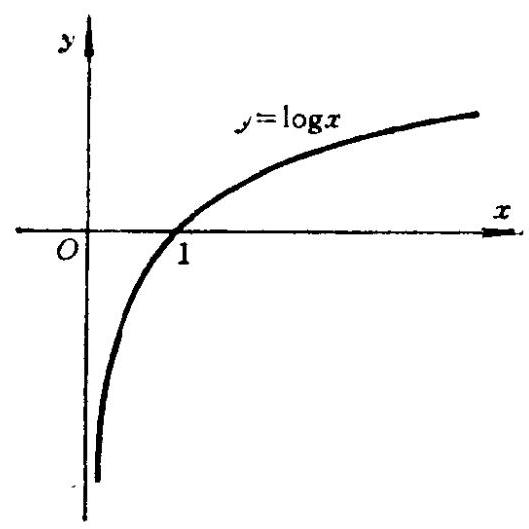
\includegraphics[max width=0.4\textwidth]{images/bo_d25ksc77aajc738obdgg_249_598_264_529_529_0.jpg}
\end{center}
\hspace*{3em} 

图 5-10

2) 以 $a\left( {0 < a \neq  1}\right)$ 为底的对数函数

由于 $0 < a \neq  1$ ,故 $\log a \neq  0$ .

定义 函数 $x \mapsto  \frac{\log x}{\log a},x \in  \rbrack 0, + \infty \lbrack$ 称为以 $a$ 为底的对数函数,记为 ${\log }_{a}.\forall x \in  \rbrack 0, + \infty \left\lbrack  {,{\log }_{a}x}\right.$ 称为 $x$ 的以 $a$ 为底的对数.

若 $a = {10}$ ,则 ${\log }_{a}x$ 称为 $x$ 的常用对数.

由于 $\log e = 1$ ,故
$${\log }_{e}x = \log x\;\left( {x \in  \rbrack 0, + \infty \lbrack }\right) .$$

因此自然对数函数 $\log$ 就是以 $e$ 为底的对数函数.

利用 ${\log }_{a}$ 的定义及定理 $5 \cdot  4 \cdot  1$ 可证明关于 ${\log }_{a}$ 的下述性质.

定理 $5 \cdot  4 \cdot  2\;1)\;\forall x,y \in  \rbrack 0, + \infty \lbrack ,\forall n \in  \mathbf{Z}$ .
\begin{align*}
	&{\log }_{a}{xy} = {\log }_{a}x + {\log }_{a}y,\\
	&{\log }_{a}\frac{x}{y} = {\log }_{a}x - {\log }_{a}y,\\
	&{\log }_{a}{x}^{n} = n{\log }_{a}x.
\end{align*}

2) 若 $a > 1\left( {0 < a < 1}\right)$ ,则 ${\log }_{a}$ 是严格单调上升 (下降) 的连续函数, 并且
\begin{align*}
	&\mathop{\lim }\limits_{{x \rightarrow  {0}^{ + }}}{\log }_{a}x =  - \infty ,\mathop{\lim }\limits_{{x \rightarrow   + \infty }}{\log }_{a}x =  + \infty .\\
	&\left( {\mathop{\lim }\limits_{{x \rightarrow  {0}^{ + }}}{\log }_{a}x =  + \infty ,\mathop{\lim }\limits_{{x \rightarrow   + \infty }}{\log }_{a}x =  - \infty .}\right)
\end{align*}

因此 ${\log }_{a}$ 是从乘法群 $\left( {{\mathbf{R}}_{ * }^{ + }, \cdot  }\right)$ 到加法群 $\left( {\mathbf{R}, + }\right)$ 上的同构映射.

3) 当 $a > 1\left( {0 < a < 1}\right)$ 时, ${\log }_{a}$ 的图形有无穷远分支 ${\Gamma }_{{0}^{ + }}$ ,并且负 (正) $y$ 轴是 ${\Gamma }_{0} +$ 的垂直渐近线.

定理的证明留给读者作为练习.

${\log }_{a}$ 的图形如图 5-11 所示.

\begin{center}
	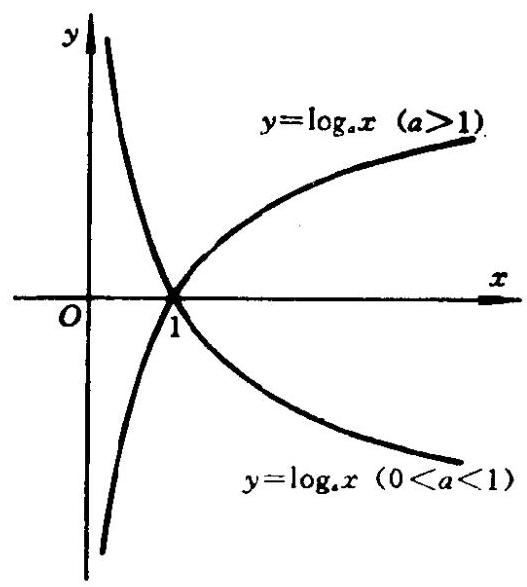
\includegraphics[max width=0.4\textwidth]{images/bo_d25ksc77aajc738obdgg_250_458_710_527_587_0.jpg}
\end{center}
\hspace*{3em} 

图 5-11

\section*{3 )以 $e$ 为底的指数函数}

由于自然对数函数 $x \mapsto  \log x,x \in  \rbrack 0, + \infty \left\lbrack  \right.$ 是从 $\rbrack 0, + \infty \lbrack$ 到 $\mathbf{R}$ 上的严格单调上升的连续函数,根据定理 $4 \cdot  7 \cdot  1$ 知,它有反函数存在,并且是从 $\mathbf{{R到}}\rbrack 0, + \infty \lbrack$ 上的严格单调上升的连续函数. 我们记这个反函数为:
$$x \mapsto  \exp x,x \in  \mathbf{R}.$$

于是我们有
\begin{align*}
	&\log \left( {\exp x}\right)  = x,\;\forall x \in  \mathbf{R}.\\
	&\exp \left( {\log x}\right)  = x,\;\forall x \in  {\mathbf{R}}_{ * }^{ + }.
\end{align*}

现在我们特别地取 $x = n \in  \mathbf{Z}$ ,由 $\log$ 的性质有
$$\log \left( {\exp n}\right)  = n = n\log e = \log {e}^{n}.$$

从而
$$\exp n = {e}^{n}\text{ . }$$

这启发我们引入下述定义及记号.

定义 $\forall x \in  \mathbf{R}$ ,我们令
$${e}^{x} \triangleq  \exp x.$$

函数 $x \mapsto  {e}^{x},x \in  \mathbf{R}$ 称为以 $e$ 为底 $x$ 为指数的指数函数.

关于此函数的性质, 我们有下述定理.

定理 $5 \cdot  4 \cdot  3\;1)\;\forall x,y \in  \mathbf{R}$ .
\begin{align*}
	&{e}^{x + y} = {e}^{x} \cdot  {e}^{y},{e}^{x - y} = \frac{{e}^{x}}{{e}^{y}},\\
	&{e}^{0} = 1,y = {e}^{x} \Leftrightarrow  x = \log y.
\end{align*}

2) $x \mapsto  {e}^{x},x \in  \mathbf{R}$ 是严格单调上升的连续函数并且
$$\mathop{\lim }\limits_{{x \rightarrow   - \infty }}{e}^{x} = 0,\mathop{\lim }\limits_{{x \rightarrow   + \infty }}{e}^{x} =  + \infty .$$

因此它是从加法群 $\left( {\mathbf{R}, + }\right)$ 到乘法群 $\left( {{\mathbf{R}}_{ * }^{ + }, \cdot  }\right)$ 上的同构映射.

3) 此函数的图形有无穷远分支 ${\Gamma }_{-\infty }$ ,并且 $y = 0$ 是 ${\Gamma }_{-\infty }$ 的水平渐近线.

证明 1) $\forall x,y \in  \mathbf{R}$ ,由于 $\log \left( {e}^{x}\right)  = x$ ,故
\begin{align*}
	&\log \left( {e}^{x + y}\right)  = x + y,\;\log \left( {e}^{x - y}\right)  = x - y,\\
	&\log \left( {{e}^{x} \cdot  {e}^{y}}\right)  = \log {e}^{x} + \log {e}^{y} = x + y,\\
	&\log \frac{{e}^{x}}{{e}^{y}} = \log {e}^{x} - \log {e}^{y} = x - y.
\end{align*}

由 $\log$ 的单射性推知,
$${e}^{x + y} = {e}^{x} \cdot  {e}^{y},{e}^{x - y} = \frac{{e}^{x}}{{e}^{y}},{e}^{0} = 1.$$

同样由 $\log {e}^{x} = x$ 推得
$$y = {e}^{x} \Leftrightarrow  \log y = \log {e}^{x} = x.$$

2) 由于 $x \mapsto  {e}^{x},x \in  \mathbf{R}$ 是自然对数函数 $\log$ 的反函数,故它是从 $\mathbf{R}$ 到 ${\mathbf{R}}_{ * }^{ * }$ 上的严格单调上升的连续函数,从而
$$\mathop{\lim }\limits_{{x \rightarrow   - \infty }}{e}^{x} = 0,\mathop{\lim }\limits_{{x \rightarrow   + \infty }}{e}^{x} =  + \infty .$$

因此结合性质 1 )知以 $e$ 为底的 指数 函数是从加法群 $(\mathbf{R}$ , $+ )$ 到乘法群 $\left( {{\mathbf{R}}_{ * }^{ + }, \cdot  }\right)$ 上的同构映射.

3) 由于 $\mathop{\lim }\limits_{{x \rightarrow   - \infty }}{e}^{x} = 0$ ,故此函数的图形有无穷远分支 ${\Gamma }_{-\infty }$ ,它以 $y = 0$ 为其水平渐近线.

由于以 $e$ 为底的指数函数是自然对数函数的反函数,故这两个函数的图形关于直线 $y = x$ 对称,从而由 $\log$ 的图形得到函数 $x$  $\mapsto  {e}^{x},x \in  \mathbf{R}$ 的图形,如图 5-12 所示.

\begin{center}
	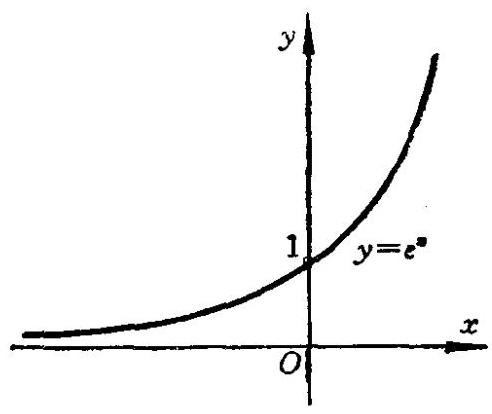
\includegraphics[max width=0.4\textwidth]{images/bo_d25ksc77aajc738obdgg_252_386_818_492_414_0.jpg}
\end{center}
\hspace*{3em} 

图 5-12

4) 以 $a\left( {a > 0}\right)$ 为底的指数函数

定义 $\forall x \in  \mathbf{R}$ ,令
$${a}^{x} \bigtriangleup  {e}^{x\log a}\text{ . }$$

函数 $x \mapsto  {a}^{x},x \in  \mathbf{R}$ 称为以 $a$ 为底 $x$ 为指数的指数函数.

由以 $e$ 为底的指数函数的性质可推得以 $a$ 为底的指数函数的下述性质.

定理 $5 \cdot  4 \cdot  4\;1)\;\forall x,y \in  \mathrm{R},$
\begin{align*}
	&\log {a}^{x} = x\log a,\\
	&{a}^{x + y} = {a}^{x} \cdot  {a}^{y},\\
	&{a}^{-x} = \frac{1}{{a}^{x}} = {\left( \frac{1}{a}\right) }^{x},\\
	&{a}^{x - y} = \frac{{a}^{x}}{{a}^{y}},\;{\left( {a}^{x}\right) }^{y} = {a}^{xy},\\
	&{\left( ab\right) }^{x} = {a}^{x} \cdot  {b}^{x}\left( {b > 0}\right) ,y = {a}^{x} \Leftrightarrow  x = {\log }_{a}y.
\end{align*}

2) 若 $a > 1$ ,则 $x \mapsto  {a}^{x},x \in  \mathbf{R}$ 是严格单调上升的连续函数, 并且
$$\mathop{\lim }\limits_{{x \rightarrow   - \infty }}{a}^{x} = 0,\mathop{\lim }\limits_{{x \rightarrow   + \infty }}{a}^{x} =  + \infty .$$

若 $0 < a < 1$ ,则 $x \mapsto  {a}^{x},x \in  \mathbf{R}$ 是严格单调下降的连续函数, 并且
$$\mathop{\lim }\limits_{{x \rightarrow   - \infty }}{a}^{x} =  + \infty ,\mathop{\lim }\limits_{{x \rightarrow   + \infty }}{a}^{x} = 0.$$

若 $a = 1$ ,则 ${1}^{x} = 1,\forall x \in  \mathbf{R}$ .

因此 $\forall a > 0$ 且 $a \neq  1,x \mapsto  {a}^{x},x \in  \mathbf{R}$ 是从加法 群 $\left( {\mathbf{R}, + }\right)$ 到乘法群 $\left( {{\mathbf{R}}_{ * }^{ + }, \cdot  }\right)$ 上的同构映射.

3) 若 $a > 1\left( {0 < a < 1}\right)$ ,函数 $x \mapsto  {a}^{x},x \in  \mathbf{R}$ 的图形有无穷. 远分支 ${\Gamma }_{-\infty }\left( {\Gamma }_{+\infty }\right)$ ,它以 $y = 0$ 为水平渐近线.

定理的证明留给读者.

由性质 1 )可知,函数 $x \mapsto  {a}^{x},x \in  \mathbf{R}$ 是对数函数 $x \mapsto$  ${\log }_{a}x,x \in  {\mathbf{R}}_{ * }^{ + }$ 的反函数,故它的图形如图 5-13 所示.

\begin{center}
	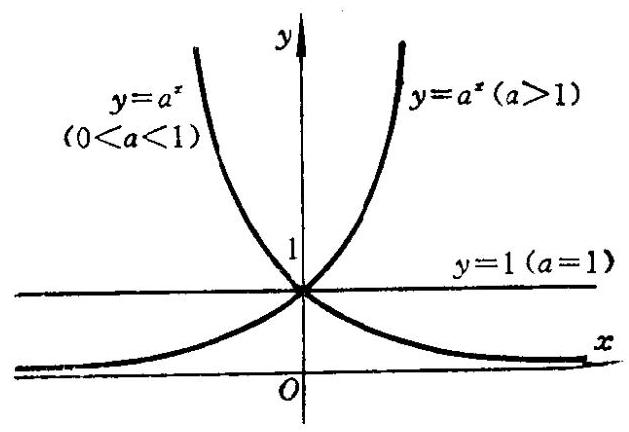
\includegraphics[max width=0.5\textwidth]{images/bo_d25ksc77aajc738obdgg_253_501_1402_629_432_0.jpg}
\end{center}
\hspace*{3em} 

图 5-13

5)幂函数

我们知道

i) 若 $n \in  \mathbf{N}$ ,则 $\forall x \in  \mathbf{R},{x}^{n} \triangleq  x \cdot  x\cdots  \cdot  x$ .

ii) 若 $- n \in  \mathbf{N}$ . 则 $\forall x \in  \mathbf{R} - \{ 0\} ,{x}^{n} \triangleq  \frac{1}{{x}^{-n}}$
$$= {\left( \frac{1}{x}\right) }^{-n}$$

iii) 若 $n = 0$ ,则 $\forall x \in  \mathbf{R} - \{ 0\} ,{x}^{0} = 1$ .

下面我们考虑 $\alpha  \in  \mathbf{R} - \mathbf{Z}$ .

定义 设 $\alpha  \in  \mathbf{R} - \mathbf{Z},\forall x \in  \rbrack 0, + \infty \lbrack$ ,令
$${x}^{a} \triangleq  {e}^{a\log x}.$$

函数 $x \mapsto  {x}^{ * },x \in  \rbrack 0, + \infty \lbrack$ 称为以 $\alpha$ 为指数的幂函数.

关于幂函数 $x \mapsto  {x}^{a},x \in  \rbrack 0, + \infty \lbrack$ 的性质,我们有下述定理.

定理 $5 \cdot  4 \cdot  5\;1)\forall \alpha ,\beta  \in  \mathbf{R} - \mathbf{Z},\forall x,y \in  {70}, + \infty \lbrack$ ,
$${\left( xy\right) }^{\alpha } = {x}^{\alpha } \cdot  {y}^{\alpha },{\left( {x}^{\alpha }\right) }^{\beta } = {x}^{\alpha \beta },{x}^{-\alpha } = \frac{1}{{x}^{\alpha }} = {\left( \frac{1}{x}\right) }^{\alpha }.$$

2) 若 $\alpha  > 0\left( { < 0}\right)$ ,则幂函数 $x \mapsto  {x}^{a},x \in  \rbrack 0, + \infty \lbrack$ 是严格单调上升 (下降) 的连续函数, 并且
\begin{align*}
	&\mathop{\lim }\limits_{{x \rightarrow  {0}^{ + }}}{x}^{a} = 0,\mathop{\lim }\limits_{{x \rightarrow   + \infty }}{x}^{a} =  + \infty .\\
	&\left( {\mathop{\lim }\limits_{{x \rightarrow  {0}^{ + }}}{x}^{a} =  + \infty ,\mathop{\lim }\limits_{{x \rightarrow   + \infty }}{x}^{a} = 0.}\right)
\end{align*}

因此幂函数 $x \mapsto  {x}^{\alpha },x \in  \rbrack 0, + \infty \lbrack$ 是从乘法群 $\left( {{\mathbf{R}}_{ * }^{ + }, \cdot  }\right)$ 到乘法群 $\left( {{\mathbf{R}}_{ * }^{ + }, \cdot  }\right)$ 上的同构映射.

3) 当 $\alpha  < 0$ 时,幂函数 $x \mapsto  {x}^{a},x \in  \rbrack 0, + \infty \lbrack$ 的图形有两个无穷远分支 ${\Gamma }_{{0}^{ + }}$ 与 ${\Gamma }_{+\infty }$ ,并且 ${\Gamma }_{{0}^{ + }}$ 以正 $y$ 轴为垂直渐近线,而 ${\Gamma }_{+\infty }$ 以正 $x$ 轴为水平渐近线.

此定理可由定理 $5 \cdot  4 \cdot  1$ 及定理 $5 \cdot  4 \cdot  3$ 推出,详细证明过程由读者补充。

幂函数 $x \mapsto  {x}^{a},x \in  \rbrack 0, + \infty \lbrack$ 的图形如图 5-14 所示.

\begin{center}
	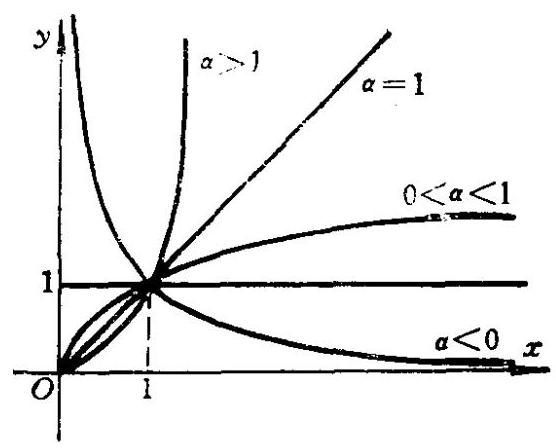
\includegraphics[max width=0.4\textwidth]{images/bo_d25ksc77aajc738obdgg_255_571_236_556_448_0.jpg}
\end{center}
\hspace*{3em} 

图 5-14

\section*{6)双曲函数}

定义 函数
\begin{align*}
	&x \mapsto  \operatorname{sh}x \triangleq  \frac{{e}^{x} - {e}^{-x}}{2},x \in  \mathbf{R};\\
	&x \mapsto  \operatorname{ch}x\;\frac{{e}^{x} + {e}^{-x}}{2},x \in  \mathbf{R};\\
	&x \mapsto  \operatorname{th}x \triangleq  \frac{{e}^{x} - {e}^{-x}}{{e}^{x} + {e}^{-x}},x \in  \mathbf{R};\\
	&x \mapsto  \operatorname{cth}x \triangleq  \frac{{e}^{x} + {e}^{-x}}{{e}^{x} - {e}^{-x}},x \in  \mathbf{R} - \{ 0\}
\end{align*}

分别称为双曲正弦函数、双曲余弦函数、双曲正切函数与双曲余切函数.

这些函数的基本性质可由下面两个定理来表述.

定理 $5 \cdot  4 \cdot  6\;1$ )双曲正弦、双曲余弦、双曲正 切、双曲余切函数都是在各自定义域上的连续函数.

2)下述等式成立:
\begin{align*}
	&{\operatorname{ch}}^{2}x - {\operatorname{sh}}^{2}x = 1,1 - {\operatorname{th}}^{2}x = \frac{1}{{\operatorname{ch}}^{2}x},\\
	&{\operatorname{cth}}^{2}x - 1 = \frac{1}{{\operatorname{sh}}^{2}x},\\
	&\operatorname{sh}\left( {-x}\right)  =  - \operatorname{sh}x,\operatorname{ch}\left( {-x}\right)  = \operatorname{ch}x,\\
	&\operatorname{th}\left( {-x}\right)  =  - \operatorname{th}x,\operatorname{cth}\left( {-x}\right)  =  - \operatorname{cth}x,\\
	&\operatorname{sh}\left( {x + y}\right)  = \operatorname{sh}x\operatorname{ch}y + \operatorname{ch}x\operatorname{sh}y,\\
	&\operatorname{ch}\left( {x + y}\right)  = \operatorname{ch}x\operatorname{ch}y + \operatorname{sh}x\operatorname{sh}y.
\end{align*}

证明 性质 1 )直接由双曲函数的定义推出 2 )的各等式直接计算即可验证.

定理 $5 \cdot  4 \cdot  7$ 关于双曲函数的单调性及其图形,我们有下述各结论:

1)双曲正弦函数在 $\mathbf{R}$ 上严格单调上升,并且
$$\mathop{\operatorname{lims}}\limits_{{x \rightarrow   - \infty }}\mathrm{h}x =  - \infty ,\mathop{\operatorname{limsh}}\limits_{{x \rightarrow   + \infty }}x =  + \infty .$$

它的图形关于原点对称, 无渐近线.

2) 双曲余弦函数在 $\lbrack 0, + \infty \lbrack$ 上严格单调上升,而在 $\rbrack  - \infty$ , 0 ]上是严格单调下降的, 并且
$$\mathop{\lim }\limits_{{x \rightarrow  0}}\operatorname{ch}x = 1,\mathop{\lim }\limits_{{x \rightarrow   \pm  \infty }}\operatorname{ch}x =  + \infty .$$

它的图形关于 $y$ 轴对称,无渐近线.

3) 双曲正切函数在 $\mathbf{R}$ 上严格单调上升,并且
$$\mathop{\lim }\limits_{{x \rightarrow   - \infty }}\operatorname{th}x =  - 1,\mathop{\lim }\limits_{{x \rightarrow   + \infty }}\operatorname{th}x = 1$$

它的图形关于原点对称,并且有无穷远分支 ${\Gamma }_{+\infty }$ 与 ${\Gamma }_{-\infty },{\Gamma }_{+\infty }$ 以 $y = 1$ 为水平渐近线, ${\Gamma }_{-\infty }$ 以 $y =  - 1$ 为水平渐近线.

4) 双曲余切函数在 $\mathbf{R} - \{ 0\}$ 上严格单调下降,并且
\begin{align*}
	&\mathop{\operatorname{limcth}}\limits_{{x \rightarrow   - \infty }}x =  - 1,\mathop{\operatorname{limcth}}\limits_{{x \rightarrow  0}}x =  - \infty ,\\
	&\mathop{\operatorname{limcth}}\limits_{{x \rightarrow  {0}^{ + }}}x =  + \infty ,\mathop{\operatorname{limcth}}\limits_{{x \rightarrow   + \infty }}x = 1.
\end{align*}

它的图形关于原点对称,并且有四个无穷远分支 ${\Gamma }_{-\infty },{\Gamma }_{0} -$ , ${\Gamma }_{{0}^{ + }},{\Gamma }_{+\infty }$ . ${\Gamma }_{-\infty }$ 以 $y =  - 1$ 为水平渐近线, ${\Gamma }_{0}$ -以负 $y$ 轴为垂直渐近线, ${\Gamma }_{0} +$ 以正 $y$ 轴为垂直渐近线,而 ${\Gamma }_{+\infty }$ 以 $y = 1$ 为水平渐近线.

证明 1) 设 ${x}_{1},{x}_{2} \in  \mathbf{R} - \{ 0\}$ ,并且 ${x}_{1} < {x}_{2}$ .

由以 $e$ 为底的指数函数的严格单调上升性, ${e}^{2{x}_{1}} < {e}^{2{x}_{2}}$ ,从而 $1 - {e}^{-2{x}_{2}} > 1 - {e}^{-2{x}_{1}}$ ,于是
\begin{align*}
	&\frac{\operatorname{sh}{x}_{2}}{\operatorname{sh}{x}_{1}} = \frac{{e}^{{x}_{2}} - {e}^{-{x}_{2}}}{{e}^{{x}_{1}} - {e}^{-{x}_{1}}}\\
	&= {e}^{{x}_{2} - {x}_{1}}\left( \frac{1 - {e}^{-2{x}_{2}}}{1 - {e}^{-2{x}_{1}}}\right)  > 1.
\end{align*}

此即表明双曲正弦函数在 $\mathbf{R} - \{ 0\}$ 上严格单调上升.

现设 ${x}_{1},{x}_{2} \in  \mathbf{R}$ ,并且 ${x}_{1} < 0 < {x}_{2}$ . 由定义知
$$\operatorname{sh}{x}_{1} < \operatorname{sh}0 = 0 < \operatorname{sh}{x}_{2}.$$

因此双曲正弦函数在 $R$ 上是严格单调上升的. 直接计算得到
$$\mathop{\operatorname{limsh}}\limits_{{x \rightarrow   - \infty }}x =  - \infty ,\mathop{\operatorname{limsh}}\limits_{{x \rightarrow   + \infty }}x =  + \infty .$$

由此可知双曲正弦函数的图形无渐近线,并且由 $\operatorname{sh}\left( {-x}\right)$  $=  - \operatorname{sh}x,\forall x \in  \mathbf{R}$ 知,此函数图形关于原点对称.

2) 因为 ${\mathrm{{ch}}}^{2}x - {\mathrm{{sh}}}^{2}x = 1\left( {\forall x \in  \mathbf{R}}\right)$ ,并且 $\mathrm{{ch}}x > 0$ ,所以 $\mathrm{{ch}}x$  $= \sqrt{1 + {\operatorname{sh}}^{2}x}\left( {\forall x \in  \mathbf{R}}\right)$ ,由此,并根据双曲正弦函数的严格单调上升性和 $\operatorname{sh}x < 0\left( {\forall x \in  {\mathbf{R}}_{ * }^{ - }}\right)$ 及 $\operatorname{sh}x > 0\left( {\forall x \in  {\mathbf{R}}_{ * }^{ + }}\right)$ 推知,双曲余弦函数 $\mathrm{{ch}}$ 在 $\left\lbrack  {0, + \infty \left\lbrack  \text{ 上严格单调上升,而在 }\right\rbrack   - \infty ,0}\right\rbrack$ 上严格单调下降.

现在直接由 $\operatorname{ch}x$ 的表达式计算得到
$$\mathop{\lim }\limits_{{x \rightarrow  0}}\operatorname{ch}x = 1,\mathop{\lim }\limits_{{x \rightarrow   \pm  \infty }}\operatorname{ch}x =  + \infty .$$

由此可知 $\mathrm{{ch}}$ 的图形无渐近线,并且由 $\mathrm{{ch}}\left( {-x}\right)  = \mathrm{{ch}}x$  $\left( {\forall x \in  \mathbf{R}}\right)$ 推知,双曲余弦函数 $\mathrm{{ch}}$ 的图形关于 $y$ 轴对称.

3) 由公式 ${\operatorname{th}}^{2}x = 1 - \frac{1}{{\operatorname{ch}}^{2}x}$ 及双曲余弦的单调性推知,双曲正切 $\mathrm{{th}}$ 在 $\mathbf{R}$ 上是严格单调上升的.

直接由 $\operatorname{th}x$ 的表达式计算得到
$$\mathop{\lim }\limits_{{x \rightarrow   - \infty }}\operatorname{th}x =  - 1,\mathop{\lim }\limits_{{x \rightarrow   + \infty }}\operatorname{th}x = 1.$$

由此可知双曲正切 $\operatorname{th}$ 图形有无穷远分支 ${\Gamma }_{-\infty }$ 与 ${\Gamma }_{+\infty }$ ,并且 ${\Gamma }_{-\infty }$ 以 $y$  $=  - 1$ 为水平渐近线, $\Gamma .\infty$ 以 $y = 1$ 为水平渐近线.

由于 $\operatorname{th}\left( {-x}\right)  =  - \operatorname{th}x,\forall x \in  \mathbf{R}$ ,故此函数图形关于原点对称

4) 由公式 ${\operatorname{cth}}^{2}x = 1 + \frac{1}{{\operatorname{sh}}^{2}x}$ 及双曲正弦的严格单调上升性推知,双曲余切函数在 $\mathbf{R} - \{ 0\}$ 上是严格单调下降的.

直接由 $\mathrm{c}\operatorname{lh}x$ 的表达式计算得到
\begin{align*}
	&\mathop{\lim }\limits_{{x \rightarrow   - \infty }}\operatorname{ch}x =  - 1,\mathop{\lim }\limits_{{x \rightarrow  {0}^{ - }}}\operatorname{cth}x =  - \infty ,\\
	&\mathop{\operatorname{limcth}}\limits_{{x \rightarrow  {0}^{ + }}}x =  + \infty ,\mathop{\operatorname{limcth}}\limits_{{x \rightarrow   + \infty }}x = 1.
\end{align*}

由此可知,双曲余切函数的图形有四个无穷远分支 ${\Gamma }_{-\infty },{\Gamma }_{0} -$ , ${\Gamma }_{0} \cdot$ 及 ${\Gamma }_{+\infty }$ ,并且 ${\Gamma }_{-\infty }$ 以 $y =  - 1$ 为水平渐近线, ${\Gamma }_{0} -$ 以负 $y$ 轴为垂直渐近线, ${\Gamma }_{{0}^{ + }}$ 以正 $y$ 轴为垂直渐近线,而 ${\Gamma }_{+\infty }$ 以 $y = 1$ 为水平渐近线.

最后由于 $\operatorname{cth}\left( {-x}\right)  =  - \operatorname{cth}x$ ,故此函数图形关于原点对称.

\begin{center}
	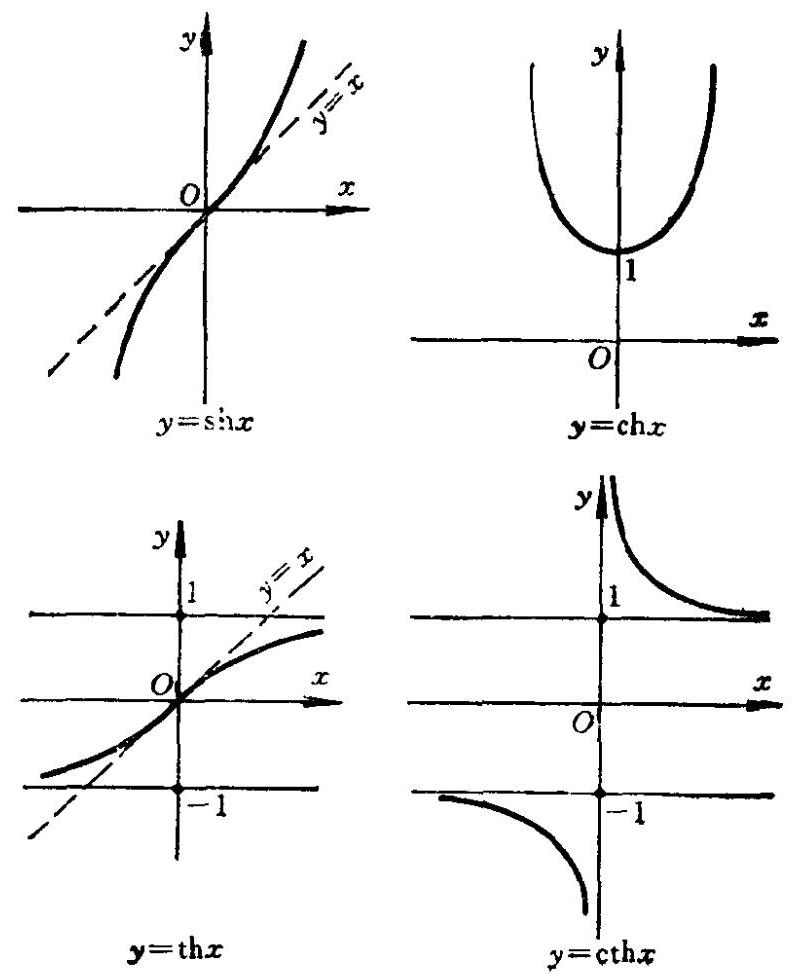
\includegraphics[max width=0.7\textwidth]{images/bo_d25ksc77aajc738obdgg_258_314_1120_795_974_0.jpg}
\end{center}
\hspace*{3em} 

图 5-15

图 5-15 是各双曲函数的大致图形.

\section*{7 )反双曲函数}

由定理 $5 \cdot  4 \cdot  7$ 知,双曲正弦、余弦、正切、余切分别是从 $\mathrm{R}$ 到 $\mathbf{R}$ 、从 $\lbrack 0, + \infty \lbrack$ 到 $\lbrack 1, + \infty \lbrack$ 、从 $\mathbf{R}$ 到 $\rbrack  - 1,1\lbrack$ 、从 $\mathbf{R} - \{ 0\}$ 到 $\mathbf{R} - \left\lbrack  {-1,1}\right\rbrack$ 上的严格单调的连续函数,根据定理 $4 \cdot  7 \cdot  1$ ,它们都有反函数存在.

定义 1 ) 函数 $\mathrm{{sh}} : \mathrm{R} \rightarrow  \mathrm{R}$ 的反函数称为反双曲正弦函数, 记为
$$\mathrm{{Arg}}\operatorname{sh} : \mathbf{R} \rightarrow  \mathbf{R}\text{ . }$$

2) 函数 ch: $\left\lbrack  {0, + \infty }\right\lbrack   \rightarrow  \lbrack 1, + \infty \lbrack$ 的反函数称为反双曲余弦函数, 记为
$$\text{ Arg ch: }\left\lbrack  {1, + \infty }\right\lbrack   \rightarrow  \lbrack 0, + \infty \lbrack \text{ . }$$

3) 函数 $\mathrm{{th}} : \mathrm{R} \rightarrow  \rbrack  - 1,1\lbrack$ 的反函数称为反双曲正切函数, 记为
$$\text{ Arg th:] } - 1,1\lbrack  \rightarrow  \mathbf{R}\text{ . }$$

4) 函数 eth: $\mathbf{R} - \{ 0\}  \rightarrow  \mathbf{R} - \left\lbrack  {-1,1}\right\rbrack$ 的反函数称为反双曲余切函数, 记为
$$\text{ Arg cth: }\mathbf{R} - \left\lbrack  {-1,1}\right\rbrack   \rightarrow  \mathbf{R} - \{ 0\} \text{ . }$$

定理 $5 \cdot  4 \cdot  8\;1$ ) 反双曲函数 Arg sh、Arg ch. Arg th、 Arg cth 除 Argcth 是严格单调下降外其余都是严格单调上升的连续函数.

2) 反双曲函数的显示表达式:

Arg $\operatorname{sh}x = \log \left( {x + \sqrt{{x}^{2} + 1}}\right) ,x \in  \mathbf{R}$ ;
\begin{align*}
	&\text{ Arg }\operatorname{ch}x = \log \left( {x + \sqrt{{x}^{2} - 1}}\right) ,x \in  \lbrack 1, + \infty \lbrack\\
	&\text{ Arg }\operatorname{th}x = \frac{1}{2}\log \frac{1 + x}{1 - x},x \in  \rbrack  - 1,1\lbrack \text{ ; }\\
	&\operatorname{Arg}\operatorname{cth}x = \frac{1}{2}\log \frac{x + 1}{x - 1},x \in  \mathbf{R} - \left\lbrack  {-1,1}\right\rbrack  .
\end{align*}

证明 性质 1 )显然, 下面我们来证明反双曲函数的显示表达式.

对 $\operatorname{Arg}\operatorname{sh}x$ : 由 $y = \operatorname{Arg}\operatorname{sh}x$ 得到 $x = \operatorname{sh}y$ . 因为
$$\operatorname{ch}y = \sqrt{{\operatorname{sh}}^{2}y + 1} = \sqrt{{x}^{2} + 1},$$

所以
$${e}^{y} = \operatorname{sh}y + \operatorname{ch}y = x + \sqrt{{x}^{2} + 1},$$

从而
$$\operatorname{Arg}\operatorname{sh}x = y = \log \left( {x + \sqrt{{x}^{2} + 1}}\right) .$$

对 $\operatorname{Arg}\operatorname{ch}x$ : 由 $y = \operatorname{Arg}\operatorname{ch}x$ 得到 $x = {\operatorname{ch}}^{y}$ . 于是
$$\operatorname{sh}y = \sqrt{{\operatorname{ch}}^{2}y - 1} = \sqrt{{x}^{2} - 1},$$

从而
$${e}^{y} = \operatorname{ch}y + \operatorname{sh}y = x + \sqrt{{x}^{2} - 1},$$

因此
$$\text{ Arg }\operatorname{ch}x = y = \log \left( {x + \sqrt{{x}^{2} - 1}}\right) \text{ . }$$

对 $\operatorname{Arg}\operatorname{th}x$ : 由 $y = \operatorname{Arg}\operatorname{th}x$ 得到 $x = \operatorname{th}y$ . 因为
$$\operatorname{th}y = \frac{{e}^{y} - {e}^{-y}}{{e}^{y} + {e}^{-y}} = \frac{{e}^{2y} - 1}{{e}^{2y} + 1},$$

所以 ${e}^{2y} = \frac{1 + x}{1 - x}$ ,从而
$$\text{ Arg th }x = y = \frac{1}{2}\log \frac{1 + x}{1 - x}\text{ . }$$

对 $\operatorname{Arg}\operatorname{cth}x$ : 由 $y = \operatorname{Arg}\operatorname{cth}x$ 得到 $x = {\operatorname{cth}}^{y}$ . 因为 ${\operatorname{cth}}^{y} =$  $\frac{{e}^{y} + {e}^{-y}}{{e}^{y} - {e}^{-y}} = \frac{{e}^{2y} + 1}{{e}^{2y} - 1}$

所以 ${e}^{2y} = \frac{x + 1}{x - 1}$ ,因此
$$\text{ Arg cth }x = y = \frac{1}{2}\log \frac{x + 1}{x - 1}\text{ . }$$

附注 反双曲函数 Arg sh、Arg ch、Arg th、Arg cth的图形可由相应双曲函数 sh、ch、th、cth 的图形关于直线 $y = x$ 的对称图形得到,有一点要注意,在作双曲余弦函数 $\mathrm{{ch}}$ 的图形关于 $y = x$ 的对称图形时,只有位于 $y \geq  0$ 上半平面的那一分支才是反双曲余弦Argch的图形.

\begin{center}
	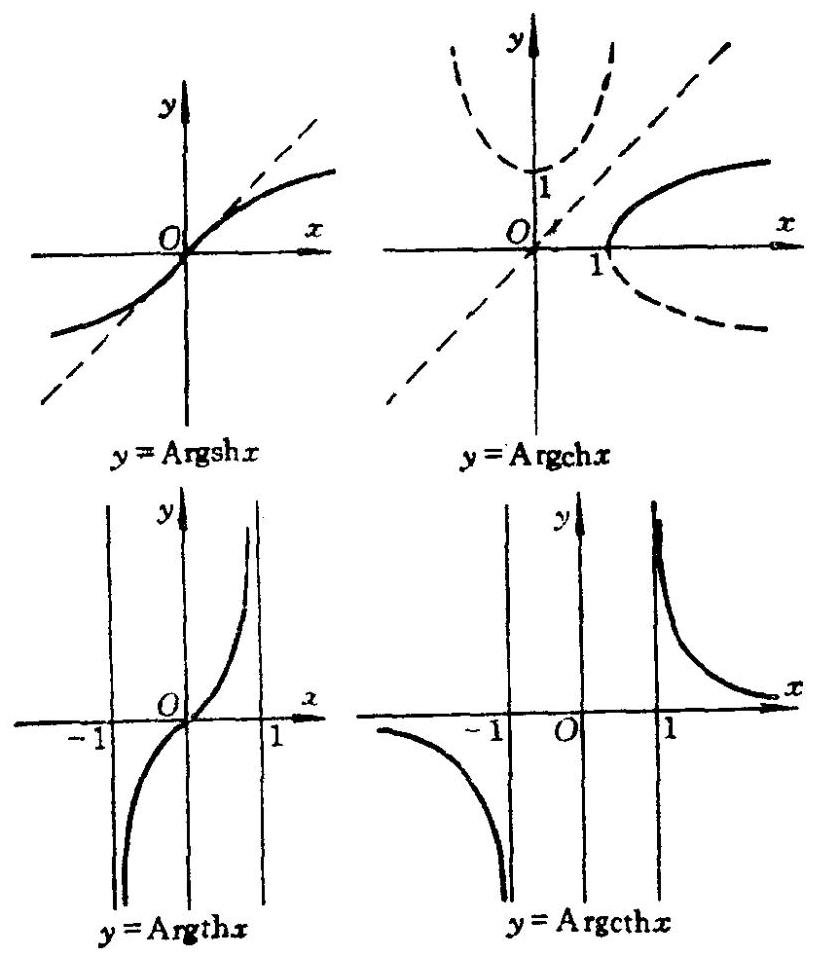
\includegraphics[max width=0.7\textwidth]{images/bo_d25ksc77aajc738obdgg_261_402_467_815_957_0.jpg}
\end{center}
\hspace*{3em} 

图 5-16

上面我们定义的七类函数连同有理整函数 (多项式函数). 有理分式函数、三角函数、反三角函数一起统称为基本初等函数.

由基本初等函数经过有限次加、减、乘、除四则运算及函数的复合所得到的函数称为有限形式的初等函数.

作为初等函数的一个例子, 我们介绍所谓的幂指数函数.

幂指数函数 设 $u,v : X \rightarrow  \mathrm{R}$ 是任意两个函数,使得 $\forall x \in$  $X,u{\left( x\right) }^{v\left( x\right) }$ 有定义,则函数
$$x \mapsto  u{\left( x\right) }^{v\left( x\right) },x \in  X$$

你为幂指数函数. 我们设 $a \in  X$ 是一聚点.

1) 若 $\mathop{\lim }\limits_{{x \rightarrow  a}}u\left( x\right)  = A > 0,\mathop{\lim }\limits_{{x \rightarrow  a}}v\left( x\right)  = B$ ,则
\begin{align*}
	&\mathop{\lim }\limits_{{x \rightarrow  a}}u{\left( x\right) }^{v\left( x\right) } = \mathop{\lim }\limits_{{x \rightarrow  a}}{e}^{v\left( x\right) \log u\left( x\right) }\\
	&= {e}^{\mathop{\lim }\limits_{{x \rightarrow  a}}v\left( x\right) \log u\left( x\right) }\\
	&= {e}^{B\log A}\\
	&= {A}^{B}\text{ . }
\end{align*}

2) 若 $\mathop{\lim }\limits_{{x \rightarrow  a}}u\left( x\right)  = 0$ ,但 $\mathop{\lim }\limits_{{x \rightarrow  a}}v\left( x\right) \log u\left( x\right)  = c$ ,则
\begin{align*}
	&\mathop{\lim }\limits_{{x \rightarrow  a}}u{\left( x\right) }^{v\left( x\right) } = \mathop{\lim }\limits_{{x \rightarrow  a}}{e}^{v\left( x\right) \log u\left( x\right) }\\
	&= {e}^{\mathop{\lim }\limits_{{x \rightarrow  a}}v\left( x\right) \log u\left( x\right) }\\
	&= \left\{  \begin{array}{ll} {e}^{c}, & \text{ 若 }c \in  \mathbf{R}, \\   + \infty , & \text{ 若 }c =  + \infty , \\  0, & \text{ 若 }c =  - \infty . \end{array}\right.
\end{align*}

3) 若 $\mathop{\lim }\limits_{{x \rightarrow  a}}u\left( x\right)  = A,\mathop{\lim }\limits_{{x \rightarrow  a}}v\left( x\right)  = B$ 出现下列三种情形:
$$A = 1,B =  \pm  \infty ;A = 0,B = 0;A =  \pm  \infty ,B = 0.$$

则 $u{\left( x\right) }^{v\left( x\right) }$ 分别为 ${1}^{\pm \infty },{0}^{0}, \pm  {\infty }^{0}$ 不定型,这种不定型极限的一般研究我们将在以后进行.

下面介绍一个典型的 ${1}^{\infty }$ 不定型极限.

例1 证明

1) $\mathop{\lim }\limits_{{x \rightarrow  0}}{\left( 1 + x\right) }^{\frac{1}{x}} = e$ .

2) $\mathop{\lim }\limits_{{x \rightarrow   \pm  \infty }}{\left( 1 + \frac{1}{x}\right) }^{x} = e$ ,
$$\mathop{\lim }\limits_{{n \rightarrow   \pm  \infty }}{\left( 1 + \frac{1}{n}\right) }^{n} = e,\left( {n \in  \mathbf{Z}}\right) .$$

3) $\mathop{\lim }\limits_{{h \rightarrow  0}}{\left( 1 + hx\right) }^{\frac{1}{h}} = {e}^{x},\forall x \in  \mathbf{R}$ .

首先我们考虑 $\mathop{\lim }\limits_{{x \rightarrow  0}}{\left( 1 + x\right) }^{\frac{1}{x}}$ . 这是 ${1}^{ \sim  }$ 不定型极限. 当 $\left| x\right|$ 充分小时, $1 + x > 0$ ,因此
$${\left( 1 + x\right) }^{\frac{1}{x}} = {e}^{\frac{1}{x}\log \left( {1 + x}\right) }.$$

由于 $\log \left( {1 + x}\right)  = {\int }_{1}^{1 + x}\frac{1}{t}{dt}$ ,故由第一积分中值公式知,
$$\log \left( {1 + x}\right)  = \frac{1}{\xi }{\int }_{1}^{1 + x}{dt} = \frac{x}{\xi }.$$

这里 $\xi$ 介于 1 与 $1 + x$ 之间,从而 $\xi  \rightarrow  1\left( {x \rightarrow  0}\right)$ . 因此
\begin{align*}
	&\mathop{\lim }\limits_{{x \rightarrow  0}}{\left( 1 + x\right) }^{\frac{1}{x}} = \mathop{\lim }\limits_{{x \rightarrow  0}}{e}^{\frac{1}{x}\log \left( {1 + x}\right) }\\
	&= {e}^{\mathop{\lim }\limits_{{x \rightarrow  0}}\frac{1}{x}\log \left( {1 + x}\right) }\\
	&= {e}^{\dot{x}\overset{1 \cdot  m}{ \rightarrow  }\dot{\xi }}\\
	&= e\text{ . }
\end{align*}

现在我们令 $y = \frac{1}{x}$ ,则 $y \rightarrow  0\left( {x \rightarrow   \pm  \infty }\right)$ . 从而
$$\mathop{\lim }\limits_{{x \rightarrow   \pm  \infty }}{\left( 1 + \frac{1}{x}\right) }^{x} = \mathop{\lim }\limits_{{y \rightarrow  0}}{\left( 1 + y\right) }^{\frac{1}{y}} = e.$$

特别地取 $x = n \in  \mathbf{Z}$ ,则
$$\mathop{\lim }\limits_{{n \rightarrow   \pm  \infty }}{\left( 1 - \frac{1}{n}\right) }^{n} = e$$

最后令 $y = {hx}$ ,当 $x = 0$ 时 $y = 0$ ,并且 $y \rightarrow  0\left( {h \rightarrow  0}\right)$ . 因此
\begin{align*}
	&\mathop{\lim }\limits_{{h \rightarrow  0}}{\left( 1 + hx\right) }^{\frac{1}{h}} = \mathop{\lim }\limits_{{y \rightarrow  0}}{\left\lbrack  {\left( 1 + y\right) }^{\frac{1}{y}}\right\rbrack  }^{x}\\
	&= {\left\lbrack  \mathop{\lim }\limits_{{y \rightarrow  0}}{\left( 1 + y\right) }^{\frac{1}{y}}\right\rbrack  }^{x}\\
	&= {e}^{x}\text{ . }
\end{align*}

当 $x = 0$ 时, $\mathop{\lim }\limits_{{h \rightarrow  0}}{\left( 1 + hx\right) }^{\frac{1}{h}} = 1 = {e}^{0}$ .

例 2 证明: $\forall \alpha  \in  \mathbf{R},\mathop{\lim }\limits_{{x \rightarrow  0}}\frac{{\left( 1 + x\right) }^{\alpha } - 1}{x} = \alpha$ .

为此令 ${\left( 1 + x\right) }^{a} - 1 = y$ ,则 $y \rightarrow  0\left( {x \rightarrow  0}\right)$ ,并且 ${\left( 1 + x\right) }^{a} = 1 +$  $y$ . 于是 $\alpha \log \left( {1 + x}\right)  = \log \left( {1 + y}\right)$ ,从而
\begin{align*}
	&\mathop{\lim }\limits_{{x \rightarrow  0}}\frac{{\left( 1 + x\right) }^{a} - 1}{x} = \mathop{\lim }\limits_{{x \rightarrow  0}}\frac{y}{x}\\
	&= \mathop{\lim }\limits_{{x \rightarrow  0}}\frac{y}{\log \left( {1 + y}\right) } \cdot  \frac{\alpha \log \left( {1 + x}\right) }{x}\\
	&= \mathop{\lim }\limits_{{y \rightarrow  \infty }}\frac{1}{\log {\left( 1 + y\right) }^{\frac{1}{y}}} \cdot  \mathop{\lim }\limits_{{x \rightarrow  0}}\alpha \log {\left( 1 + x\right) }^{\frac{1}{x}}\\
	&= \alpha  \cdot  \frac{1}{\log e} \cdot  \log e\\
	&= a\text{ . }
\end{align*}

例 3 计算 $\mathop{\lim }\limits_{{x \rightarrow  0}}{\left( \frac{1 + \operatorname{tg}x}{1 + \sin x}\right) }^{\frac{1}{\sin x}}$ .

这是 ${1}^{\infty }$ 不定型极限,我们把它化为 $\mathop{\lim }\limits_{{x \rightarrow  0}}{\left( 1 + x\right) }^{\frac{1}{x}}$ 型极限进行计算.
\begin{align*}
	&\mathop{\lim }\limits_{{x \rightarrow  0}}{\left( \frac{1 + \operatorname{tg}x}{1 + \sin x}\right) }^{\frac{1}{\sin x}}\\
	&= \mathop{\lim }\limits_{{x \rightarrow  0}}{\left( 1 + \frac{\operatorname{tg}x - \sin x}{1 + \sin x}\right) }^{\frac{1}{\frac{\operatorname{tg}x - \sin x}{1 + \sin x}} \cdot  \frac{\operatorname{tg}x - \sin x}{1 + \sin x} \cdot  \frac{1}{\sin x}}\\
	&= {\left\lbrack  \mathop{\lim }\limits_{{y \rightarrow  0}}{\left( 1 + y\right) }^{\frac{1}{y}}\right\rbrack  }^{\frac{\mathop{\lim }\limits_{{x \rightarrow  0}}\frac{1}{\cos x} - \cos x}{\cos x\left( {1 + \sin x}\right) }}\\
	&= {e}^{0}\\
	&= 1\text{ . }
\end{align*}

最后作为这一节的结束, 我们来考虑下面的一个重要极限, 在第 6 章 $§2$ 中我们将要用到它.

例 4 证明: $\forall \alpha  > 0,\mathop{\lim }\limits_{{x \rightarrow   + \infty }}\frac{{e}^{x}}{{x}^{\alpha }} =  + \infty$ .

我们只需证明 $x = n \in  \mathbf{N}$ 时极限成立即可.

事实上,如果 $\mathop{\lim }\limits_{{n \rightarrow   + \infty }}\frac{{e}^{n}}{{n}^{a}} =  + \infty$ ,那末由函数 $x \mapsto  {e}^{x},x \in$  $\rbrack 0, + \infty \left\lbrack  {\text{ 及 }x \mapsto  {x}^{\alpha },x \in  \rbrack 0, + \infty \lbrack }\right.$ 的严格单调上升性我们有: $\forall x > 0$
$$\frac{{e}^{x}}{{x}^{a}} \geq  \frac{{e}^{\left\lbrack  x\right\rbrack  }}{{\left( \left\lbrack  x\right\rbrack   + 1\right) }^{a}} = \frac{1}{e}\frac{{e}^{\left\lbrack  x\right\rbrack   + 1}}{{\left( \left\lbrack  x\right\rbrack   + 1\right) }^{a}}.$$

由于 $\mathop{\lim }\limits_{{x \rightarrow   + \infty }}\left( {\left\lbrack  x\right\rbrack   + 1}\right)  =  + \infty$ ,故 $\mathop{\lim }\limits_{{x \rightarrow   + \infty }}\frac{{e}^{\left\lbrack  x\right\rbrack   + 1}}{{\left( \left\lbrack  x\right\rbrack   + 1\right) }^{a}} =  + \infty$ ,从而
$$\mathop{\lim }\limits_{{x \rightarrow   + \infty }}\frac{{e}^{x}}{{x}^{a}} =  + \infty$$

下面我们就来证明 $\mathop{\lim }\limits_{{n \rightarrow   + \infty }}\frac{{e}^{n}}{{n}^{a}} =  + \infty$ .

固定 $k \in  \mathbf{N}$ 使 $k > \alpha$ . 令 $h = e - 1,\forall n > k$ ,有
\begin{align*}
	&\frac{{e}^{n}}{{n}^{a}} = \frac{{\left( 1 + h\right) }^{n}}{{n}^{a}} > \frac{{C}_{n}^{k + 1}{h}^{k + 1}}{{n}^{k}}\\
	&= \frac{n\left( {n - 1}\right) \left( {n - 2}\right) \cdots \left( {n - k}\right) }{\left( {k + 1}\right) !{n}^{k}}{h}^{k + 1}\\
	&= n\left( {1 - \frac{1}{n}}\right) \left( {1 - \frac{2}{n}}\right) \cdots \left( {1 - \frac{k}{n}}\right) \frac{{h}^{k + 1}}{\left( {k + 1}\right) !}.
\end{align*}

由于 $\frac{{h}^{k + 1}}{\left( {k + 1}\right) !} > 0$ 为常数,
$$\mathop{\lim }\limits_{{n \rightarrow   + \infty }}\left( {1 - \frac{1}{n}}\right) \left( {1 - \frac{2}{n}}\right) \cdots \left( {1 - \frac{k}{n}}\right)  = 1,$$

14 $\mathop{\lim }\limits_{{n \rightarrow   + \infty }}n\left( {1 - \frac{1}{n}}\right) \left( {1 - \frac{2}{n}}\right) \cdots \left( {1 - \frac{k}{n}}\right) \frac{{h}^{k + 1}}{\left( {k + 1}\right) !} =  + \infty$ ,从而
$$\mathop{\lim }\limits_{{n \rightarrow   + \infty }}\frac{{e}^{n}}{{n}^{a}} =  + \infty$$

\section*{习 题}

1. 证明定理 $5 \cdot  4 \cdot  2\text{ 、 }5 \cdot  4 \cdot  4\text{ 、 }5 \cdot  4 \cdot  5\text{ 、 }5 \cdot  4 \cdot  6$ .

2. 设 $f : \left\lbrack  {a,b}\right\rbrack   \rightarrow  {R}^{ + }$ 是任一连续函数. 证明:

1) ${\left\lbrack  {\int }_{a}^{b}{f}^{n}\left( x\right) dx\right\rbrack  }^{-\frac{1}{n}} \leq  {\left( b - a\right) }^{-\frac{1}{n}}\mathop{\sup }\limits_{{a < x < b}}f\left( x\right) ,\forall n \in  \mathbf{N}$ .

2) 利用 $f$ 的连续性及确界特性证明:
\begin{align*}
	&\left( {\forall \varepsilon  > 0}\right) \left( {\exists \delta  > 0}\right)  \Rightarrow  {\left\lbrack  {\int }_{a}^{b}{f}^{n}\left( x\right) dx\right\rbrack  }^{\frac{1}{n}}\\
	&\geq  {\delta }^{\frac{1}{n}}\left( {\mathop{\sup }\limits_{{a \leq  x \leq  b}}f\left( x\right)  - \varepsilon }\right) .
\end{align*}

3) 由此推出 $\mathop{\lim }\limits_{{n \rightarrow   + \infty }}{\left\lbrack  {\int }_{a}^{b}{f}^{n}\left( x\right) dx\right\rbrack  }^{\frac{1}{n}} = \mathop{\sup }\limits_{{a \leq  x \leq  b}}f\left( x\right)$ .

4 ) 若 $g : \left\lbrack  {a,b}\right\rbrack   \rightarrow  {\mathrm{R}}^{ + }$ 是任一Riemann可积函数,则
$$\mathop{\lim }\limits_{{n \rightarrow   + \infty }}{\left\lbrack  {\int }_{a}^{b}{f}^{n}\left( x\right) g\left( x\right) dx\right\rbrack  }^{\frac{1}{n}} = \mathop{\sup }\limits_{{a \leq  x < b}}f\left( x\right) .$$

3. 设 ${x}_{n} = \sqrt[n]{\left\lbrack  {1 + {\left( \frac{1}{n}\right) }^{2}}\right\rbrack  \left\lbrack  {1 + {\left( \frac{2}{n}\right) }^{2}}\right\rbrack  \cdots \left\lbrack  {1 + {\left( \frac{n}{n}\right) }^{2}}\right\rbrack  }$ ,
$${y}_{n} = {\left( \sqrt[{n + 1}]{n} \cdot  \sqrt[{n + 2}]{2n} \cdot  \cdots  \cdot  \sqrt[{2n}]{{n}^{2}}\right) }^{\frac{1}{1 \cdot  0 \cdot  g \cdot  n}},$$

试研究序列 $\left\langle  {x}_{n}\right\rangle$ 与 $\left\langle  {y}_{n}\right\rangle$ 的收敛性,并求其极限.

4. 计算下列各极限:

1) $\mathop{\lim }\limits_{{x \rightarrow  0}}\frac{\log a\left( {1 + x}\right) }{x}\left( {0 < a = 1}\right)$ ,

2) $\mathop{\lim }\limits_{{x \rightarrow  0}}\frac{{a}^{x} - 1}{x}\left( {a > 0}\right)$ ,

3) $\mathop{\lim }\limits_{{x \rightarrow  0}}\frac{\sqrt[n]{1 + {ax}} - \sqrt[m]{1 + {bx}}}{x}$ ,

4) $\mathop{\lim }\limits_{{x \rightarrow  1}}{x}^{\frac{1}{1 - x}}$

5) $\lim {\left( \operatorname{tg}x\right) }^{\operatorname{tr}{2x}}$ ,

6) $\mathop{\lim }\limits_{{x \rightarrow  1}}{\left( 1 + \sin \pi x\right) }^{\operatorname{ctg}{\pi x}}$

7) $\mathop{\lim }\limits_{{x \rightarrow  0}}{\left( \frac{{a}_{1}{}^{x} + {a}_{2}{}^{t} + \cdots  + {a}_{n}{}^{t}}{n}\right) }^{\frac{1}{x}}\left( {{a}_{i} > 0}\right)$ ,

8) $\mathop{\lim }\limits_{{h \rightarrow  0}}\frac{\log \left( {x + h}\right)  + \log \left( {x - h}\right)  - 2\log x}{{h}^{2}}$ ,

9) $\mathop{\lim }\limits_{{x \rightarrow   + \infty }}{\left( \sin \frac{1}{x} + \cos \frac{1}{x}\right) }^{x}$ ,

10) $\mathop{\lim }\limits_{{x \rightarrow  0}} - \frac{\operatorname{sh}x}{x}$ ,

11) $\mathop{\lim }\limits_{{x \rightarrow  0}}\frac{\operatorname{ch}{2x} - 1}{{x}^{2}}$ ,

12) $\mathop{\lim }\limits_{{x \rightarrow  0}}\frac{{e}^{\ln {2x}} - {e}^{\ln x}}{\operatorname{th}x}$ ,

13) $\mathop{\lim }\limits_{{x \rightarrow  0}}\frac{{\operatorname{sh}}^{2}x}{\log \left( {\operatorname{ch}{2x}}\right) }$ ,

14) $\mathop{\lim }\limits_{{x \rightarrow   + \infty }}{\left( \frac{\operatorname{ch}\frac{\pi }{x}}{\cos \frac{\pi }{x}}\right) }^{{x}^{2}}$ .

